\documentclass[12pt,a4paper]{article}

%----- Packages ----
\usepackage{graphicx}       % For images
\usepackage{amsmath}        % Math symbols
\usepackage{lipsum}         % For dummy text
\usepackage{fancyhdr}       % For header/footer
\usepackage{geometry}       % Page margins
\usepackage{hyperref}       % Clickable links
\usepackage{setspace}       % Line spacing
\usepackage{float}
\usepackage{hyperref}

% Disable paragraph indentation
\setlength{\parindent}{0pt}

% Small space between paragraphs
\setlength{\parskip}{0.4em}  

%---- Page Setup -----
\geometry{margin=1in}
\onehalfspacing
\pagestyle{fancy}
\fancyhf{}
\rhead{Modeling Power Plant Energy Output}
\lhead{Rajesh Kumar Dhimal}
\cfoot{\thepage}

%----- Title Page -----
\begin{document}

\begin{titlepage}
    \centering
    %\vspace*{0.1cm}
    
    
\includegraphics[width=0.9\linewidth]{softwarica_covventry.png}

    \vspace{1cm}

    {\Huge \bfseries Modeling Power Plant Energy Output Using Nonlinear Regression \par}
    \vspace{1.5cm}
    
    %
\includegraphics[width=0.9\linewidth]{softwarica_covventry.png}

    {\Large \textbf{Assignment Report} \par}
    \vspace{1.5cm}
    
    \textbf{Submitted By:} \\
    {\large Rajesh Kumar Dhimal} \\
    Coventry University Student ID: 16542745 \\
    Softwarica Student ID: 250072 \\
    Faculty of Engineering, Environment and Computing  \\
    Coventry University, \\ 
    Softwarica College of IT and E-commerce
    \vspace{1cm}
    
    \textbf{Supervised By:} \\
    Lecturer Hikmat Saud \\
    7089 CEM: Introduction to Statistical Methods for Data Science \\
    \vspace{2cm}
    
    \vspace{1cm}
    {\large \today \par}
    \vfill

\end{titlepage}

%------Abstract------

\maketitle

\begin{abstract}

We were requested to figure out better performing model to predict net 
hourly electrical energy output of a Combined Cycle Power Plant (CCPP) from given
five non-linear regression models. We were requsted to use Ordinary
Least Squares Method to estimate optimum model parameters for the given models. The models were 
evaluated using various performance metrics like Residual Sum of Squares (RSS), 
log-likelihood (LL), Akaike Information Criterion (AIC), Bayesian Information Criterian (BIC); 
other regression metrics like Root Mean Squared Error(RMSE), R-squared ($R^2$) 
along with analysis of residual distribution.The selected model was then validated 
by 70-30 train-test split with 95\% confidence intervals.
 
Finally, Approximate Bayesian Computation (ABC) was used to 
estimate the posterior distributions of key parameters, allowing 
us to quantify uncertainty in predictions and better understand the system dynamics.

\end{abstract}

%-----------------------------------Introduction------------------------------

\section*{Introduction}

In Combined Cycle Power Plants (CCPPs), 
%use both gas and steam turbines to generate electricity are favourate among many because of their 
%high efficiency, low cost and low envoronmental impacts. In these systems, 
%the waste 
heat generated from the gas turbine is reused to generate electricity by powering the 
steam turbine. Doing so enhances the efficiency of the power houses and hence maximizes the output 
for the same investment.  

Our focus in this study was to predict the net energy output of a CCPP 
using given nonlinear regression models that capture relationships 
between the given variables and electrical energy output. %We evaluate given models 
%using metrics like RSS, AIC, BIC, MSE, r-squared, RMSE, MPE, Adjusted $R^2$ and apply Approximate Bayesian 
%Computation (ABC) to estimate uncertainty in key parameters, aiming for 
%accurate and actionable predictions.

%-----Data Description------

\section*{Dataset Description}

The data %was was collected from a real Combined Cycle 
%Power Plant (CCPP) operating continuously from 2006 to 2011. It 
consists 
of more than 9500 hourly observations, each capturing the plant's operating conditions. 
The data reflects varying environmental and operational conditions like the humidity in the air, vaccum 
level inside the machine, tempratue of the place, 
making it suitable for building predictiive models. 

The dataset has four input variables (environmental) and one output variable:

\begin{itemize}
  \item \textbf{x1 (T)}: Temperature: outside air temperature.
  \item \textbf{x3 (AP)}: Pressure: inside the gas turbine.
  \item \textbf{x4 (V)}: Exhaust Vacuum: pressure in the condenser of the steam turbine.
  \item \textbf{x5 (RH)}: Relative Humidity: the moisture content of air.
  \item \textbf{y (EP)}: Electricity output (hourly): our target variable.
\end{itemize}

%-------Preliminary Data Analysis------

\section*{Task 1: Preliminary Data Analysis}

\subsection*{Task 1.1: Data Preparation}
%The data was first loaded from a CSV file into the working 
%environment- R and Jupyter Notebooks. The dimensions of the dataset were checked to understand its 
%overall shape. No missing values were found in any of the columns. 
%However, a check for duplicated rows revealed 41 duplicate entries, 
%which were subsequently removed to ensure data quality. 

The data was uploaded into the system and primary works like data cleaning, data exploration, handeling
missing values and handeling duplicates were performed to make it suitable for modeling.  

To support further time series analysis, a new 'time' 
column was added, and columns were re-arranged so the output column \texttt{Energy Output (x2)} becomes 
the last column and \texttt{Time} becomes the first; a general convension in machine learning 
community.

%incrementing by one unit for 
%each record to represent hourly intervals. Finally, the columns 
%were reordered for better readability and structure in 
%the following order: \texttt{Time}, \texttt{Temperature (x1)}, 
%\texttt{Pressure (x3)}, \texttt{Humidity (x5)}, \texttt{Vacuum (x4)}, and 
%\texttt{Energy Output (x2)}. Final dataset contains 9527 rows and 6 columns, 
%including the dependent variable x2.

%-----Time Series Plots------
\subsection*{Task 1.2: Time Series Analysis}

%To get an initial overview of how the variables behave 
%over time, 
Time series plots were created for each variable by placing time series values
along x-axis and their corresponding readings along y-axis. 
Time series plots visually represent how the data varies and behaves across 
the entire collection period. %Analyzing them helps us to get understanding of overall spread 
%patterns, fluctuations and potential relationship between different variables.

\begin{figure}[H]
    \centering
    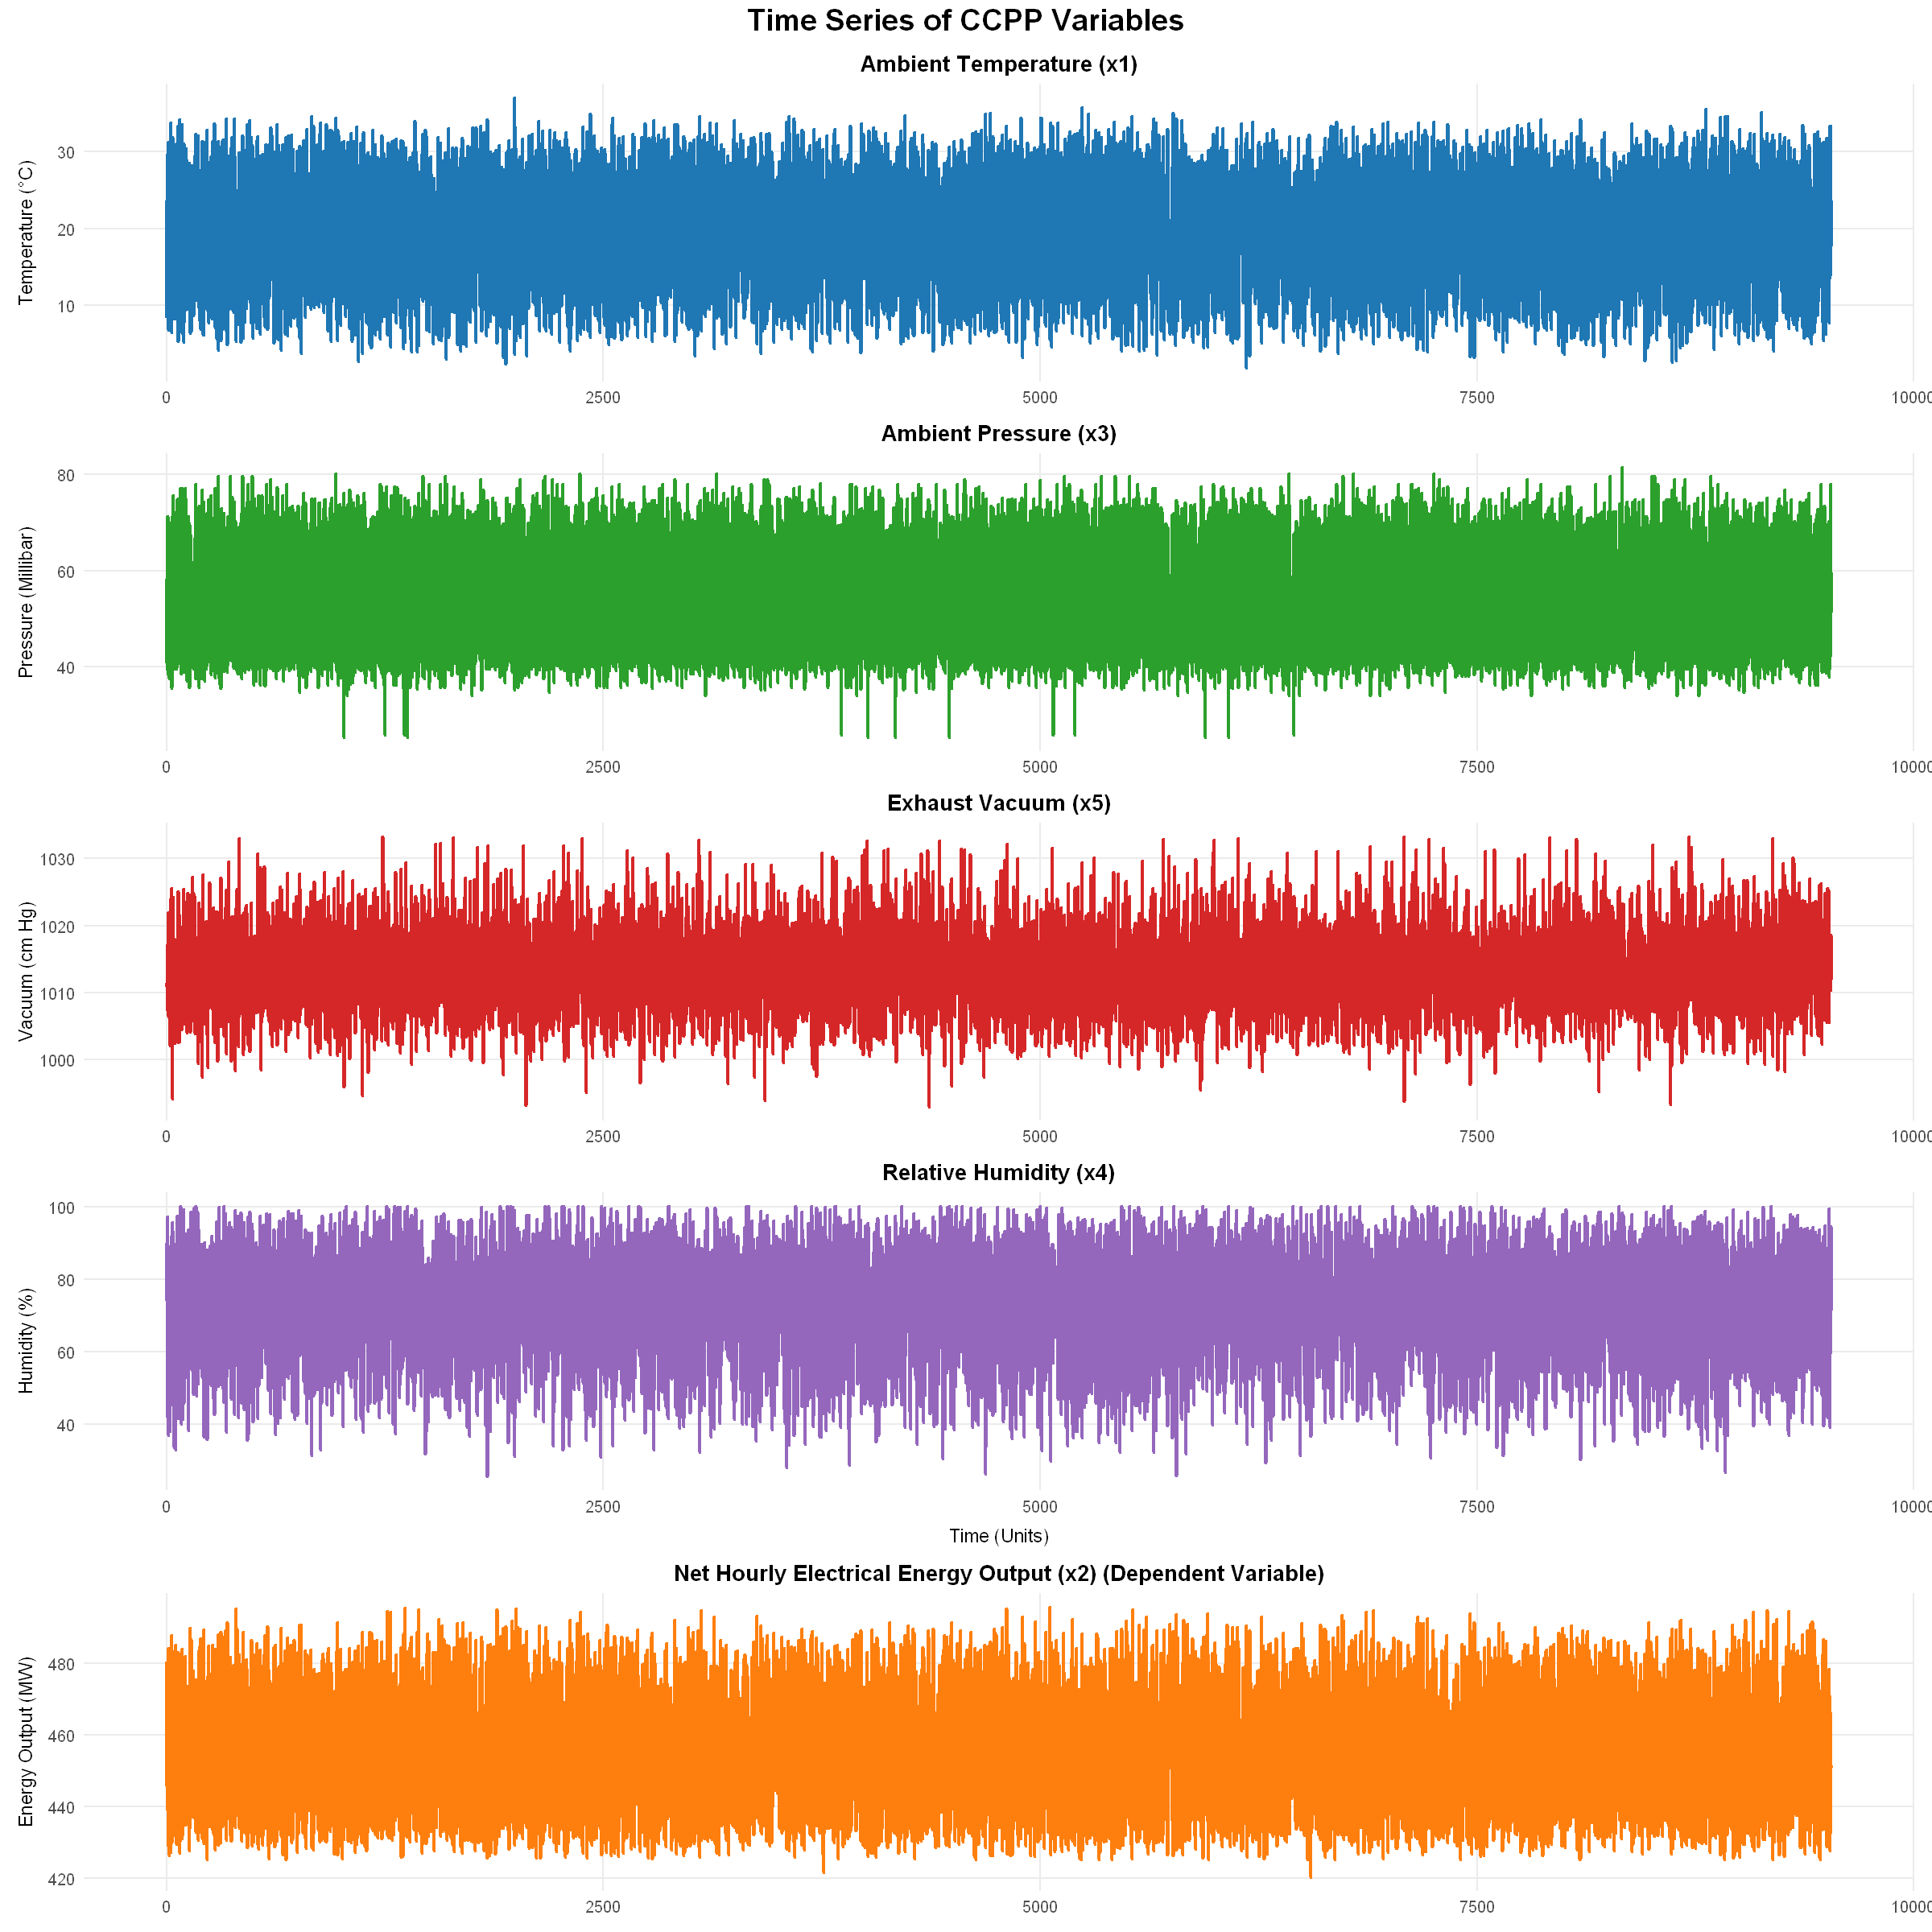
\includegraphics[width=\textwidth]{z3.png}
    \caption{(Time series plots of all five variables stacked 
    vertically: Ambient Temperature (\(x_1\)), Ambient Pressure  
    (\(x_3\)), Exhaust Vaccum (\(x_4\)), Relative Humidity (\(x_5\)), 
    and Net Hourly Electrical Energy Output (\(x_2\)) plotted against time (in hours))}
    \label{fig:time_series}
\end{figure}

%Fig shows five time series plots arranged vertically one after another.  
%The x-axis represents time in unit intervals, 
%while the y-axis shows the measured values for each variable. 

These plots illustrate how each variable fluctuates over the six-years 
period from 2006 to 2011. Due to the very high frequency in data, over 9,500 hourly records, 
all the plots appear very dense and noisy, 
making it difficult to spot meaningful trends. To address this, a rolling 
average with a window of 100 observations was applied to each variable. %This 
%smooths out visual noise and revealed clearer trends.

\begin{figure}[H]
    \centering
    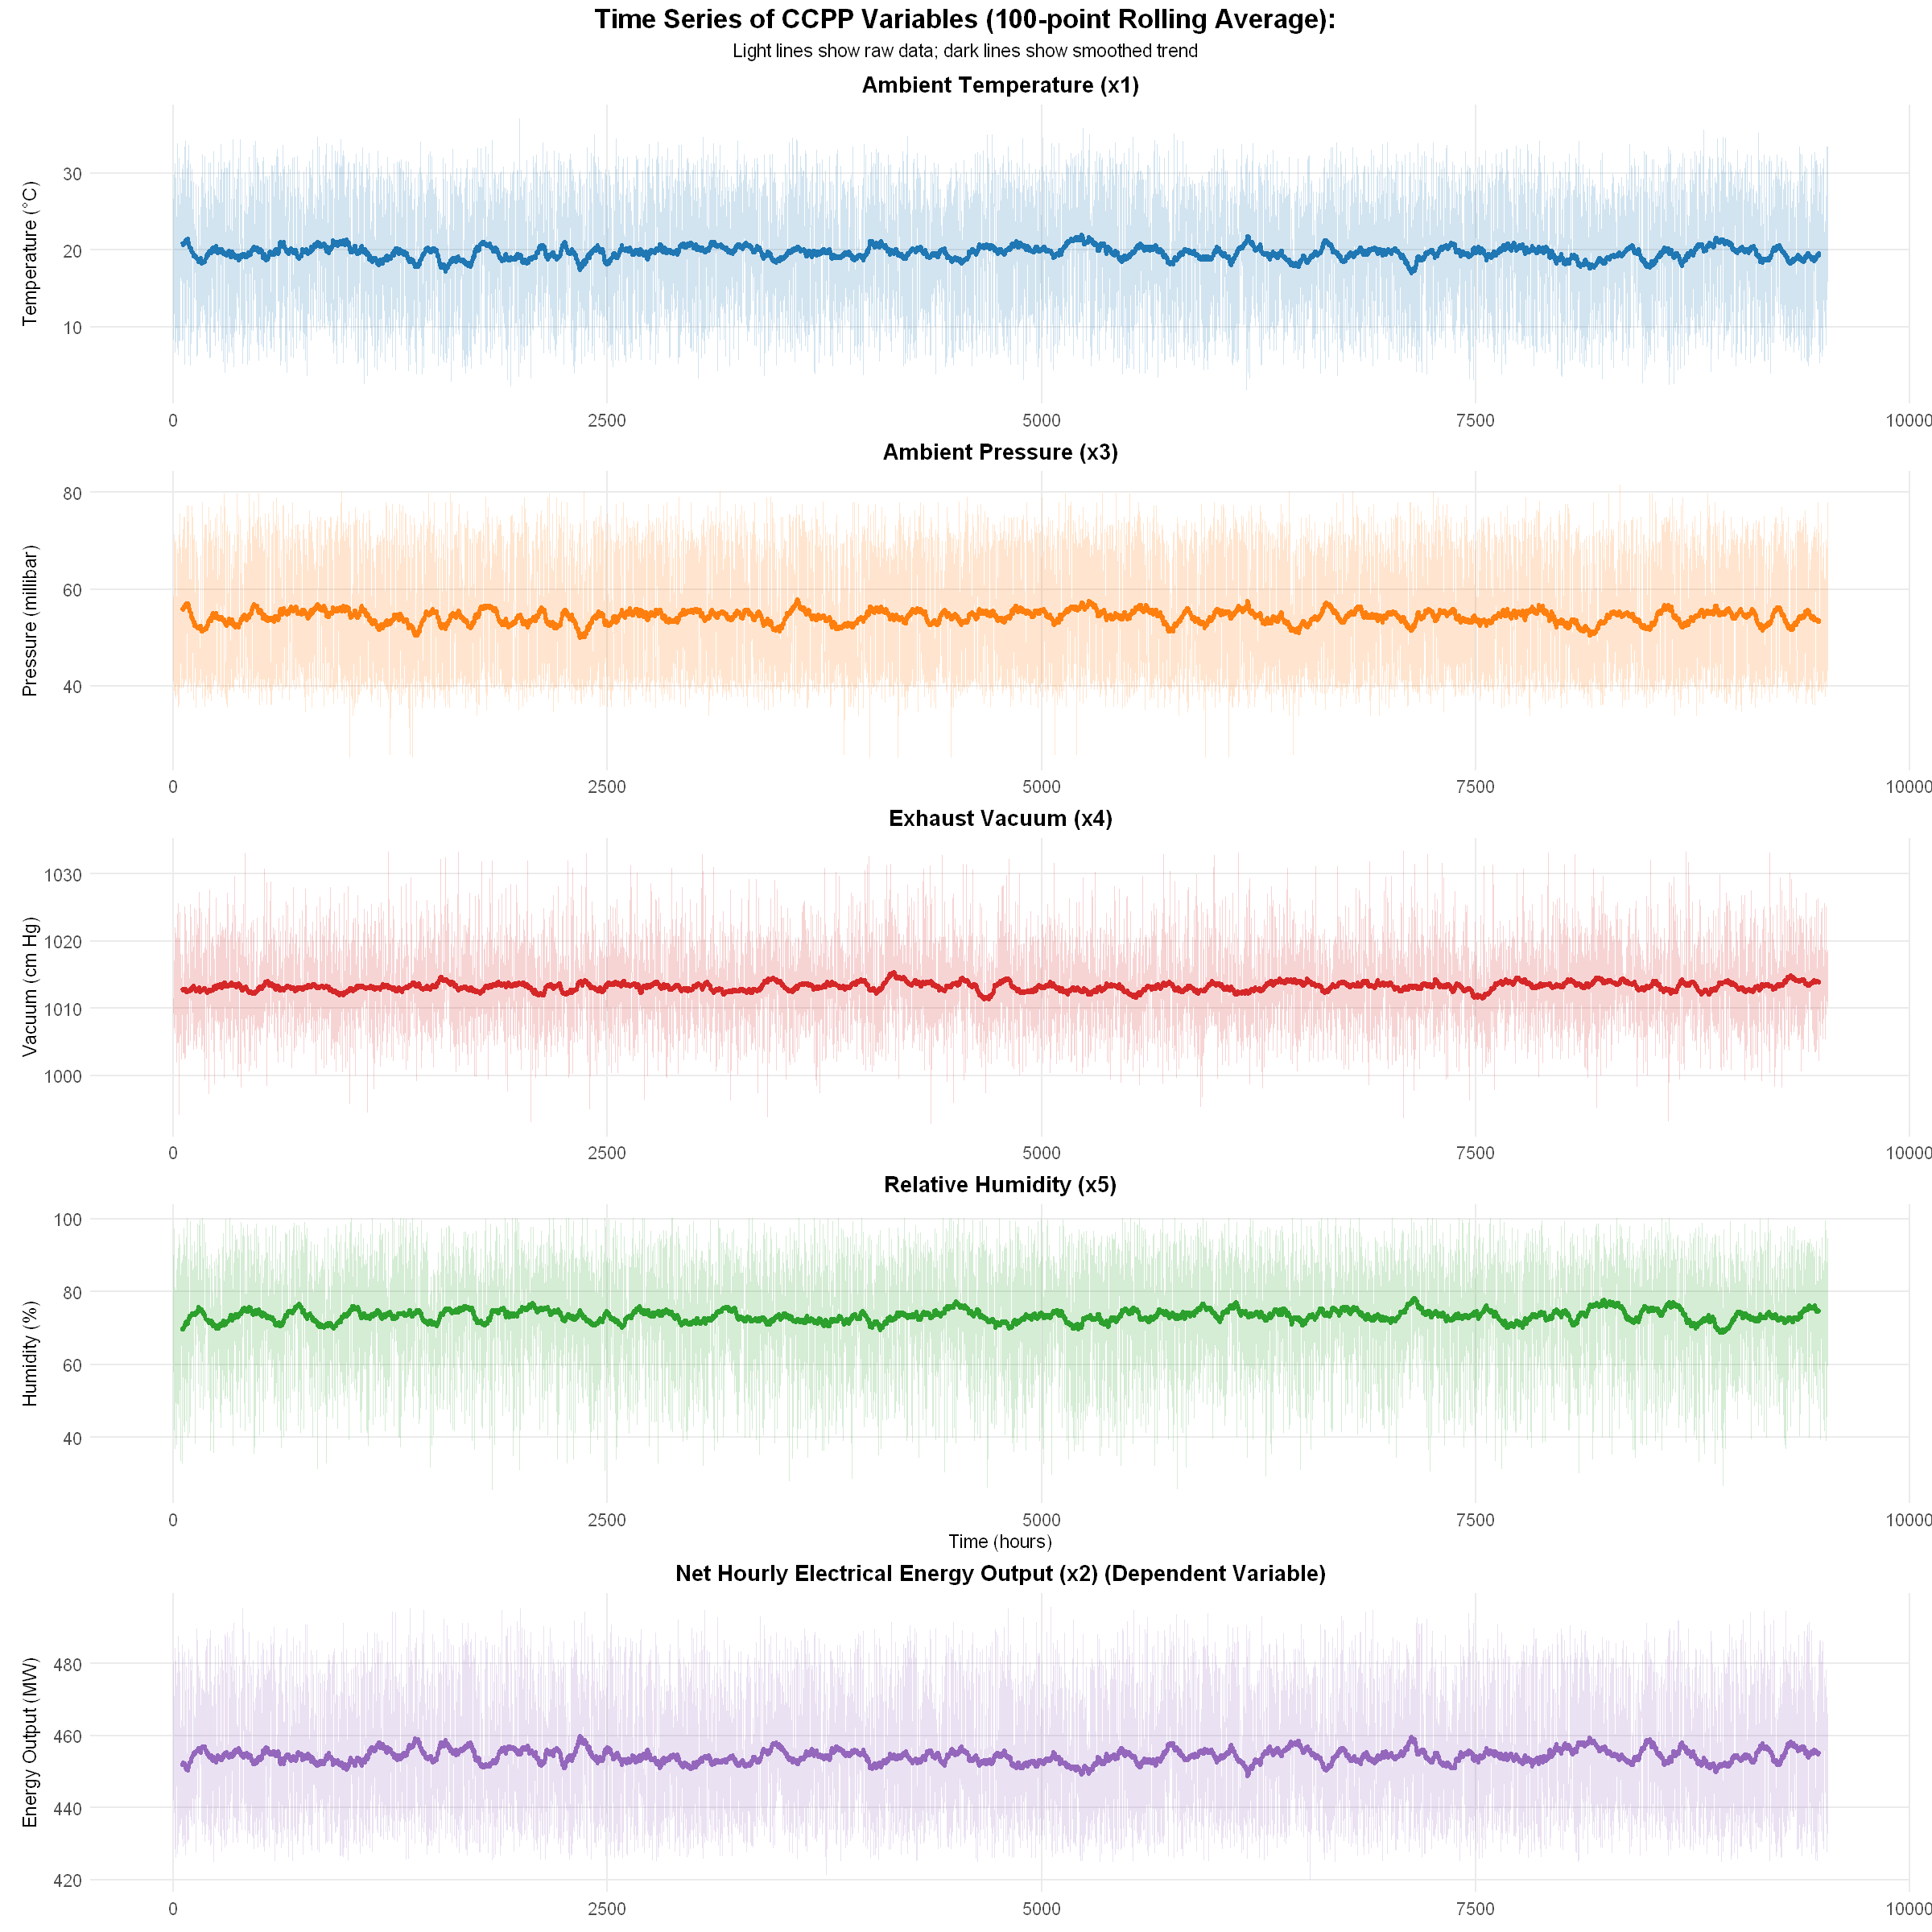
\includegraphics[width=\textwidth]{z4.png}
    \caption{(Time series plots with rolling window of 100 observations)}
    \label{fig:time_series2}
\end{figure}

%\vspace{1em}

The smothing rolling average lines in helps better visualize the overall trends 
but still high clutter is present. %which makes hard to clearly interpret any trends.
To get a more simplified and high-level view of how these variables 
behave over time, the dataset was divided into segments, 
where each segment contains 200 consecutive observations. 
The average of each segment was then calculated and plotted, 
resulting in a cleaner and more interpretable visualization. 

\begin{figure}[H]
    \centering
    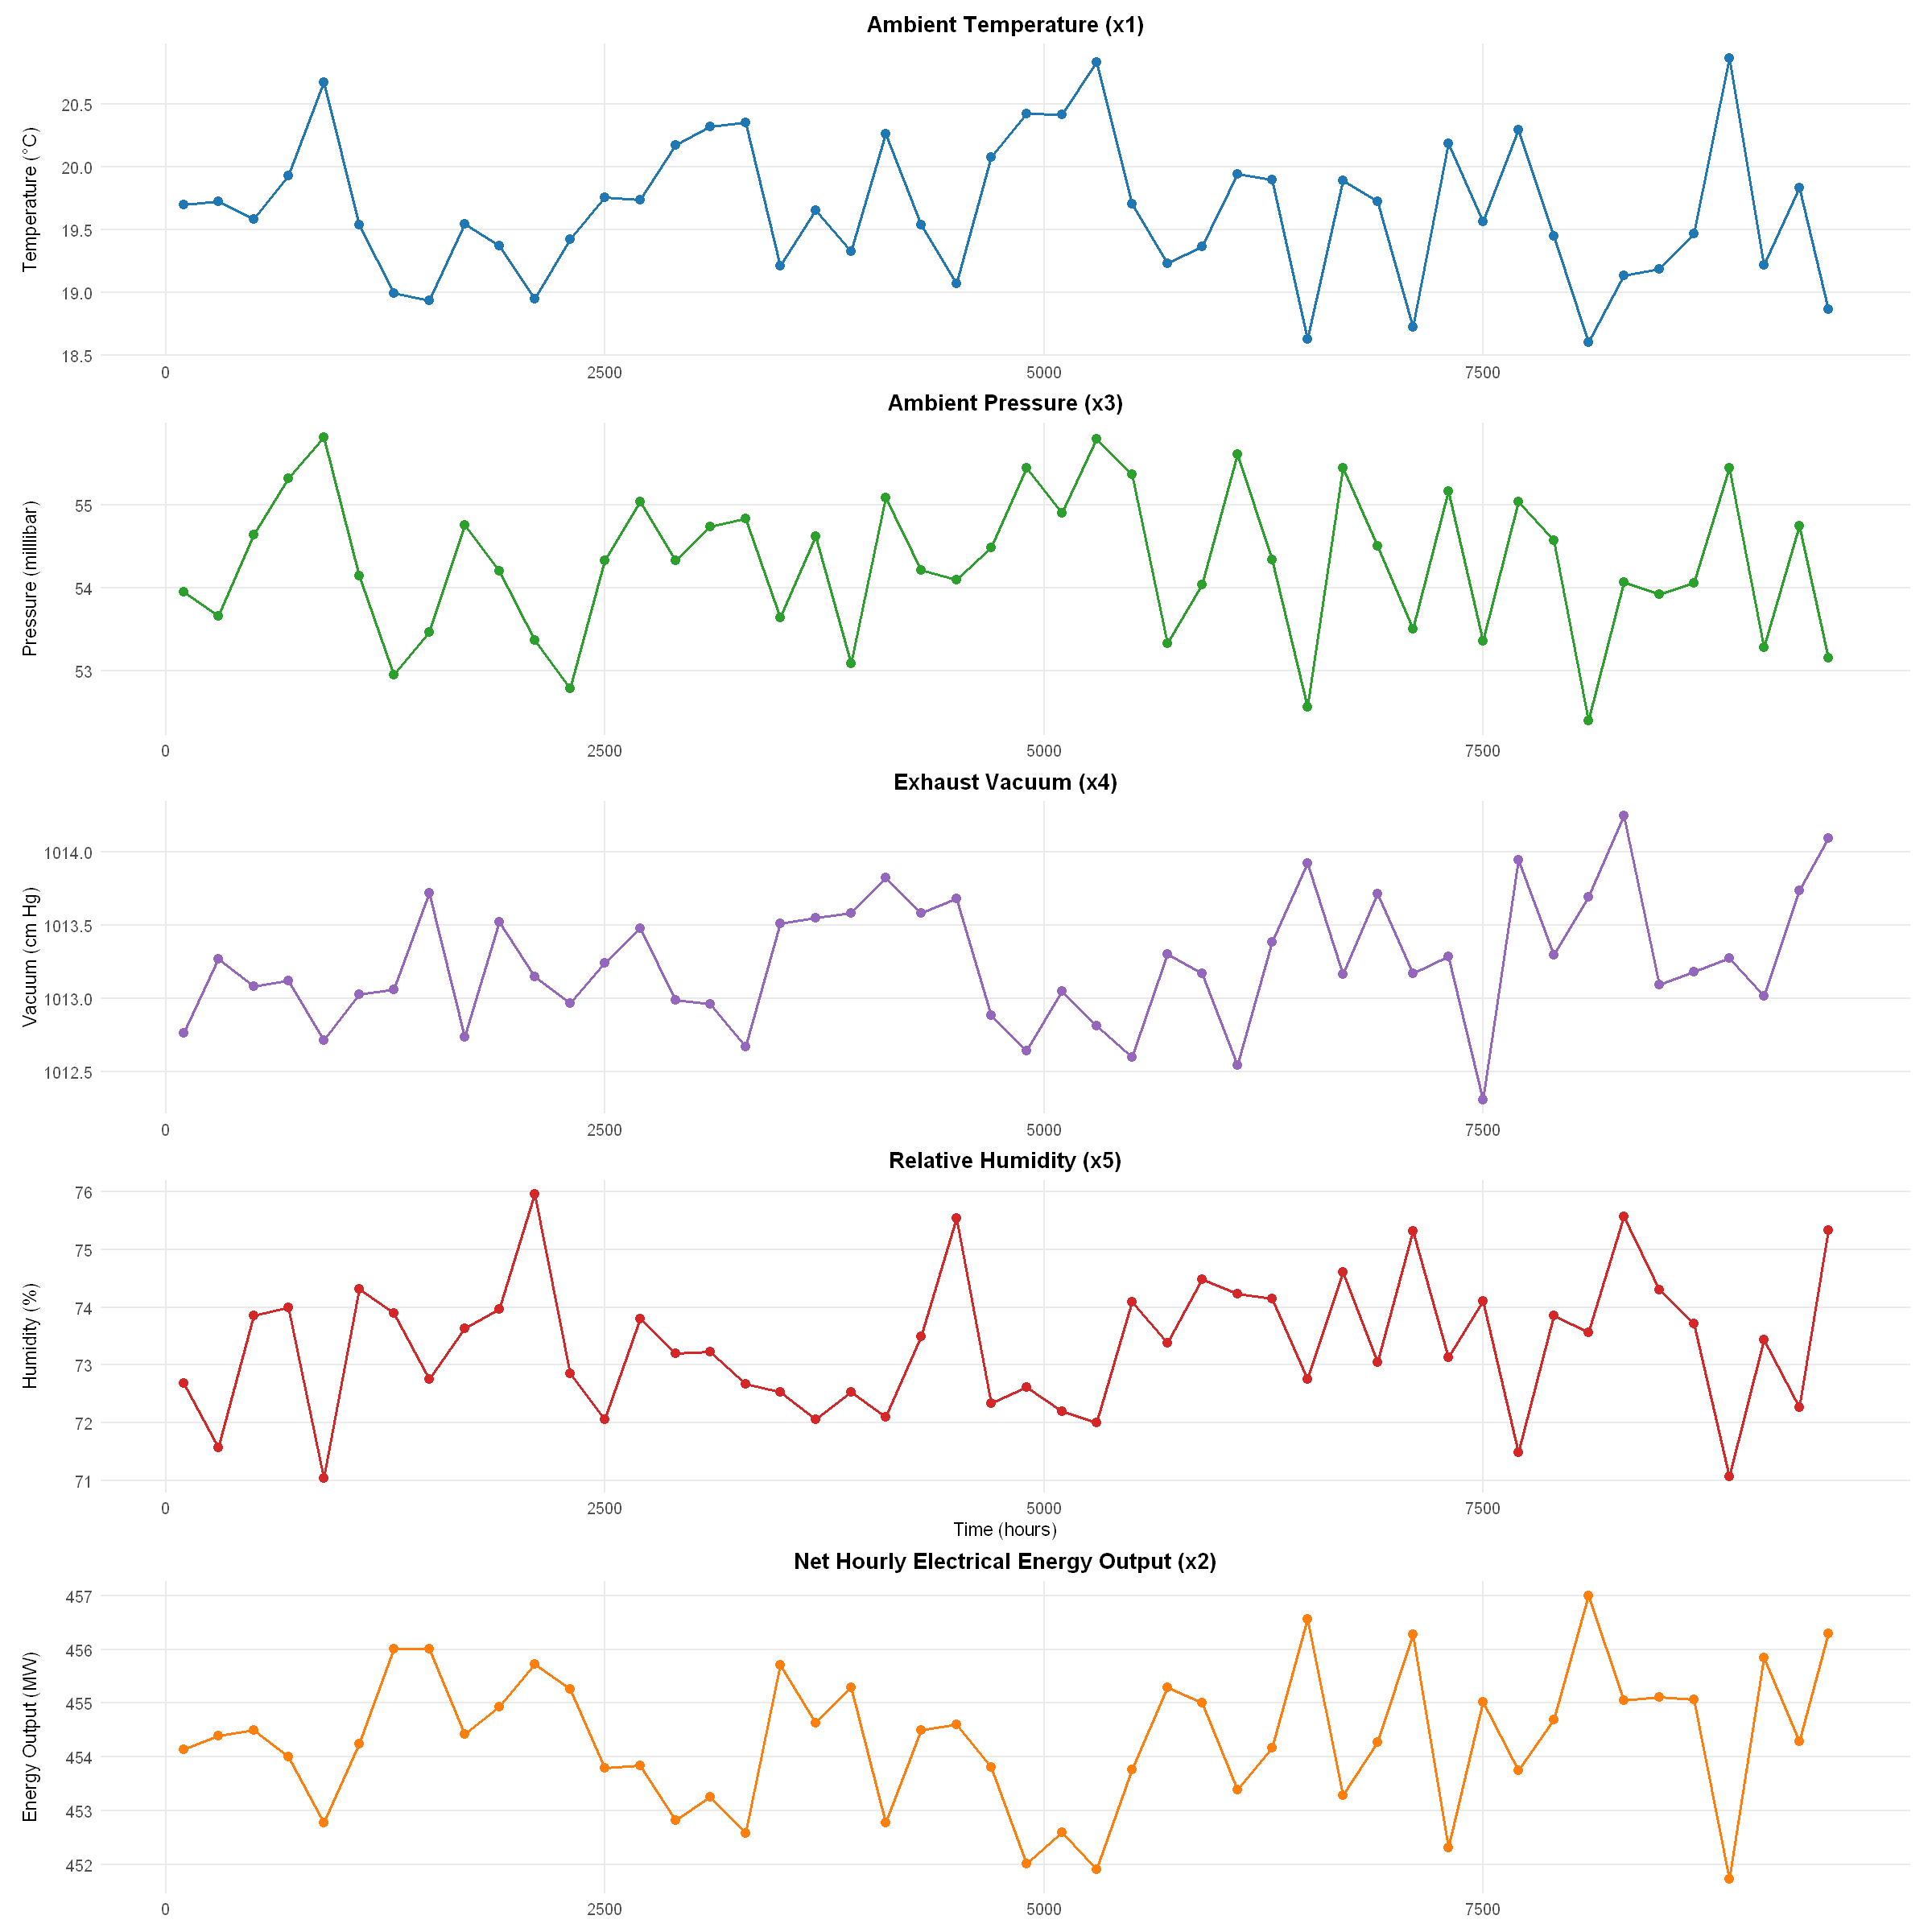
\includegraphics[width=\textwidth]{z5.png}
    \caption{(Time series plots with 200 samples segmentation)}
    \label{fig:time_series3}
\end{figure}

Figure-3 provides a much clear view of the overall trends where 
data is segmented and plotted, rather than plotting every single point.
The ambient temperature (\(x_1\)) shows a strong seasonal trend with mean temprature of $19.66$ degree celcius, with 
regular peaks and dips which reflacts yearly weather changes. Exhaust vaccum 
(\(x_4\)) also shows consistent changes over time ranging from $990$ cmg to $1140$ cm-hg with mean of about 
$1013$ cm-hg, which may be related to other environmental conditions.
Ambient pressure (\(x_3\)) is relatively stable having mean of $54.29$ millibar,  it may indicates 
less influence on energy output. The energy output (\(x_2\)) itself also fluctuates, it is likely due to 
the combined effect of all these variables.

%----------------Distribution Plots-------------
\subsection*{Task 1.3: Distribution Analysis}

Histogram is a type of bar chart where data is divided into different segments called bins or buckets
and shows how many of the observations fall into each bin. If more data points are concentrated
in cretain binning range then this leads to taller bars whereas short bart will be the result of
very few observation into that interval. They helps in identifying unusual patterns in the dataset. 
%Histograms helps in visuallizing general pattern
%of observations in the dataset. 

Density curves, also called kernal density curves are the smoothened version for histograms.
Total area under the density curve is always one representing the whole dataset. The shape
of the curve defines the distribution of valaues within the dataset. 

\begin{figure}[H]
  \centering
  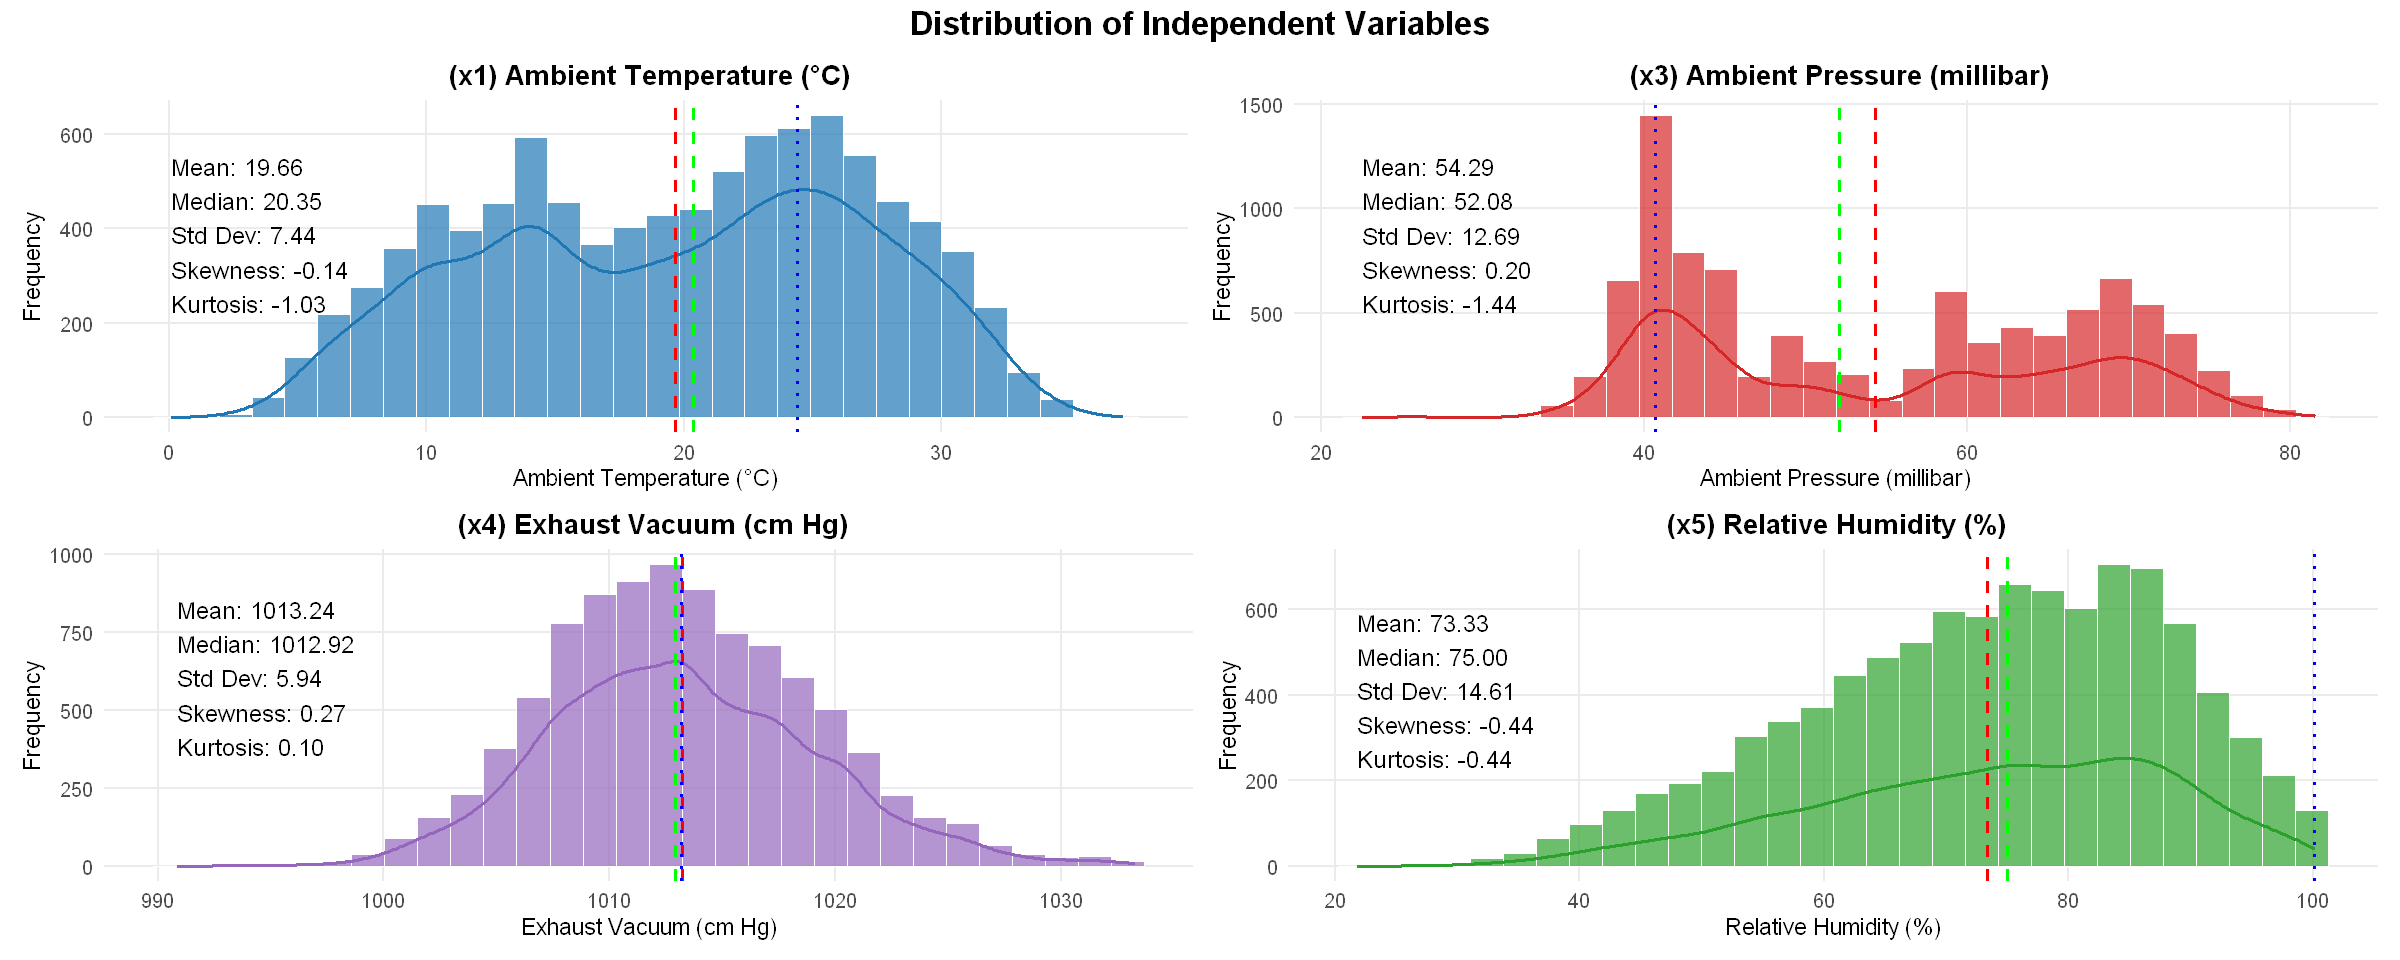
\includegraphics[width=\textwidth]{z6.png}
  \caption{(Distribution of Independent Variables)}
  \label{fig:Distribution of Independent Variables}
\end{figure}

%Figure~4 displays the distribution of each independent variable using 
%histograms combined with density plots. X-axis represents the actual values whereas the y-axis 
%shows the frequency of the observations. Three vertical lines shows the mean(blue), median(green)
%and mode(red dashed) for the distribution of each independent variable.

Ambient Temperature ($x1$) and Relative Humidity ($x3$) show 
slight left skewness ($skewness= -0.14$ and $-0.44$ respectively), which means more values lies along the longer 
tail on the left side. Ambient Pressure ($x3$) shows high variability ($mean= 54.29$, $skewnwss= 0.20$) without approaching to any of the well known
symmetry patterns. Exhaust Vaccum ($x4$) is nearly normally distributed ($mean= 1013.24$, $skewness= 0.27$) showing very little right skewness. 

\begin{figure}[H]
  \centering
  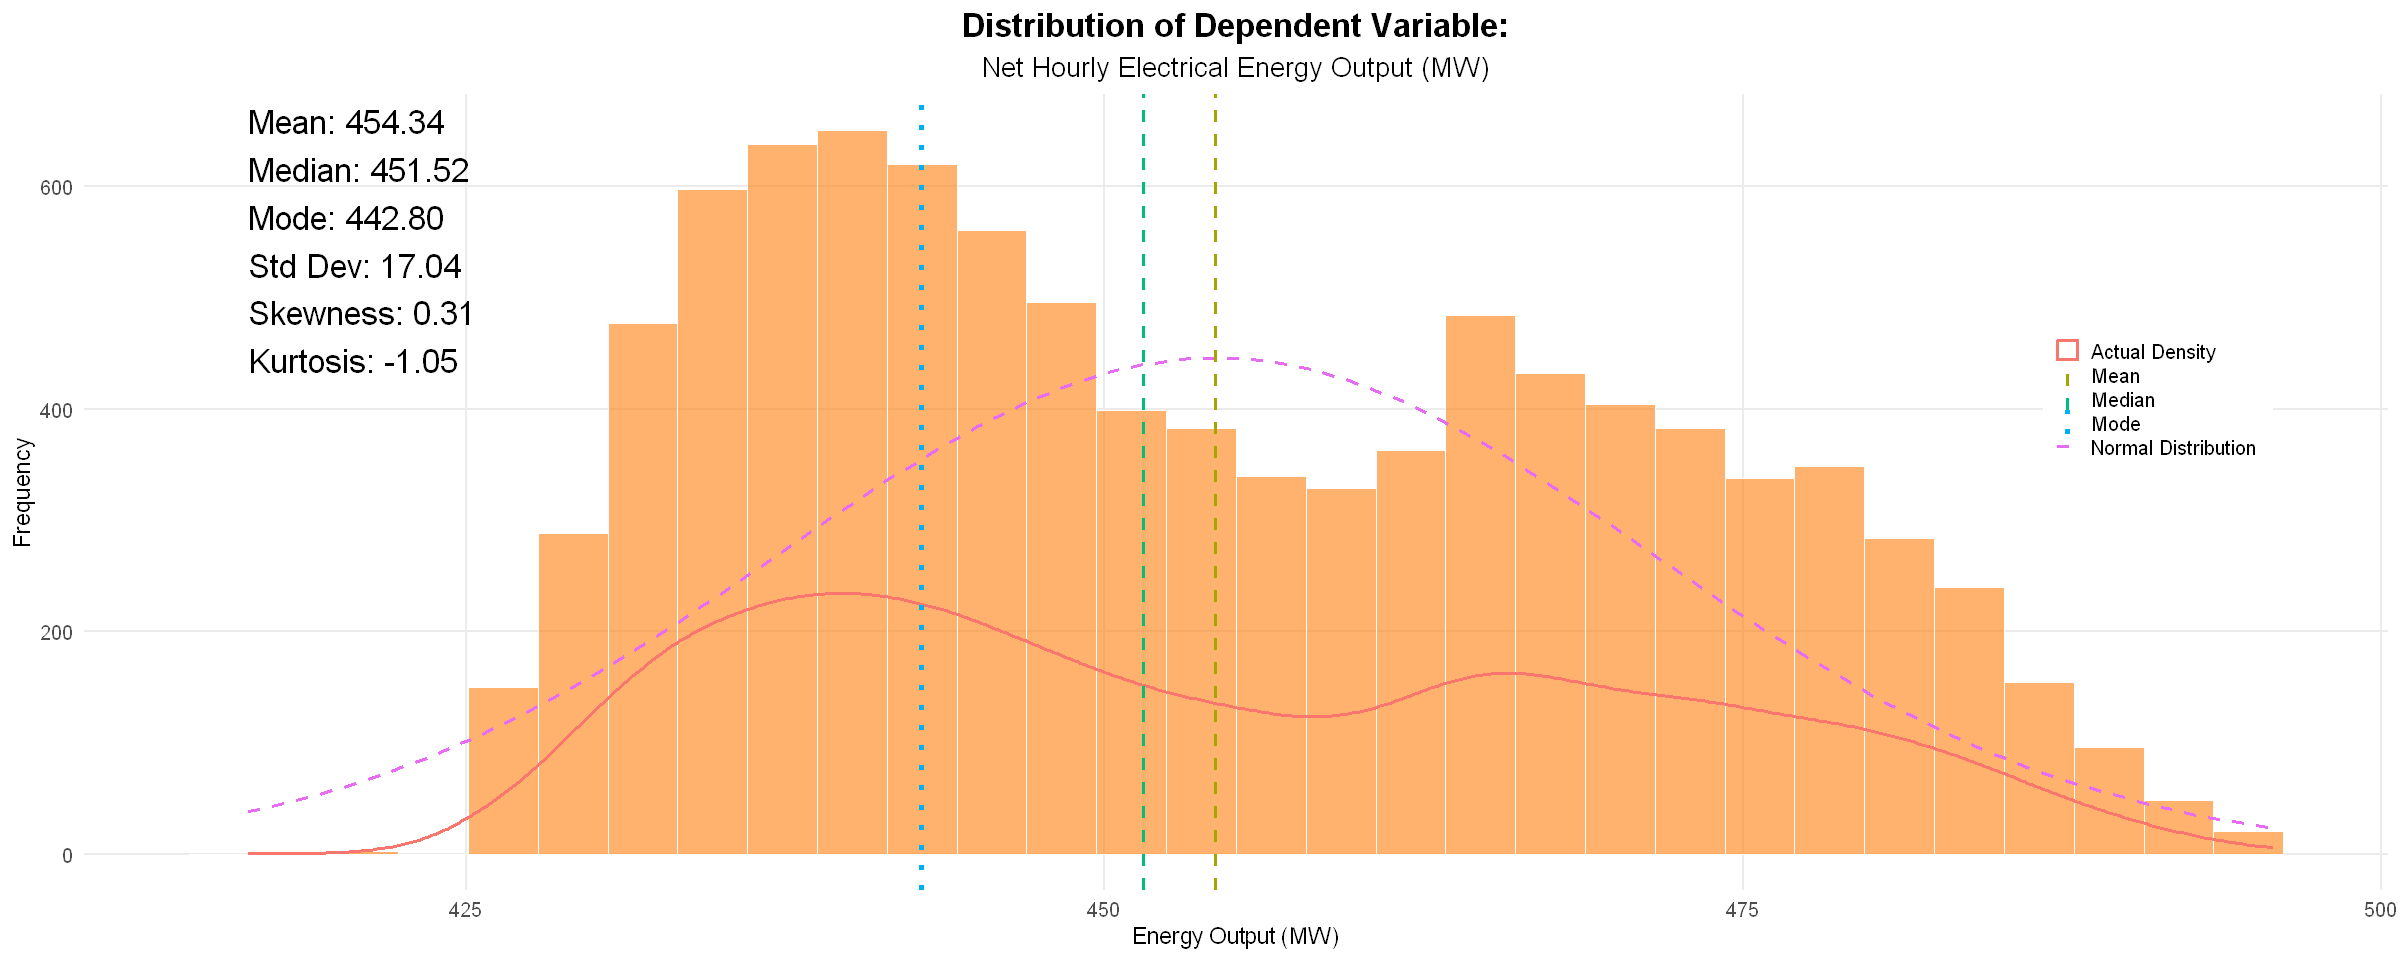
\includegraphics[width=\textwidth]{z7.png}
  \caption{(Distribution energy output)}
  \label{fig:Distribution plot for Dependent Variable ($x_2$)}
\end{figure}

Figure- 5 shows the distribution of the dependent variable, net energy output ($x2$) `MW`. 
The distribution for energy output
is slightly right-skewed, where most values are in between 
$430 MW$ and $470 MW$. The mean energy output is about $454 MW$ whereas 
median is sligtly lower at around $451 MW$ which is an indication of slight right skewness. 
The standard deviation of about $17 MW$ also indicates moderate variability in 
the enorgy output. 

%----------------Normality of Data-----------------------

\subsection*{Task 1.4: Normality of Data}

Q-Q plot, or Quantile-Quantile plot, is a plot used to check  
whether a dataset follows a particular theoretical distribution; most 
commonly, the normal distribution. It works by comparing the quantiles of dataset we have to the 
quantiles of the normal distribution. 

To interpret a Q-Q plot, we simply examine how closely the plotted points 
follow the reference line. If the points lie on the reference line or form clusters 
around the line then generally, our data follows normal distribution. If the 
points curve above or below the line then it indictes left or right skewness
and so the data is not symmeteically distributed. If the points form a s-shaped
curve around the line it is an indication of high kurtosis. 

\begin{figure}[H]
  \centering
  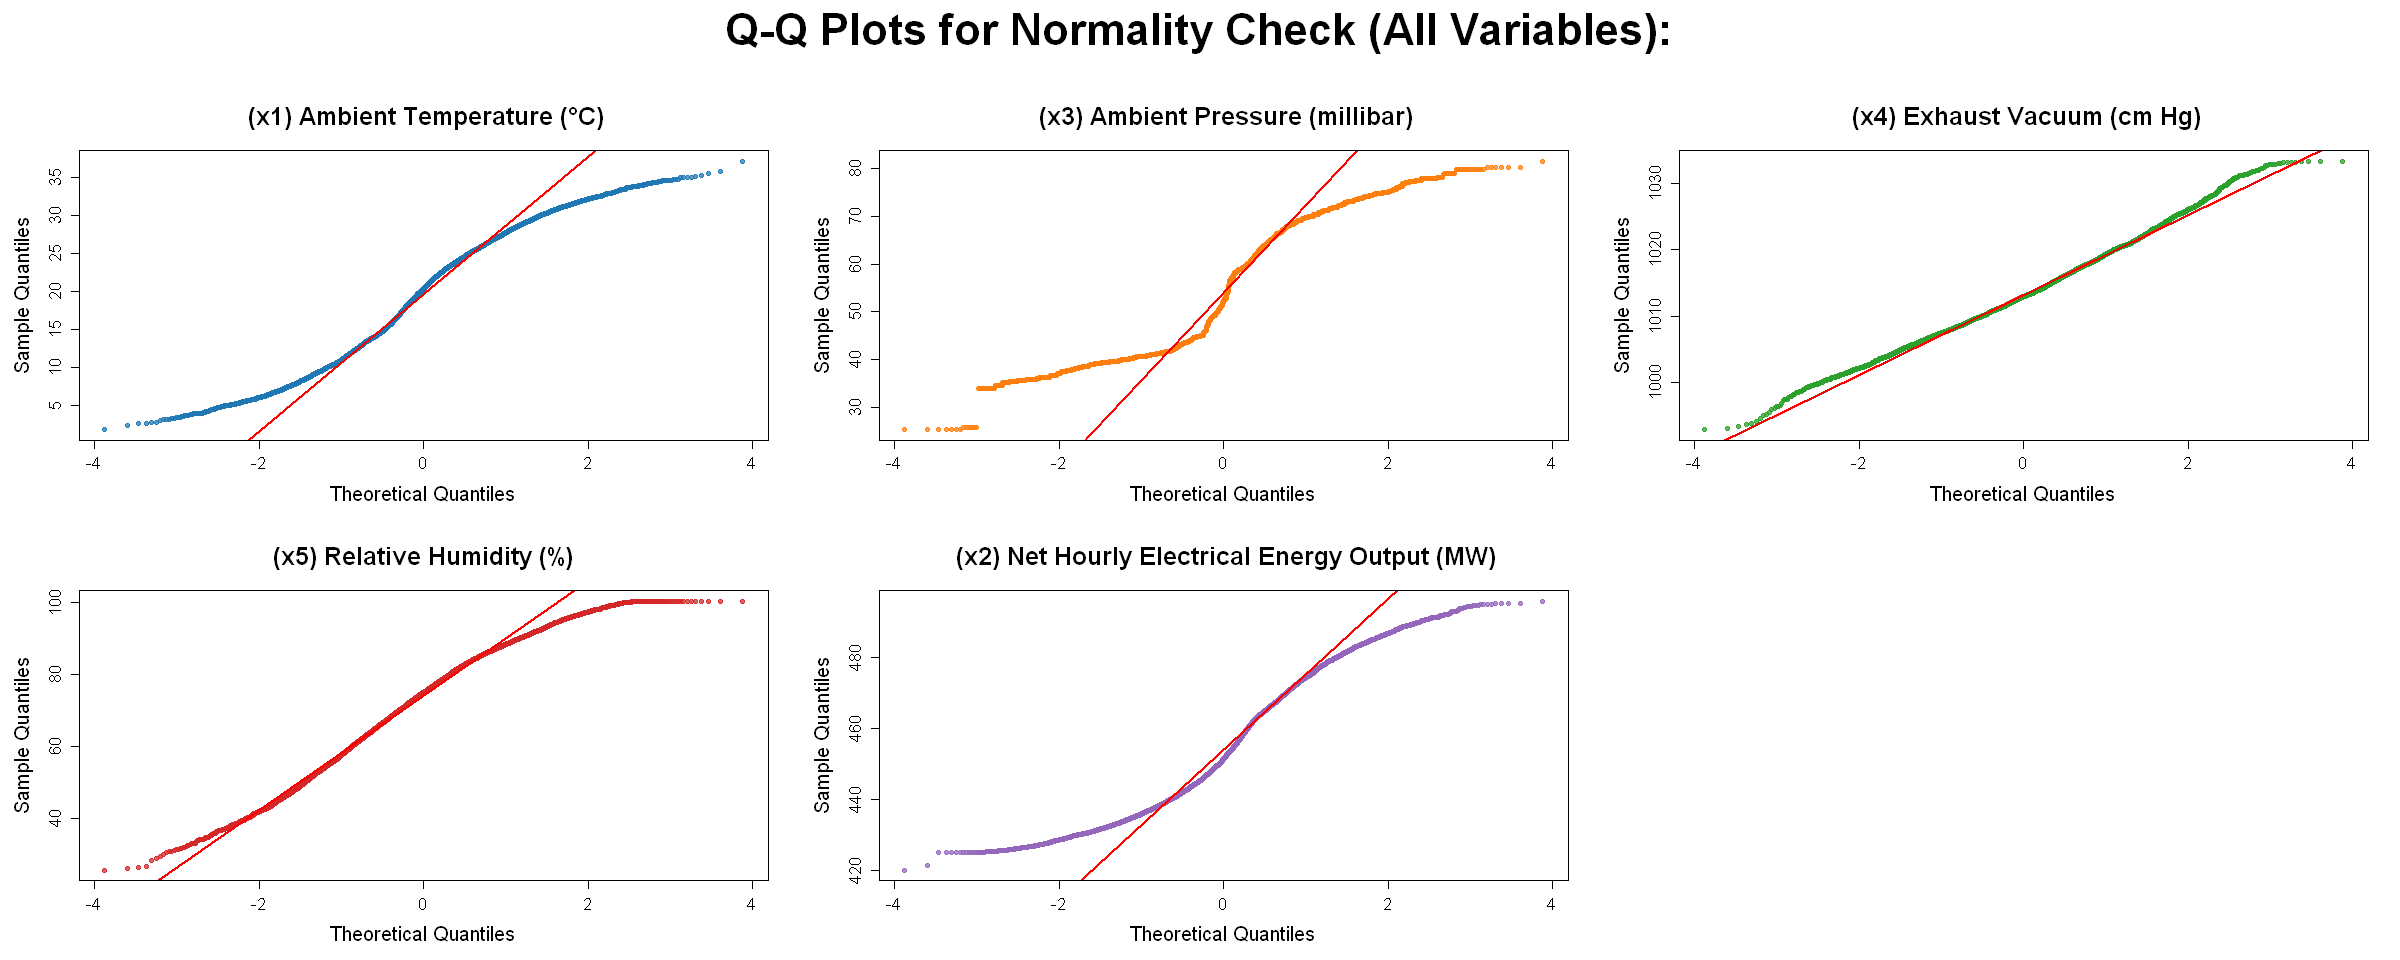
\includegraphics[width=\textwidth]{z8.png}
  \caption{(Normality test for variables)}
  \label{fig:Normality of Data}
\end{figure}

Figure-6 shows, ambient 
temprature ($x1$) and relative humidity ($x5$) shows deviations at both 
tails (clearly visible $S$-$shape$ curves) results in slight deviation from normal distribution. 
Energy output ($x2$) shows a noticeable long tails (clear $s$-$shape$ curve) on both ends. The ambient pressure ($x3$) 
is clearly not normally distributed as it shows very high deviations from the
reference line. Exhaust vaccum ($x4$) aligns very 
closely with the red line, it is mostly normally distributed. 

%----------Outlier Detection------------

\subsection*{Task 1.5: Outliers Detection}
 
The box plot (sometimes also called box-and-whisker plots) shows the spread and summary of data using five 
summary statistics: maximum, first quantile (Q1), median (Q2), third quantile (Q3)
and maximum value. %The box represents the interquartile range IQR (Q3-Q1) and 
%contains middle 50\% data. A line inside the box is the median line. Lines
%that extends from both ends of the boxplot are called whiskers and they extend to 
%the minimum and maximum non-outlier points of the dataset. 

The observstions that fall outside the range (whisker tips on both sides) are the potential outliers.
A large box generally indicates high variability in the data values, one long whisker is an indication
of skewness (right skewness or the right skewness) and a symmetrica box shape represents normality.

A violin plot extends the box plot by showing the 
distribution's shape using kernal density estimation plot. It displays the central tendency,
shape and variability of data in a single plot. More wider sections in the violin plot 
indicates more concentration of observations whereas irregular and multiple dips and valleys 
indicate complex distribution structure.

\begin{figure}[H]
  \centering
  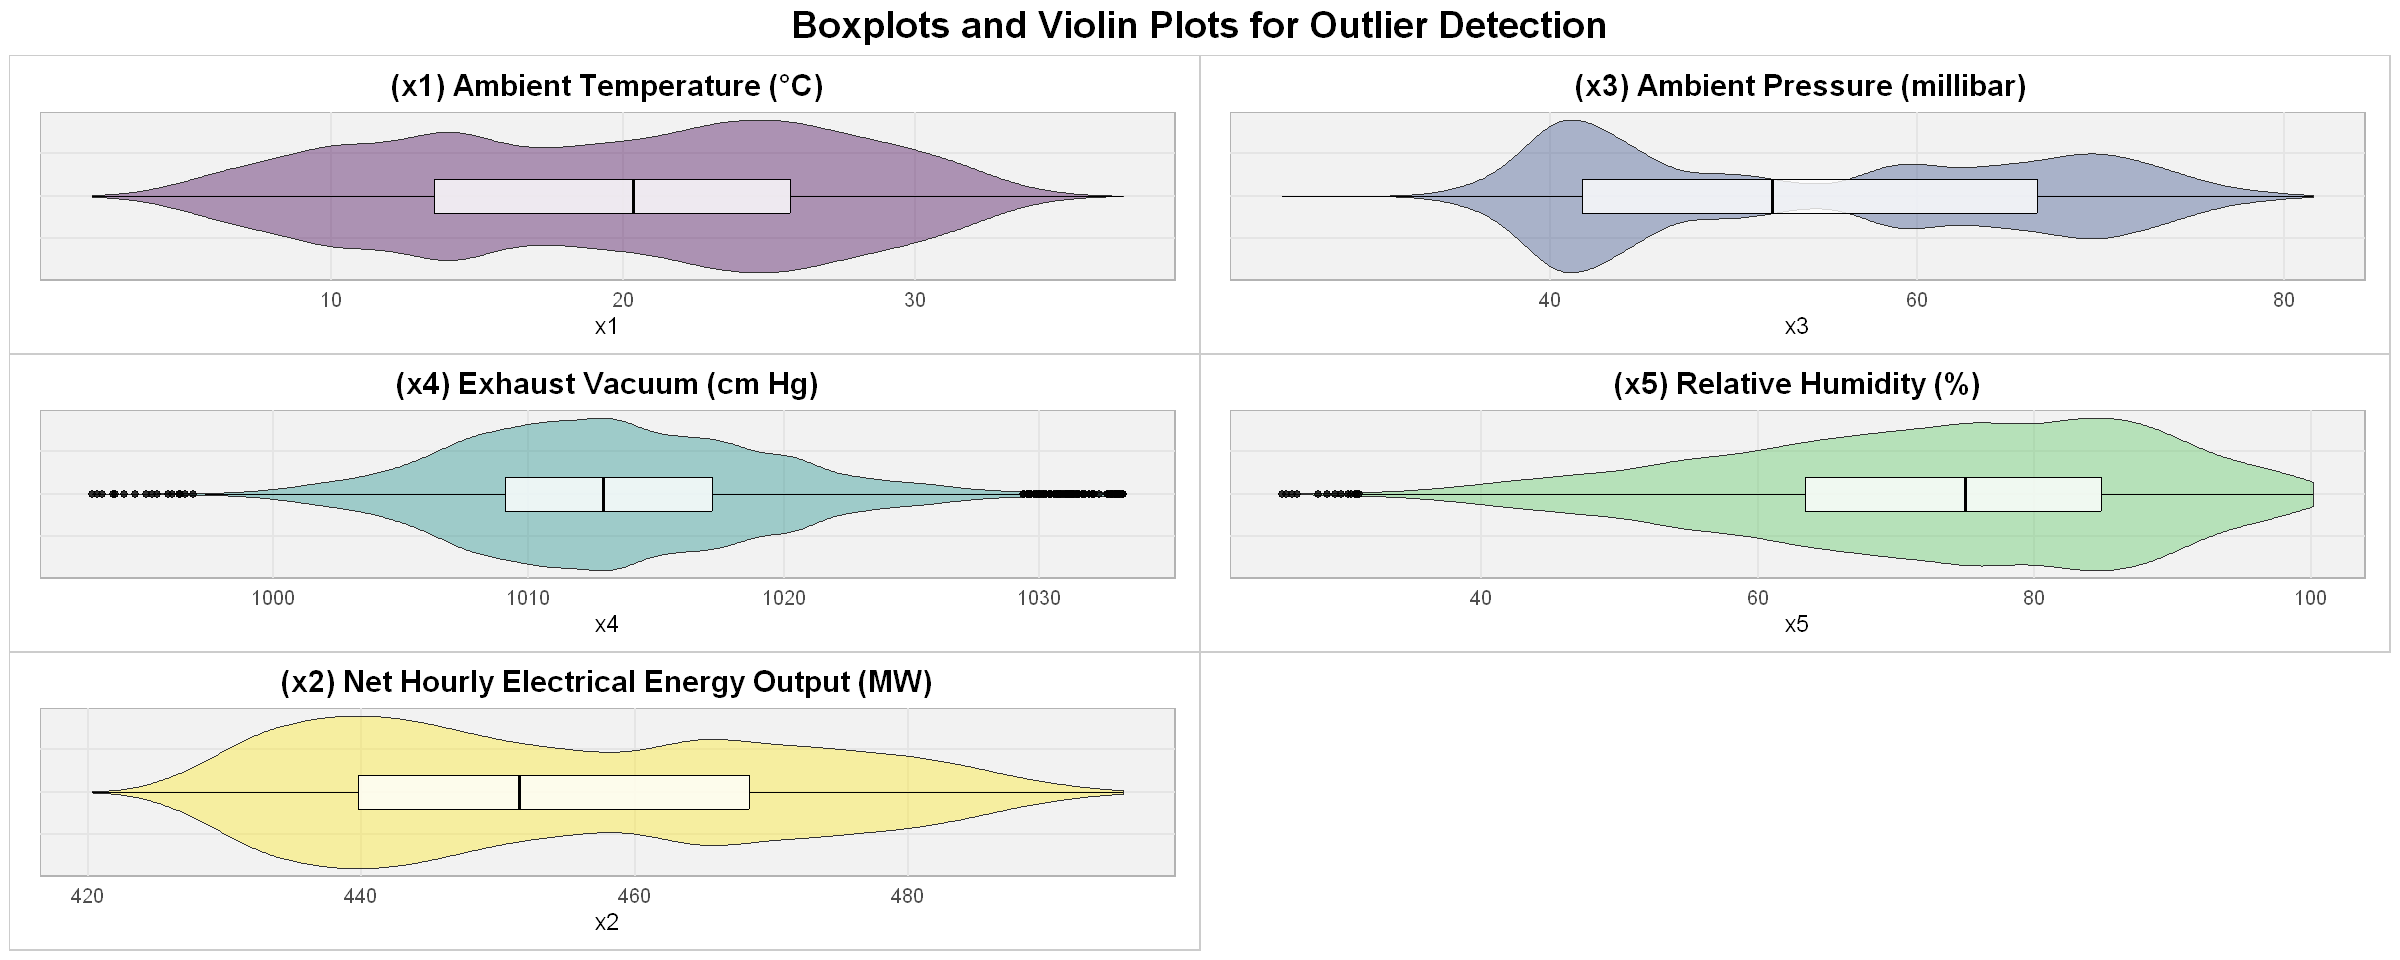
\includegraphics[width=\textwidth]{z9.png}
  \caption{(Box-Violin plots)}
  \label{fig:Outlier Detection}
\end{figure}

From Figure~7; relative humidity ($x5$) have outliers on both tails because dots are present on both ends. 
Exhaust vacuum ($x4$) also shows several outliers along the left-tail which makes it left-skewed. 
Ambient pressure ($x3$) also shows potential outliers on both ends. 
In contrast, ambient temperature ($x1$) and energy output ($x2$) shows 
relatively fewer extreme values. The shape and distribution of ambient pressure ($x3$) is 
complex as the distribution is almost divided into two halfs around median (multimodal distribution). 

%The outliers we've found here shows rare but important poerational conditions. 
%Power plants sometimes face unexpected events that cause 
%extreme values, but these are all valid observations. 
%Including them in the model makes sense as they make the model 
%stronger and more realistic to extreme values.

%-------Scatter Plots----------------------------------

\subsection*{Task 1.6: Scatter Plots and Correlation Analysis}
Scatter plot shows individual data points using dots in a 2D plot. Each dot represent 
a pair of values for two variables $(x,y)$. %The independent variable is generally plotted 
%along x-axis and the dependent or resulting variable is plotted along y-axis. 
To interpret the 
relation, we look for the trend of points like; dots go up from left to right (up-trend),
dots go down from right to left (down-trend), dots scattered randomly indictes weak or 
no relationship between variables. If the points shape into some curve like patterns then
it is an indication of non-linear relation or higher-order relation.

Correlation is a way to measure how two variables are related 
considering all other variables constant. It shows whether an increase
in value of one variable is associated with the change in values of other variable.

For correlations between independent and dependent variables 
(like temperature ($x1$) and energy output ($x2$)), stronger correlations 
are beneficial. However, strong correlations between independent 
variables can create a challenge called multicollinearity
(when predictor variables are highly correlated with each other).

\begin{figure}[H]
  \centering
  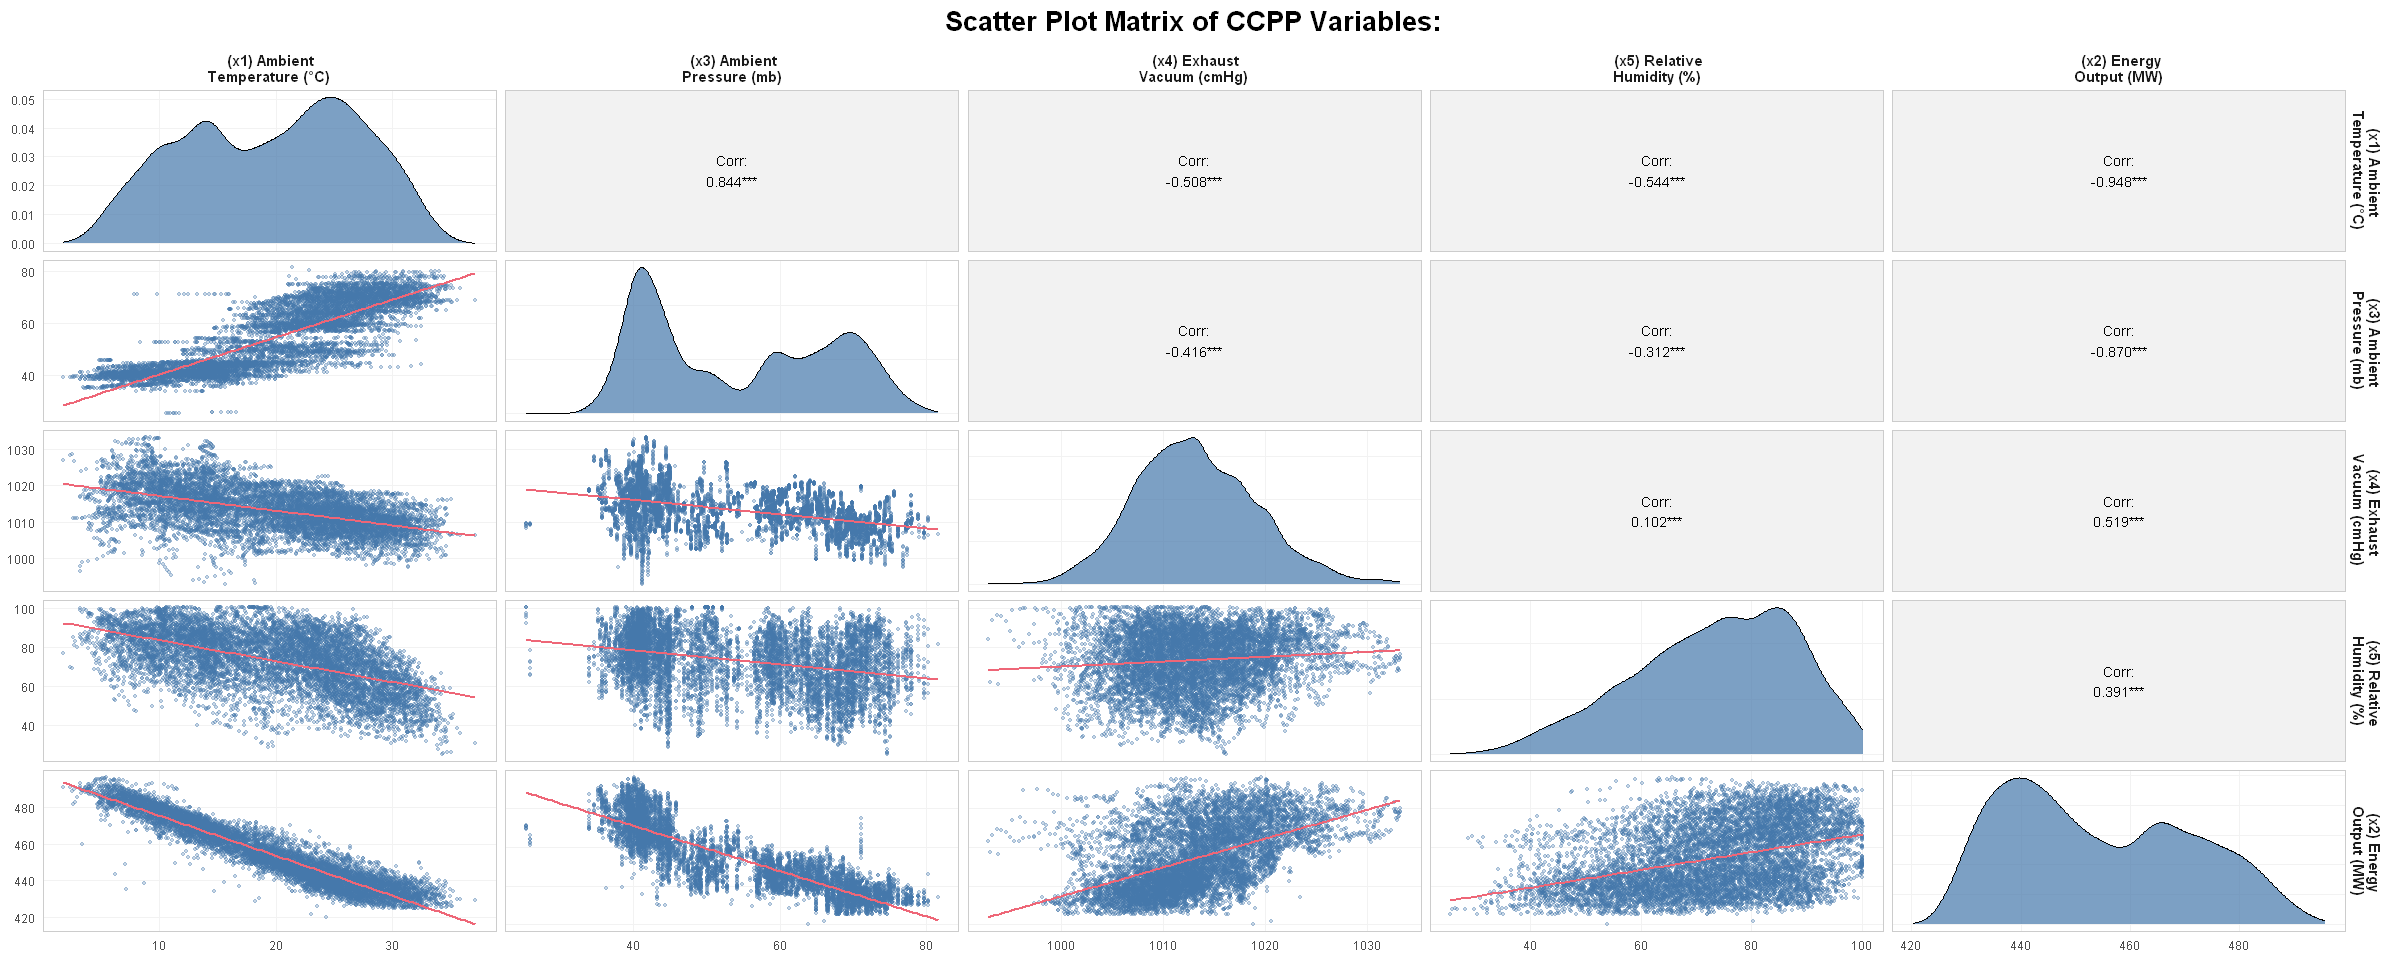
\includegraphics[width=\textwidth]{z10.png}
  \caption{(Scatter plots of all variable combination where, diagonal cells represent density plot for each variable)}
  \label{fig:Scatter Plot}
\end{figure}

In above figure, some environmental factors shows a strong link with 
energy output. Temperature ($x1$) have a strong 
negative relationship with energy output (monotonic relation) meaning, increase in one values (temperature) results in decrease in the value of other (energy). 
Ambient pressure ($x3$) also have a strong relationship with energy ($x2$), and high vacuum ($x4$) inside the chamber generally leads to 
more energy output (a rule from Thermodynamics). The relation between humidity ($x5$) and energy output ($x2$) is moderate so the 
influence of humidity is not that noticable compared to effects of temperature and vaccum.
The diagonal cells represent the distribution of each variable using kernal density estimation (kde). Temprature ($x1$) and ambient pressure ($x3$)
may be multimodal as indicated by multiple peaks. 

%----------------Correlation and Scatter Plots-------------
Pearson's Correlation analysis was performed to further justify the relation between 
variables and resulting correlations are recorded on the following heatmap:

\begin{figure}[H]
  \centering
  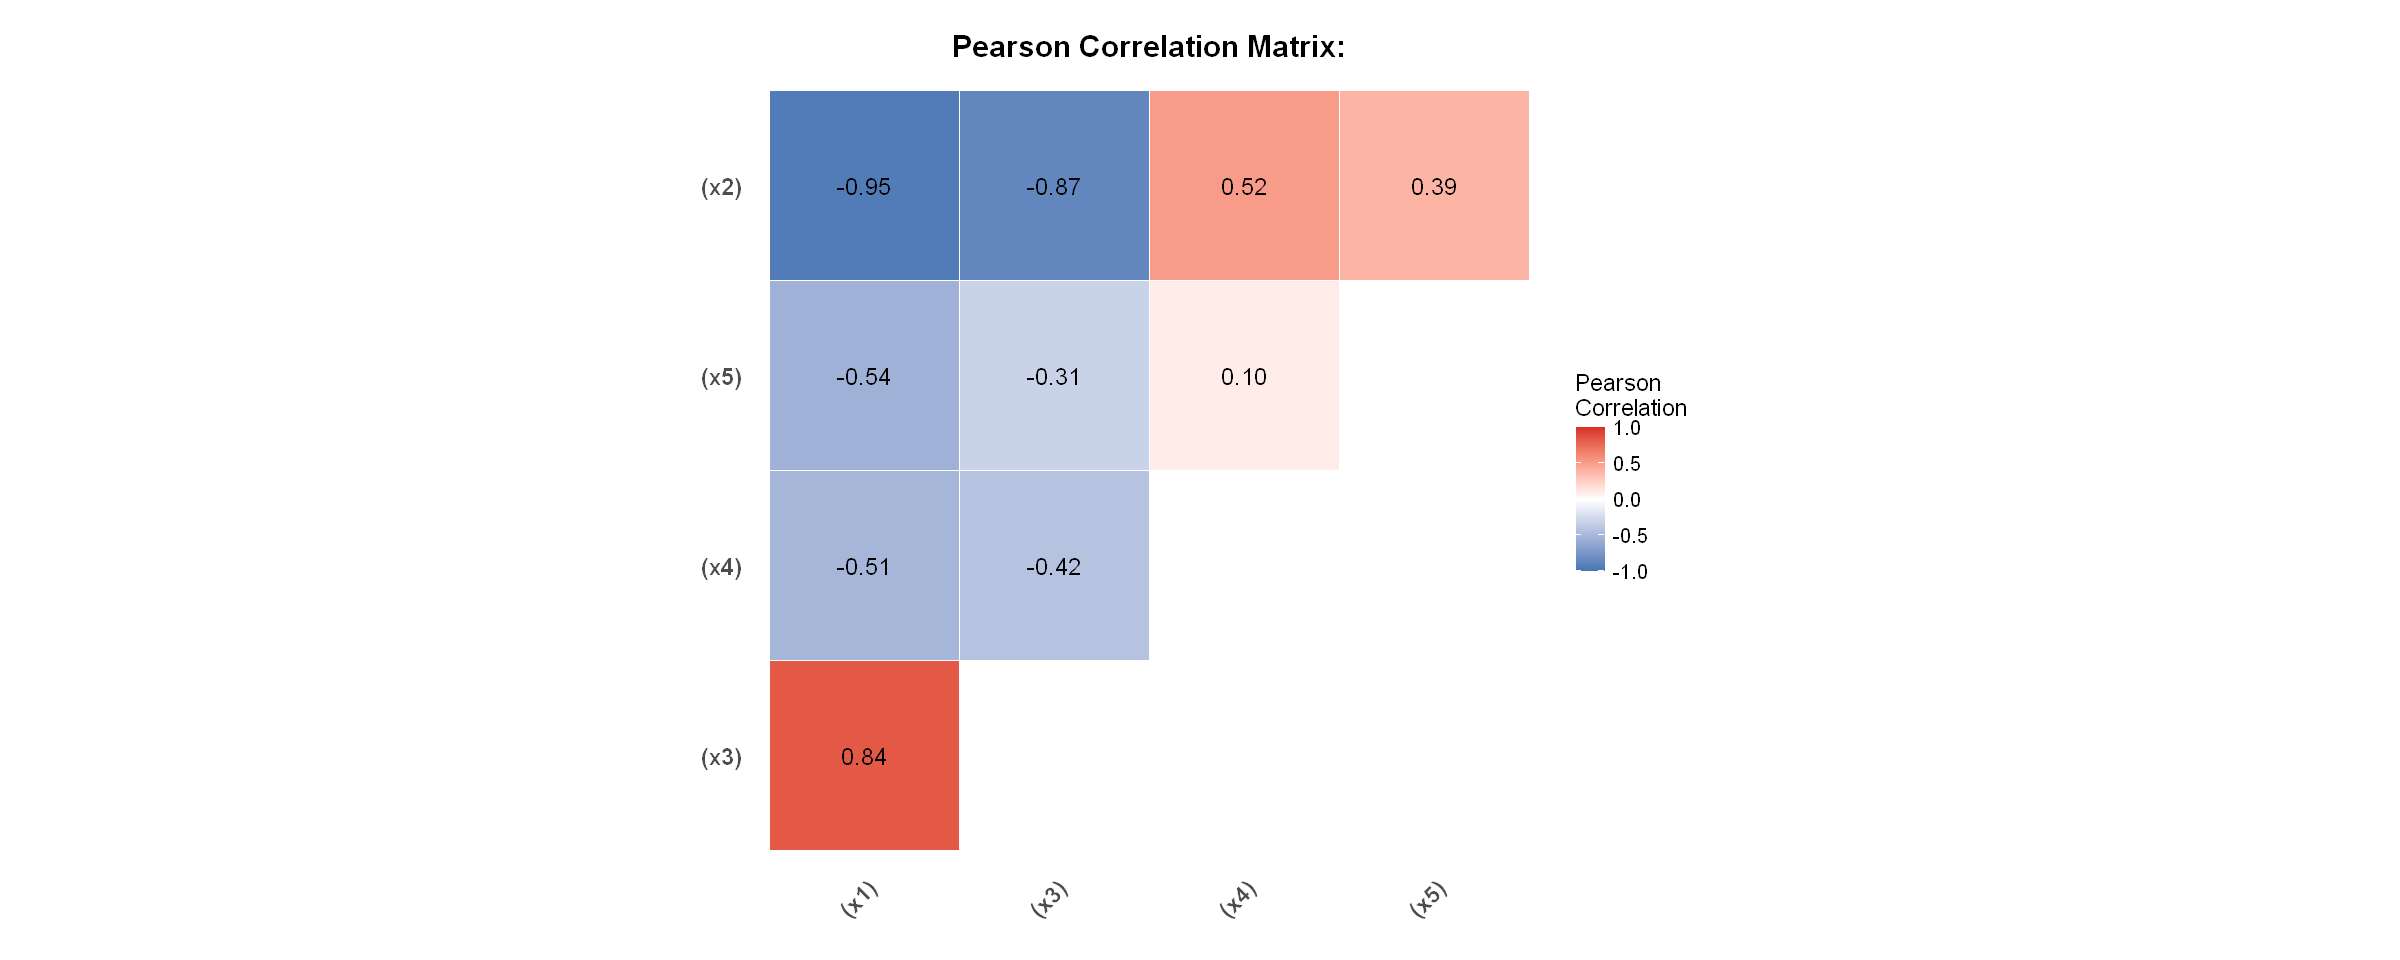
\includegraphics[width=\textwidth]{z11.png}
  \caption{(Pearson's Correlation heatmap between different variables)}
  \label{fig:Pearson Correlation Matrix}
\end{figure}

To better capture the monotonic relation between variables, Spearman's 
Rank Correlation analysis was performed and the resulting coefficients are 
recorded in the following heatmap: 

\begin{figure}[H]
  \centering
  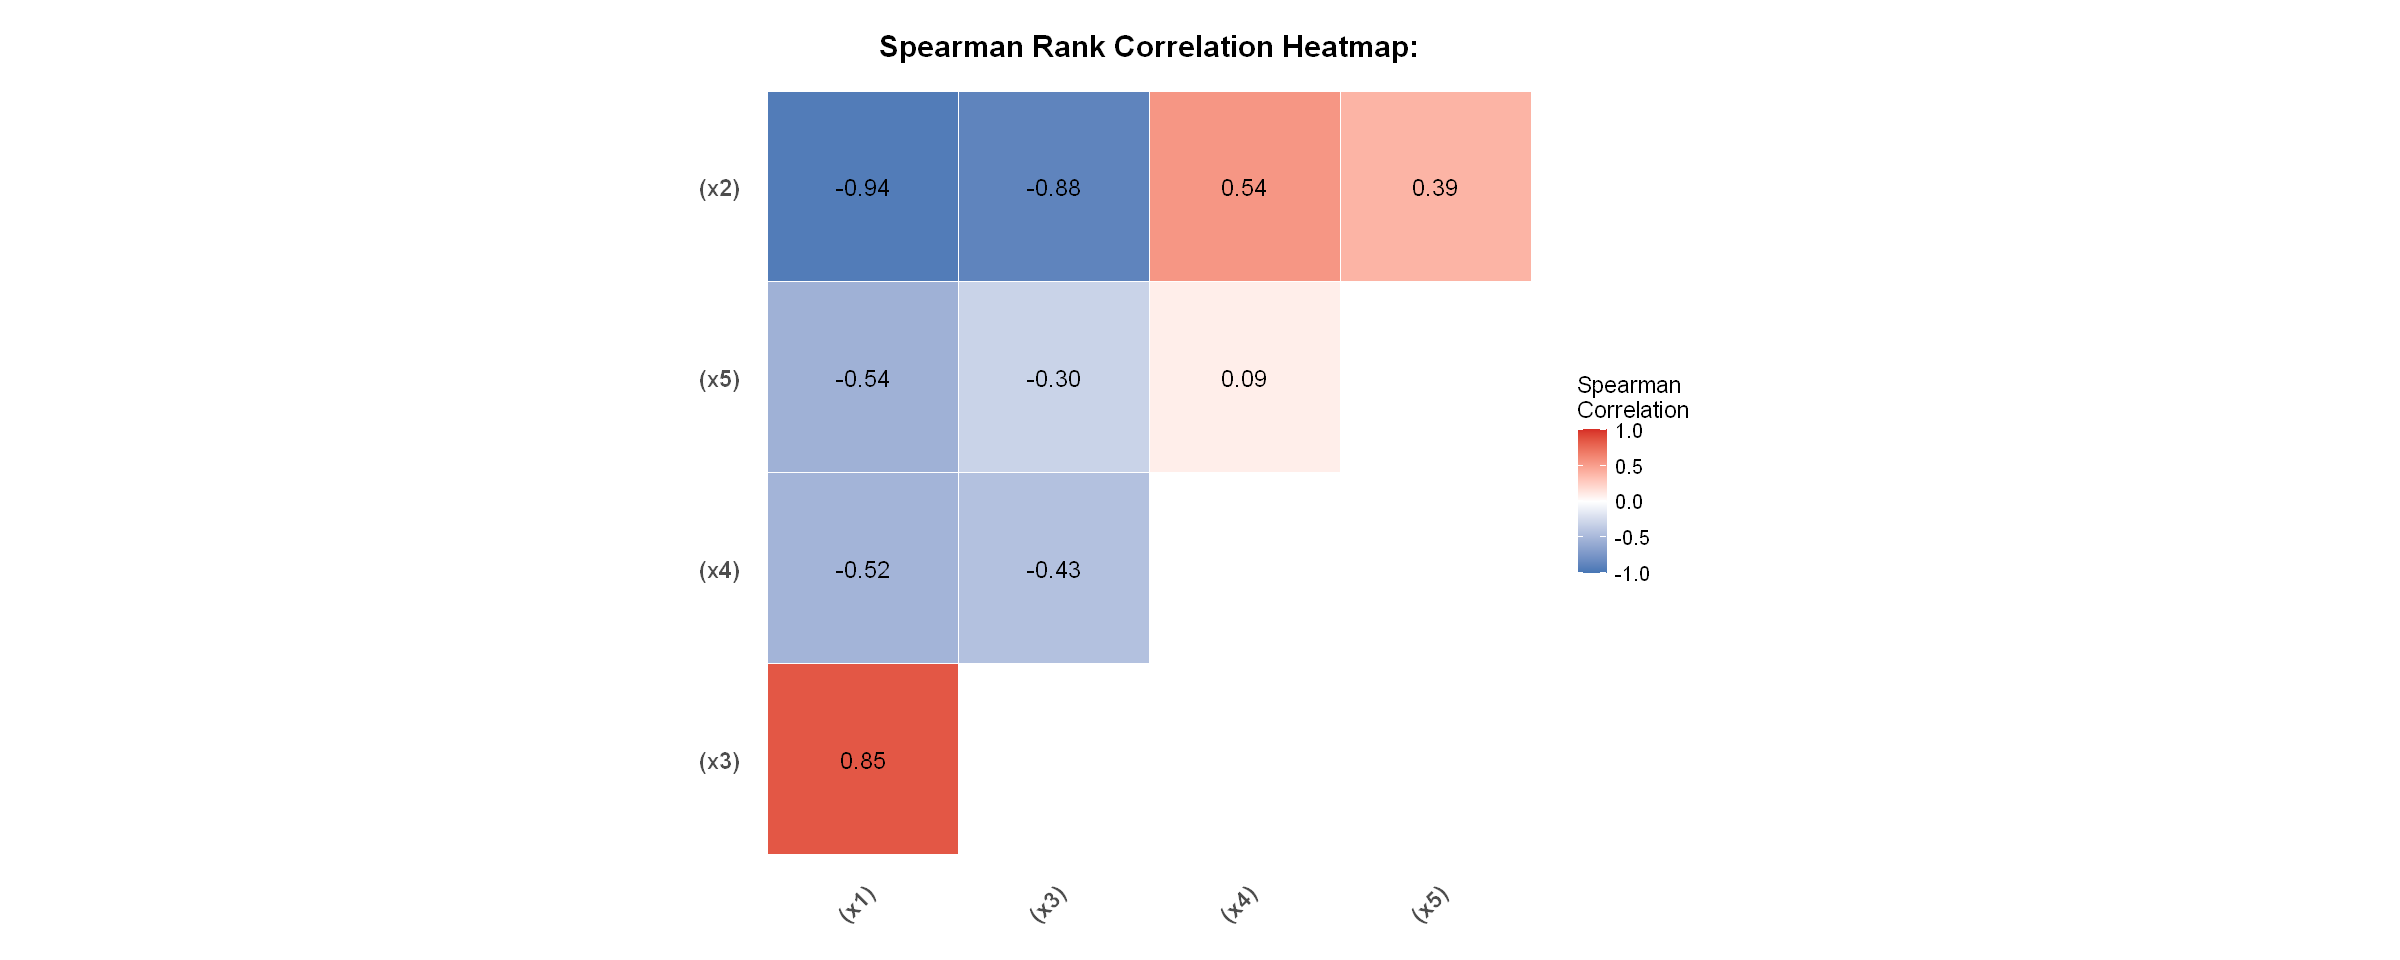
\includegraphics[width=\textwidth]{z12.png}
  \caption{(Spearman's Rank Correlation heatmap between different variables)}
  \label{fig:Spearman Correlation Matrix}
\end{figure}

A very correlation ($\text{Corr} = -0.94$) is observed between temperature ($x_1$) and output ($x_2$)
, so generally as one value (like ($x_1$) increases), the other variable value $x_2$ consistently 
decreases in a monotonic fashion. So, temperature becomes one of the 
most influential factors affecting energy output. Similarly, pressure ($x_3$) and energy ($x_2$), also have high negative 
correlation $(-0.88)$, which means as the value of $x_3$ increases the value in $x_2$
decreases in a monotonic ways. 

A strong positive correlation ($\text{Corr} = 0.85$) is 
observed between predictor variables temperature ($x_1$) and humidity ($x_3$), 
which indicates as the temperature increases the water (moisture) in the atmosphere also increases
in a monotonic fashion (potential multicolinearity case).

%While the inter-variable correlation between predictor variables 
%reflect meaningful physical relationships, this also raise concerns 
%about multicollinearity, which may affect model interpretability in regression-based approaches.

%-------Hypothesis Testing---------------------
\section*{Task 1.7: Hypothesis Testing}

Hypothesis testing is a way to make decisions using available data instead of guess or relying on 
intuitions. %It starts with a question like- "whether the temprature affect the energy output?" If
%we assume "there is no relationship" then, it is the assumption of "no effect" or "no change" or 
%"assumption of constant", it is called "null hypothesis". What we want to test or prove like "temperature
%significantly affects the power plant energy output" then, it is called alternative hypothesis. 
%Then we use the data available to see if there is enougn evidence to reject the null hypothesis.
%If p-values obtained from the test is small like  less then 0.05 then, we conclude that the result is not just random 
%and gives more confidence on what we found is real. 

We contruct null hypothesis considering "no-effect" or "no change" in the outcome and, construct the 
alternative hypothesis by taking the "effect of change" or "what we want to prove". Then we perform test
utilizing the data available. If we found enough evidence to support the default assumption of 
no changes then, we conclude - "no evidence to reject the null hypothesis" otherwise we conclude 
by- "enough evidence to reject null hypothesis" ie. "accept alternative." 

A test between temperature ($x1$) and the energy output ($x2$) was conducted using Kendall's 
Tau test and the result with its interpretations are presented below: 

\begin{figure}[H]
  \centering
  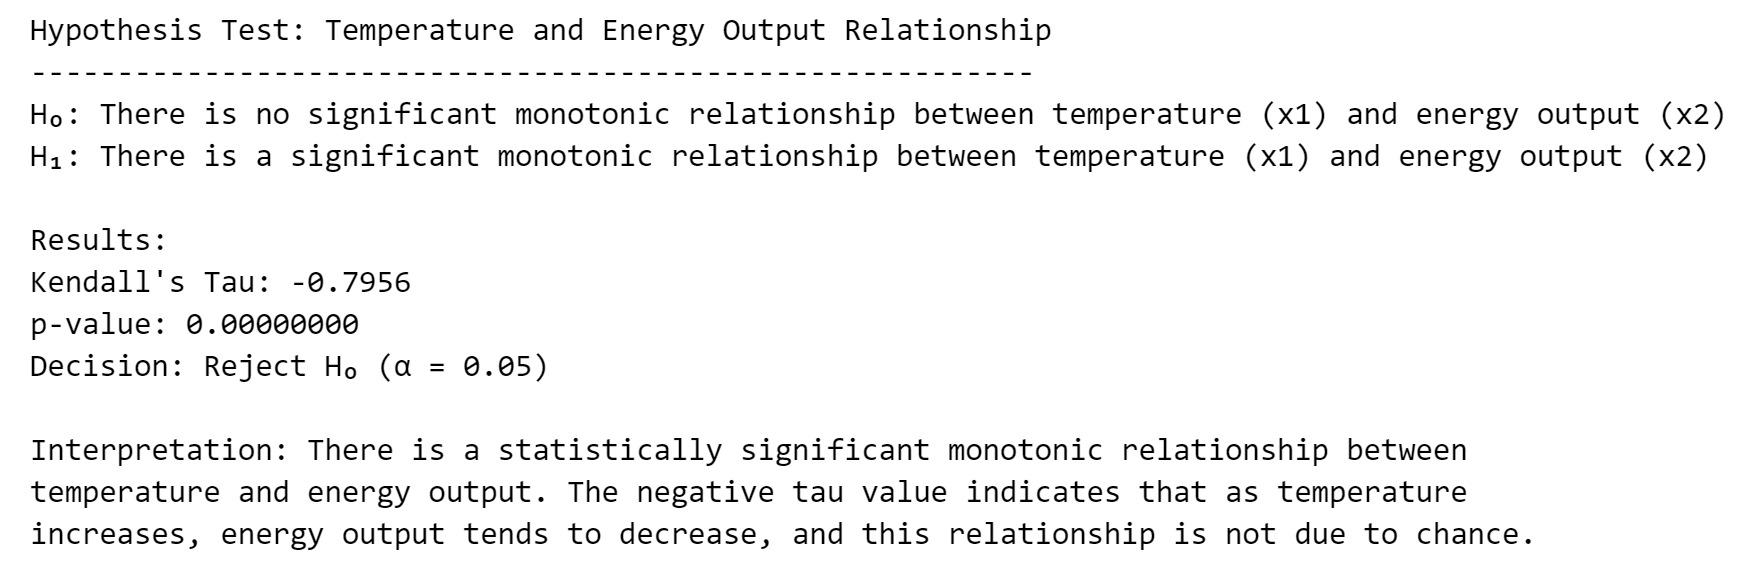
\includegraphics[width=\textwidth]{z13.png}
  %\caption{Hypothesis Test: Relationship Between Temprature and Energy Output}
  %\label{fig:Hypothesis Testing-1}
\end{figure}


Also another test for the multicollinearity between pressure ($x_3$) and vaccum ($x_4$) was conducted using VIF and 
the result obtained is shown below: 

\begin{figure}[H]
  \centering
  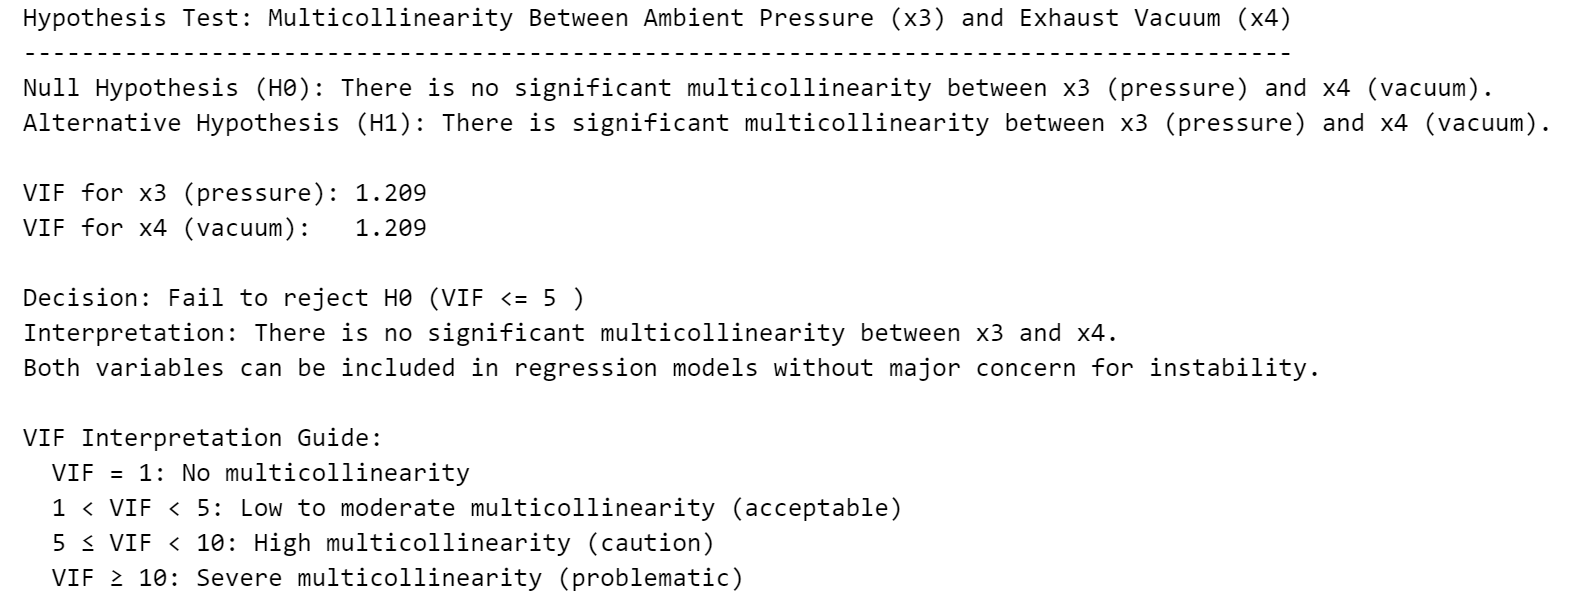
\includegraphics[width=\textwidth]{z14.png}
  %\caption{Hypothesis Test: Multicollinearity Between pressure ($x_3$) and vacuum ($x_4$)}
  %\label{fig:Hypothesis Testing-2}
\end{figure}

And, another test using VIF for multicolinearity between temprature ($x1$) and pressure ($x3$) was 
conducted and the result is shown below: 

\begin{figure}[H]
  \centering
  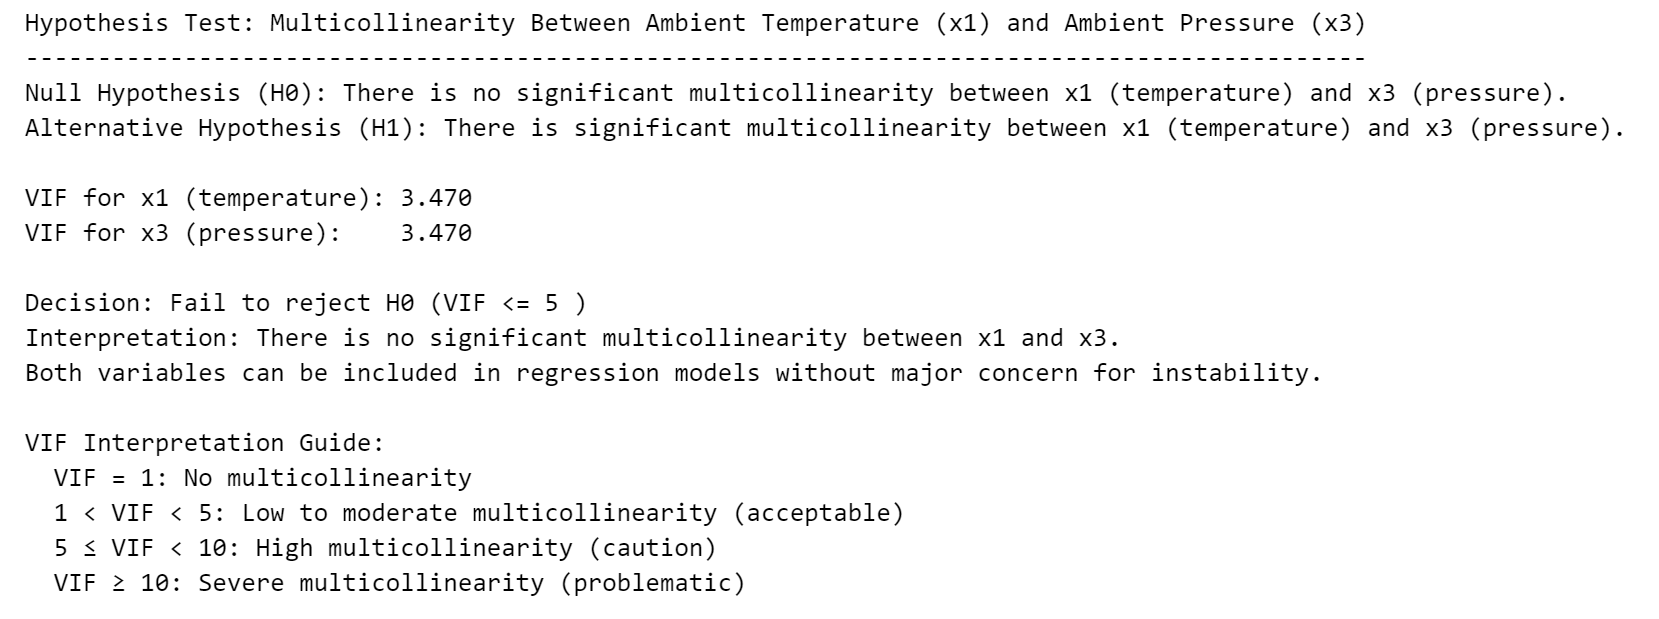
\includegraphics[width=\textwidth]{z15.png}
  %\caption{Hypothesis Test: Multicollinearity between temperature ($x1$) and pressure ($x3$)}
  %\label{fig:Hypothesis Testing-3}
\end{figure}


%-------Model Development and Evaluation-------

\section*{Task 2: Model Development and Evaluation}

%Before modeling, we have conducted a sereis of tests regarding 
%which data transformation is best suitable
%for our dataset, and found Log-Transformation 
%to be a better performing approach in almost all aspects of 
%performance metrics. All the test conducted for such tests 
%can be found in the Github repository in $tests$ section.

%We first prepared the data by Log-Transforming the variables.
%In this transformation we replace each value $x$ in data with $log(x)$ 
%(usually natural log $ln(x)$ or base-10 $log10(x)$). It compresses 
%large values and expands small values, helping reduce data skewness. 
%It turns multiplicative relationships into additive ones, which is 
%often easier for models to handle. Log transformation is only applied 
%to positive numbers (because log of 0 or negative values is undefined).

%The formula for Log-Transformation is:

%\begin{equation}
%  x_{\text{transformed}} = \log(x) + (\varepsilon = -1 \times 10^{-6})
%  \end{equation}  

%Here, $x$ is the original value, $log(x)$ is the natural logarithm with base $e$.

%We also added a small constant $\varepsilon = -1 \times 10^{-6}$ to avoid $log(0)$; as if data contains zeros or negatives then 
%$log(0)$ is not defined.

The following models were evaluated and estimated the parameters for: 

%\begin{itemize}
%  \item Model 1: $y = \theta_1 x_4 + \theta_2 x_3^2 + \theta_{\text{bias}}$
%  \item Model 2: $y = \theta_1 x_4 + \theta_2 x_3^2 + \theta_3 x_5 + \theta_{\text{bias}}$
%  \item Model 3: $y = \theta_1 x_3 + \theta_2 x_4 + \theta_3 x_5^3$
%  \item Model 4: $y = \theta_1 x_4 + \theta_2 x_3^2 + \theta_3 x_5^3 + \theta_{\text{bias}}$
%  \item Model 5: $y = \theta_1 x_4 + \theta_2 x_1^2 + \theta_3 x_3^2 + \theta_{\text{bias}}$
%\end{itemize}


\begin{figure}[H]
  \centering
  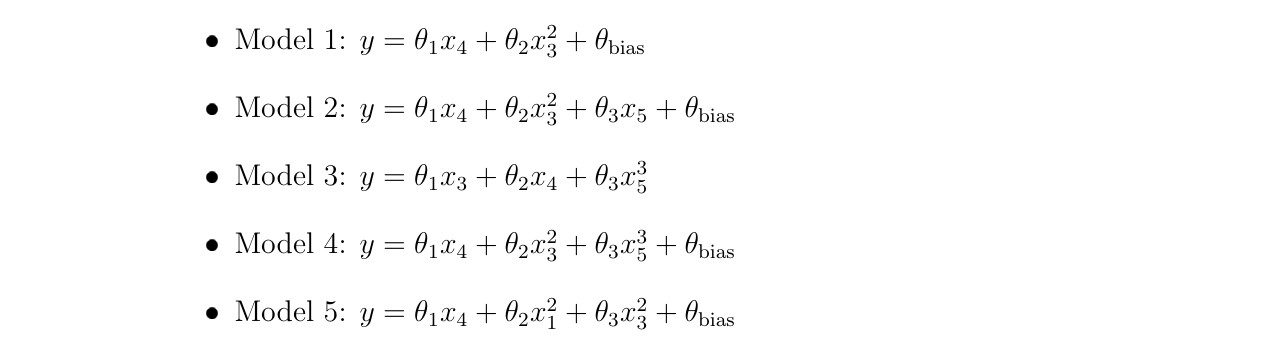
\includegraphics[width=\textwidth]{p1.png}
  %\caption{Given 5 models}
  %\label{fig:Models}
\end{figure}

%----------------Task 2.1-----------------------

\subsection*{Task 2.1: Parameters Estimation}

To find optimal model parameters, we were requested to use a direct relation called normal 
equation. This method helps to calculate optimal model parameters without running loops or
without using trial-and-error methods. We organize essential input data into a metrix form called 
"design metrix". In design matrix, each row represents one observation or one data point. Each column 
represents a feature including a column of 1's for intercept or bias. %Working with this 
%matrix-form helps us to make calculations fast and more efficient and it's god's blessing when 
%dealing with huge data.

%In R, functions were created to construct Design Matrix for different 
%models. Following is R-code to create design matrix for model 1 (for example):

%\begin{figure}[H]
%  \centering
%  \includegraphics[width=\textwidth]{plot203.png}
%  \caption{Create Design Matrix for Model 1: ($y = \theta_1 x_4 + \theta_2 x_3^2 + \theta_{\text{bias}}$)}
%  \label{fig:design_matrix_model_1}
%\end{figure}

%The output "\( \text{model\_1\_matrix} \)" is the design matrix for 
%model-1, which was then used to compute optimal model parameters for model 1
%using Ordinary Leaste Squares (OLS).

The mathemetical expression for Ordinary Least Squares is: 

%\begin{equation}
%\boldsymbol{\theta} = (\mathbf{X}^T \mathbf{X})^{-1} \mathbf{X}^T \mathbf{y}
%\end{equation}

\begin{figure}[H]
  \centering
  
\includegraphics[width=\textwidth]{p2.png}
  %\caption{Given 5 models}
  %\label{fig:Models}
\end{figure}

Where, $\boldsymbol{\theta}$ is the vector of estimated model parameters, $\mathbf{X}$ is 
the design matrix containing the input features or independent variables, and
$\mathbf{y}$ is the vector of observed target values.

In R, a function \(\text{estimate\_parameters()}\) was defined to 
apply OLS, where operations like matrix multiplications, 
matrix transpose and matrix inverions were performed. The \( \text{solve()} \) 
method was used to perform inverse matrix operations.

%\begin{figure}[H]
%  \centering
%  \includegraphics[width=\textwidth]{plot204.png}
%  \caption{Impliment Ordinary Least Squares (OLS) Estimation}
%  \label{fig:Ordinary Least Squares (OLS) Estimation}
%\end{figure}

\texttt{estimate\_parameters()} was called for each model using 
their respective design matrix to estimate the model parameters. 
The \texttt{estimate\_parameters()} function actually performs the model training 
behind the scenes and finds the optimal model parameters for each model.
The calculated model parameters are listed in a tabular structure
for easy reference: 

\begin{figure}[H]
  \centering
  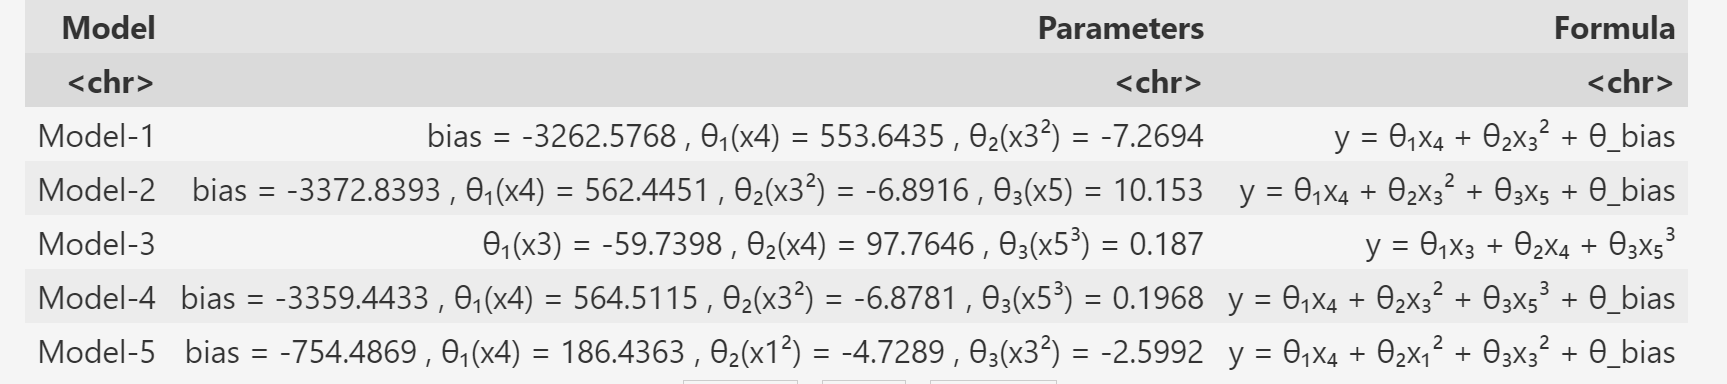
\includegraphics[width=\textwidth]{y1.png}
  \caption{(Optimed Model Parameters Calculated Using OLS)}
  \label{fig:Optimized Model Parameters}
\end{figure}

The estimated optimum model parameters fits into the model equation as follows (used model-1 
as an example): 

\begin{figure}[H]
  \centering
  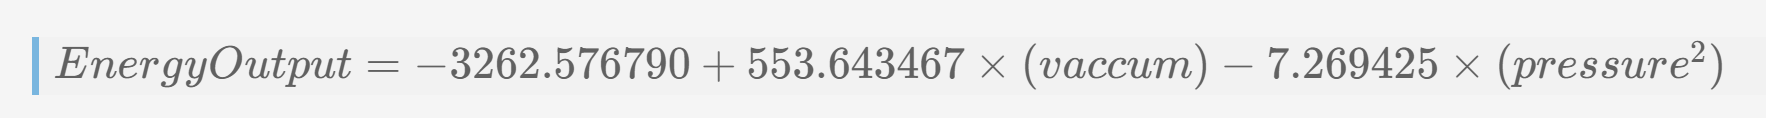
\includegraphics[width=\textwidth]{y2.png}
  %\caption{}
  %\label{fig:}
\end{figure}

The $bias$ $(-3262.576790)$ is the intercept term and it represents the baseline energy output 
when all other variables are zero. Theoretically this is the energy 
output when all other parameters set to constant or zero. But, 
practically, this will never happen because $Exhaust$ $vacuum$ $(cmHg)$: $always  > 0$ 
(total vacuum is impossible) and; 
$Pressure$ $(millibars)$: $always > 0$ (vacuum would imply system failure).

The coefficient for relative humidity ($x4= 8.79$) indicates
assuming all other variables constant, for 1 unit 
increase in humidity results in $8.79$ units
increase in energy.

The coefficient for square of pressure ie. $x_3^2$ = $-0.35$
means as the square of pressure increases, the 
energy output decreases. This is a 
non-linear relationship. 

%----------------Task 2.2-----------------------

\subsection*{Task 2.2: Residual Sum of Squares (RSS)}

In regression, a residual is the difference between the model prediction and give actual value.
This difference tells us how far our model prediction is
for each point. The residual for $j-th$th point is calculated as: 

\begin{figure}[H]
  \centering
  
\includegraphics[width=\textwidth]{p4.png}
  %\caption{}
  %\label{fig:}
\end{figure}

Where; ($y_j$) is the actual value for $j-th$ point and, ( $\hat{y}_j $\) 
is the predicted value for $j-th$ point. 

We take the sum of the squares of all the residuals to measure the overall error in the prediction.  
A smaller value means the predictions closer to actual values.

%\begin{equation}
%RSS = \sum_{j=1}^{n} (y_j - \hat{y}_j)^2
%\end{equation}

\begin{figure}[H]
  \centering
  
\includegraphics[width=\textwidth]{p3.png}
  %\caption{}
  %\label{fig:}
\end{figure}

Here, residuals are squared so they do not cancel out each other, and to give more weight to 
larger errors.

%In R, Residual Sum of Squares can be claculated using following function: 

\begin{figure}[H]
  \centering
  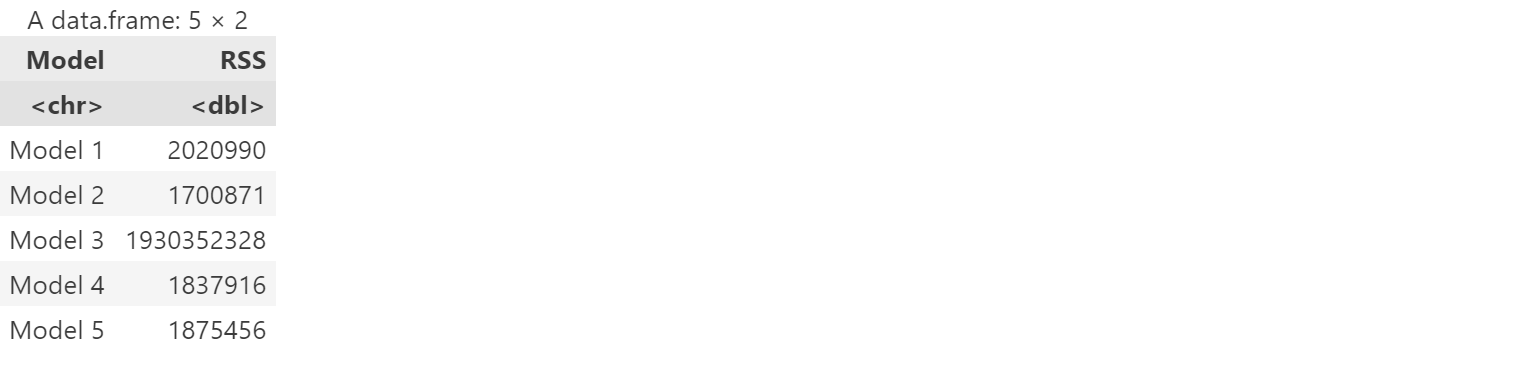
\includegraphics[width=\textwidth]{m1.png}
  %\caption{(RSS-Values)}
  %\label{fig:Calculate RSS}
\end{figure}

Smaller residual sum of squares means the model is making small errors. Here from above comparision table, model 
5 has the smallest RSS value ($RSS= 198462.5$) followed by model 4 ($RSS= 515095.0$) and model 2
($RSS= 516315.9$). Model 3 ($RSS= 568957.4$) has the higest value among all the given models.
Considering RSS values, model 5 is performing well while model 3 is lagging well behind possibly due to 
the abscence of bias term. 

%----------------Task 2.3-----------------------

\subsection*{Task 2.3: Log-Likelihood}

%In regression, log-likelihood is used to 
%ananyze the model performance. In general, 
Log-Likelihood tells- 
how good is the model at explaining the 
data we have observed. It assumes the residuals are 
normally distributed. 
LL measures the closeness of predicted values to  
the actual values by taking into account how spread 
out the residuals are (the variance). 

The mathemetical expression to calculate log-likelihood is: 

%\[
%\log L = -\frac{n}{2} \log(2\pi\sigma^2) - \frac{1}{2\sigma^2} \sum_{i=1}^{n} (y_i - \hat{y}_i)^2
%\]

\begin{figure}[H]
  \centering
  
\includegraphics[width=\textwidth]{p5.png}
  %\caption{}
  %\label{fig:}
\end{figure}

Where: $n$ = number of observations, $\sigma^2 $ = variance of residuals,  
$y_i$ = actual value,  $\hat{y}$ = predicted value. 

%In R, a custom function was used to calculate
%log-likelihood for each model:

\begin{figure}[H]
  \centering
  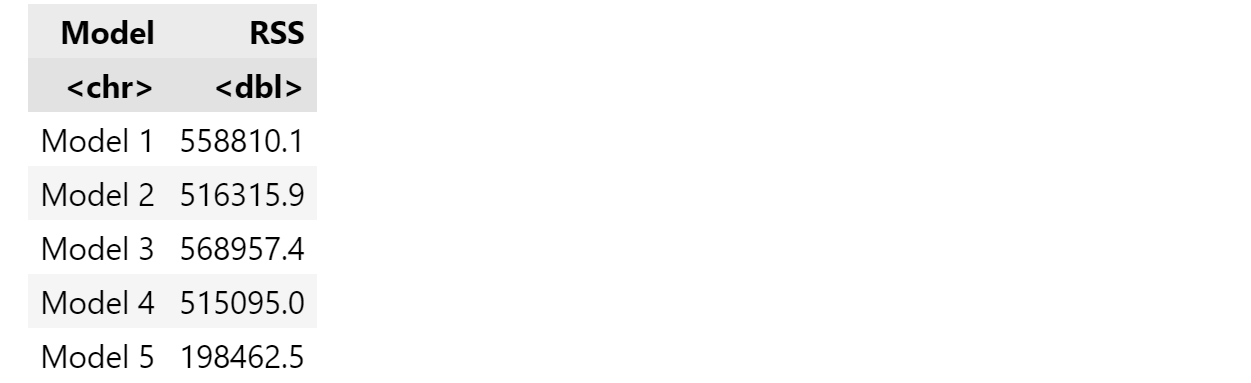
\includegraphics[width=\textwidth]{m5.png}
  %\caption{(LL- values for different models)}
  %\label{fig:Log-Likelihood}
\end{figure}

High log-likelihood value means the model fits the data better. Model 5 has comperatively largest  
value of ($LL= -27982.45$) followed by model 4	($-32525.65$). The model 3 has shows smallest
log-likelihood value ($-32999.4$). Based on the LL-values, model 5 is again performing well. And, 
model 3 is not of the great choice again possible because this model is 
not capturing the underlying relation between the environmental variables 
and the output.  

%Log-likelihood is also an important part for 
%some other important model selection methods like
%Akaike Information Criterian (AIC) and Bayesian 
%Information Criteian (BIC) which we use next. 
%----------------Task 2.4-----------------------

\subsection*{Task 2.4: AIC and BIC}

AIC is a numerical value that helps us decide which 
model fits the data best. It takes into consideration 
two things: how well the model fits the data and 
how simple the model is. BIC and AICs are similar concepts but they differ in one thing; BIC gives more penalty 
for complex models and prefers simpler models even more. %This tries to avoid overfitting 
%by penalizing models that use too much variables. Interpretation is
%simple: low AIC is better.

Interpretation is similar: low is better. 
Both are used to compare different models; and 
they are not to judge single model alone.

The formulas to calculate these Valuesare as follows:


\begin{figure}[H]
  \centering
  
\includegraphics[width=\textwidth]{p6.png}
  %\caption{}
  %\label{fig:}
\end{figure}

%\begin{equation}
%\text{AIC} = 2k - 2\log L
%\end{equation}
%\begin{equation}
%\text{BIC} = k \log n - 2\log L
%\end{equation}

where, $k$: number of model parameters, $n$: number of observations, and 
$\log L$: log-likelihood calculated earlier. 

%In R, a function to calculate AIC and BIC can be written as follows:

%\begin{figure}[H]
%  \centering
%  \includegraphics[width=\textwidth]{plot23_aicbic.png}
%  \caption{(Function to calculate AIC, BIC in R)}
%  \label{fig:Calculate AIC and BIC}
%\end{figure}

%The following table gives the summary of all 
%the important model evaluation statistics we have calculated until now. 
%This includes the residual sum of squares (RSS), 
%log-likelihood, AIC, BIC, and other relevant statistics:

\begin{figure}[H]
  \centering
  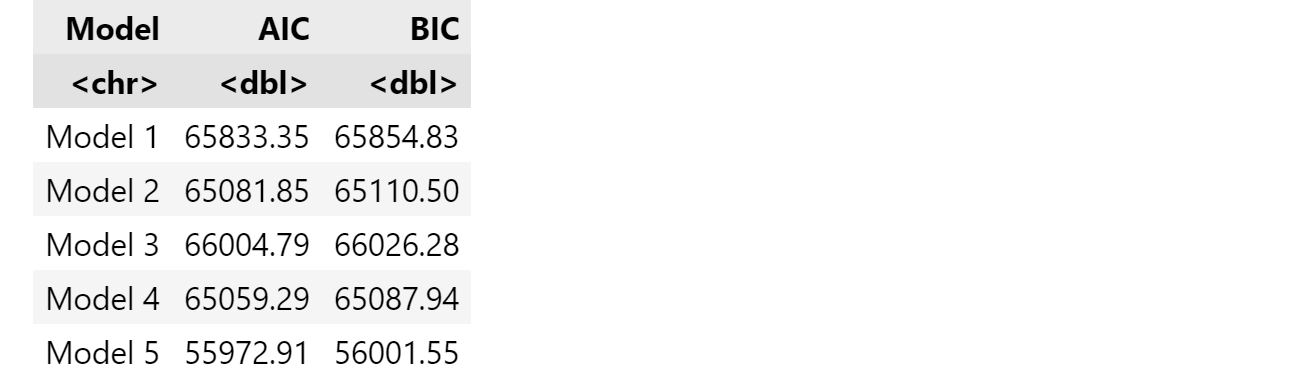
\includegraphics[width=\textwidth]{m6.png}
  %\caption{(Comparision: AIC and BIC values)}
  %\label{fig:Comparision Table AIC and BIC}
\end{figure}

Model 5 is clearly better with $AIC= 55972.91$ and $BIC=	56001.55$. Model 4 
is just behind model 5 with $AIC= 65059.29$	and $BIC= 65087.94$. Model 3 is still 
lagging and reserves the fifth position with $AIC= 66004.79$	and $BIC= 66026.28$. 
All the performance metrices indicates model 5 is performing 
comparatively well whereas model 3 is performing poorly. 

%----------------Task 2.5-----------------------

\subsection*{Task 2.5: R-squared($R^2$), Adjusted R-squared ($R^2_{\text{adj}}$), Root mean squared error ($RMSE$) and Mean percentage error ($MPE$)}

Some other regression metrics like R-squared($R^2$), adjusted R-squared ($R^2_{\text{adj}}$), 
root mean squared error ($RMSE$) and mean percentage error ($MPE$) were also calculate to support the 
regression metrics we have calculated above ($RSS$, $LL$, $AIC$ and $BIC$). Detailed explaination 
along with how to calculate each metric is given in the appendix.

%R-function for calculating there metrics were defined and applied to 
%estimate the corresponding metrics for all the models. 

Below table represents a summary of the statistics that we have calculated which acts as 
the additional performance comparision metrics: 

\begin{figure}[H]
  \centering
  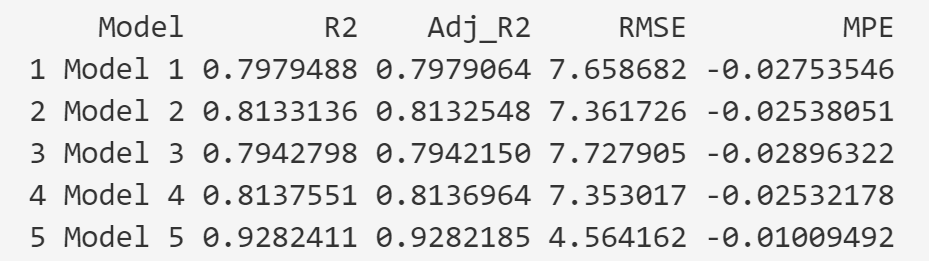
\includegraphics[width=\textwidth]{y5.png}
  \caption{(R-Squared, Ajusted R-Squared, RMSE, MPE)}
  \label{fig:Comparision Table}
\end{figure}

Model 5 again is better-performing model, 
with the highest R-squared ($= 0.9282$) and adjusted R-squared ($=0.9282$), indicating it explains the largest 
proportion of variance in the target variable. 
It also has the lowest RMSE ($=4.5642$) and smallest MPE ($=-0.0101$), 
meaning it's the most accurate and least biased in predictions.

Model 3 is again the worst-performing model, with the lowest R-squared ($=0.7943$), 
lowest adjusted R-squared ($=0.7942$), highest RMSE ($=7.7279$), and most negative MPE ($=-0.0290$). 
This indicates that it explains the least variance, makes the largest errors, 
and has the greatest bias among all models. Model 3 is likely missing important 
nonlinear terms or interactions that other models (especially Model 5) capture.

%------------Task 2.6----------------------------------
\subsection*{Task 2.6: Distribution of Residuals}

%Residuals are the differences between actual and 
%predicted values from a regression model. They
%show the accuracy of the predictions and helps to
%check if the model is working well or not. 

%Small and randomly scattered residuals indicates
%a good model fit. 
In regression, the
residuals should be normally distributed with 
zero mean and a constant spread or variance 
across all values, this phenomenon is called 
homoscedasticity. If the residuals shows some
pattern then it generally indicates that the model 
is missing something like missing important 
variables, very complex relationship between 
variable which is not being captured by the current
modeling approach or the situation where 
predictor variables are highly correlated with each
other.

We calculated some basic statistics on residuals
like mean, median, standard devition, skewness etc. and
their summary is presented in the table below: 

\begin{figure}[H]
  \centering
  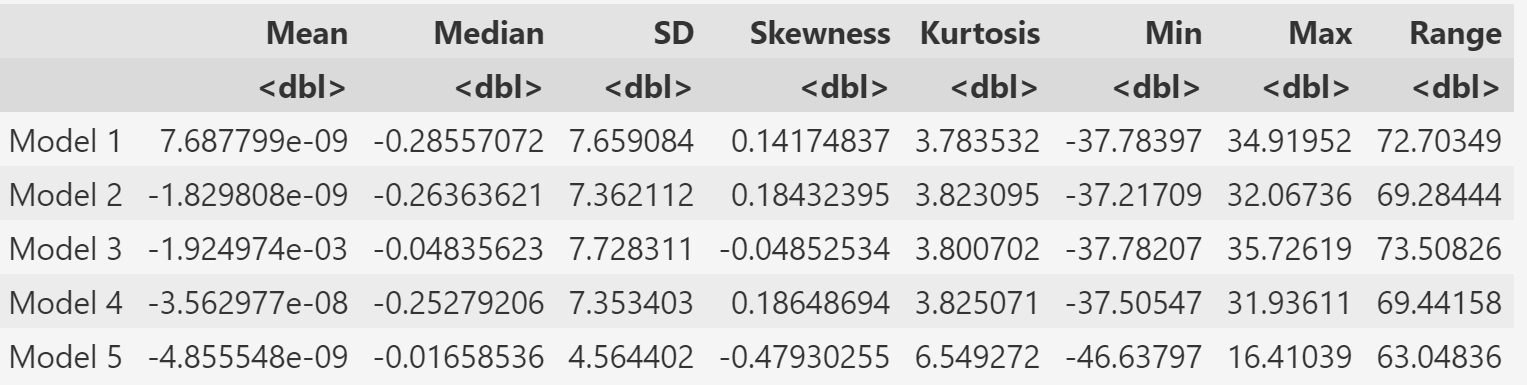
\includegraphics[width=\textwidth]{y6.png}
  \caption{(Residual Statistics Comparision Table)}
  \label{fig:Comparision Table}
\end{figure}

To get an idea of how the the residuals are distributed,  
histogram along with density and rug plots were constructed and present in the 
following plot: 

\begin{figure}[H]
  \centering
  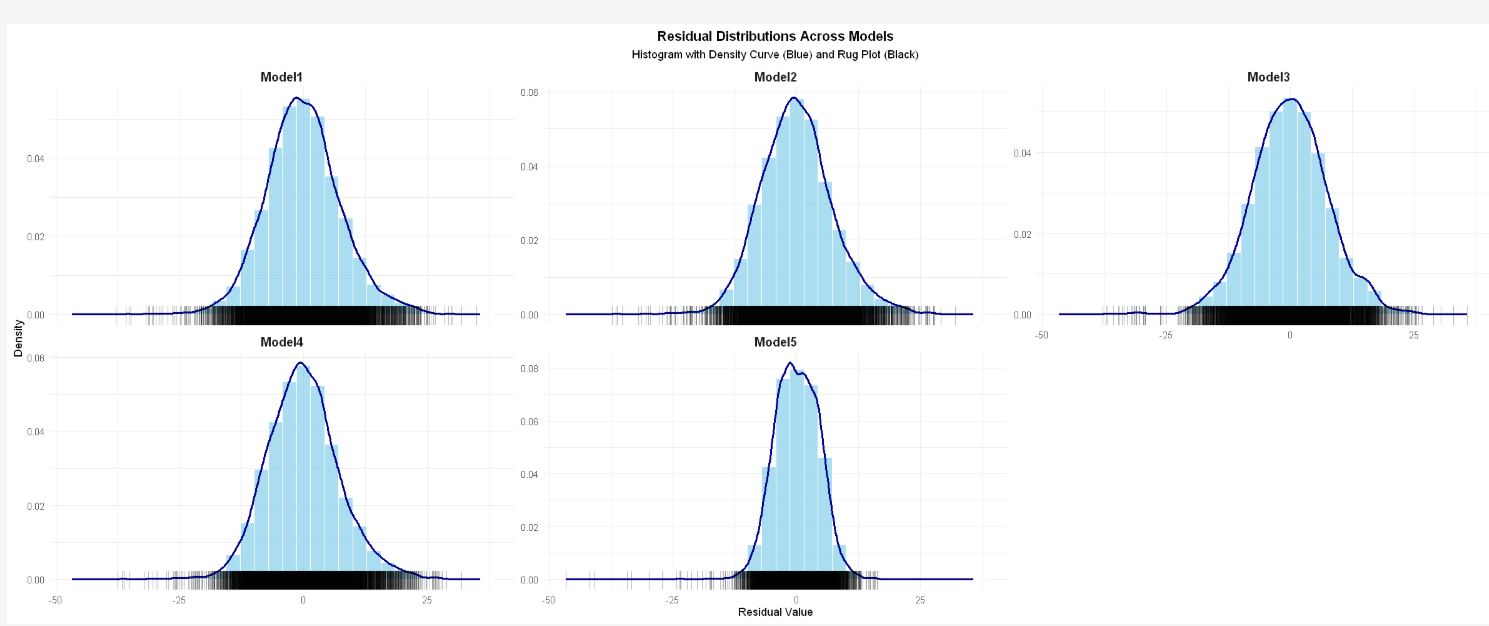
\includegraphics[width=\textwidth]{y8.png}
  \caption{(Residual Statistics Comparision Table)}
  \label{fig:Comparision Table}
\end{figure}

Residuals were standerzed using z-score standerization and QQ-plot for each of the
models were drawn, where, straight diagonal line represents the theoretical quantiles 
and colored points represents the actual quantiles of residuals for each model:

\begin{figure}[H]
  \centering
  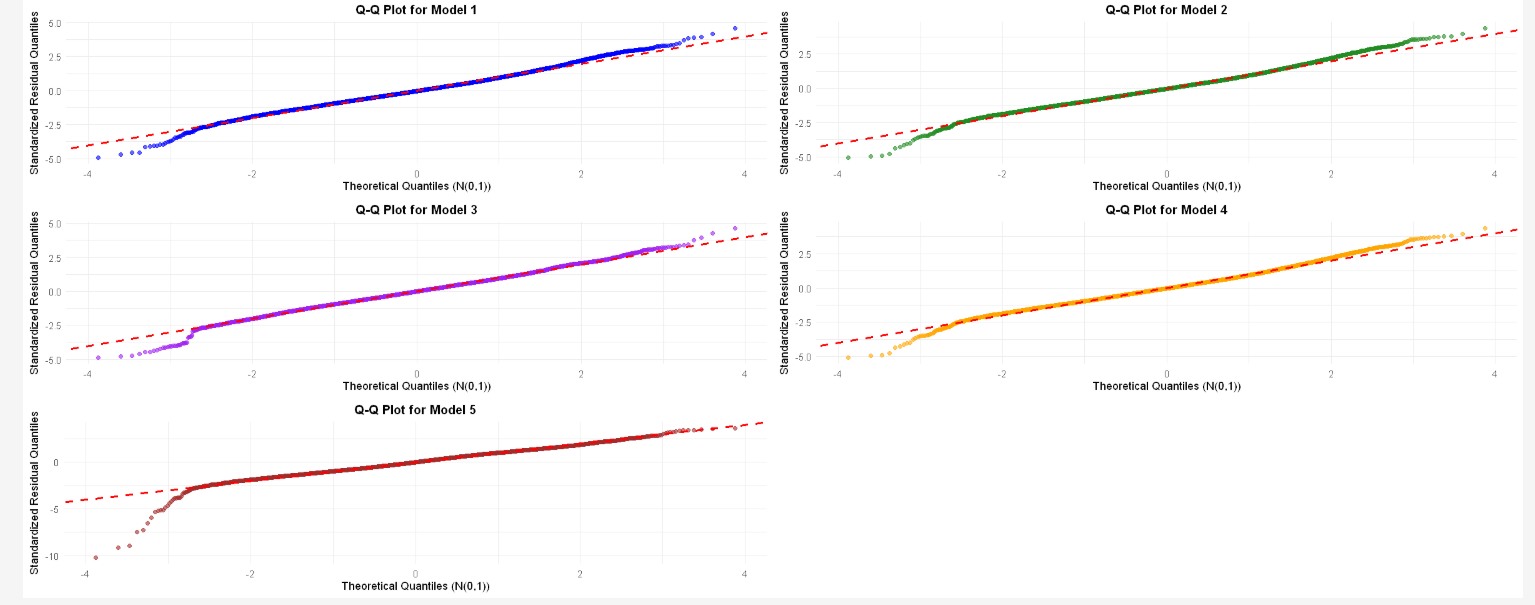
\includegraphics[width=\textwidth]{y9.png}
  \caption{(QQ-Plots of Standerized Residuals)}
  \label{fig:Comparision of Residuals Normality}
\end{figure}

%On each plot, x-axis represents the theoretical quantiles from a standard normal 
%distribution $\mathcal{N}(0, 1)$, and y-axis represents the 
%standardized residual quantiles for each model. 
%The dots represent the observed residual quantiles, and the 
%red dashed line indicates the reference line for perfect normality. 

%In each plot, most points approximately lie
%along the red dashed line, which is an indication that the residuals are roughly 
%normally distributed. However, 
Almost all models show slight deviations at 
the lower left tails, suggesting mild to moderate tails and potential outliers. 
The residuals for model 1 and 2 are closely alligned with reference line with very little deviations
at the tail ends. Models 3 and 4 also have moderate deviations at the ends.
Model 5 has higest deviations at the left-tail end. It is also notable that residuals distribution for 
each model deviates from normality only at left tail, otherwise there is almost a perfect 
normality.

From normality of residuals, model 1 and 2 are performing well whereas model 5 shows the 
higest deviations at the left tail.

\subsubsection*{Residuals vs. Fitted Values Plot}

Residual vs. fitted values curve is a scatter plot 
where predicted values are on the x-axis and 
residuals on the y-axis. Each point on the curve 
represents how far the model prediction is from the actual
value. 

%This is used to check if the regression model is a 
%good fit or not. This plot helps us to verify some key 
%assumptions in regression like: linearity, constant 
%variance and independence of errors. 

If a model is a good fit then; residuals should be 
randomly scattered around zero, there should be no clear 
pattern or shape and, the spread of the residuals 
should be roughly constant across all the fitted 
values. 

%If there is a clear patterns like; a curve-like shape 
%in the residuals- it indicates the model is missing 
%somthing or it is non-linear; fan shape- non-constant variance; 
%outlier or extreme residuals- indicates the individual 
%data points may be affecting the model too much. 

Relationship between residuals and fitted values were throughly studied, 
and the plots are presented below:

\begin{figure}[H]
  \centering
  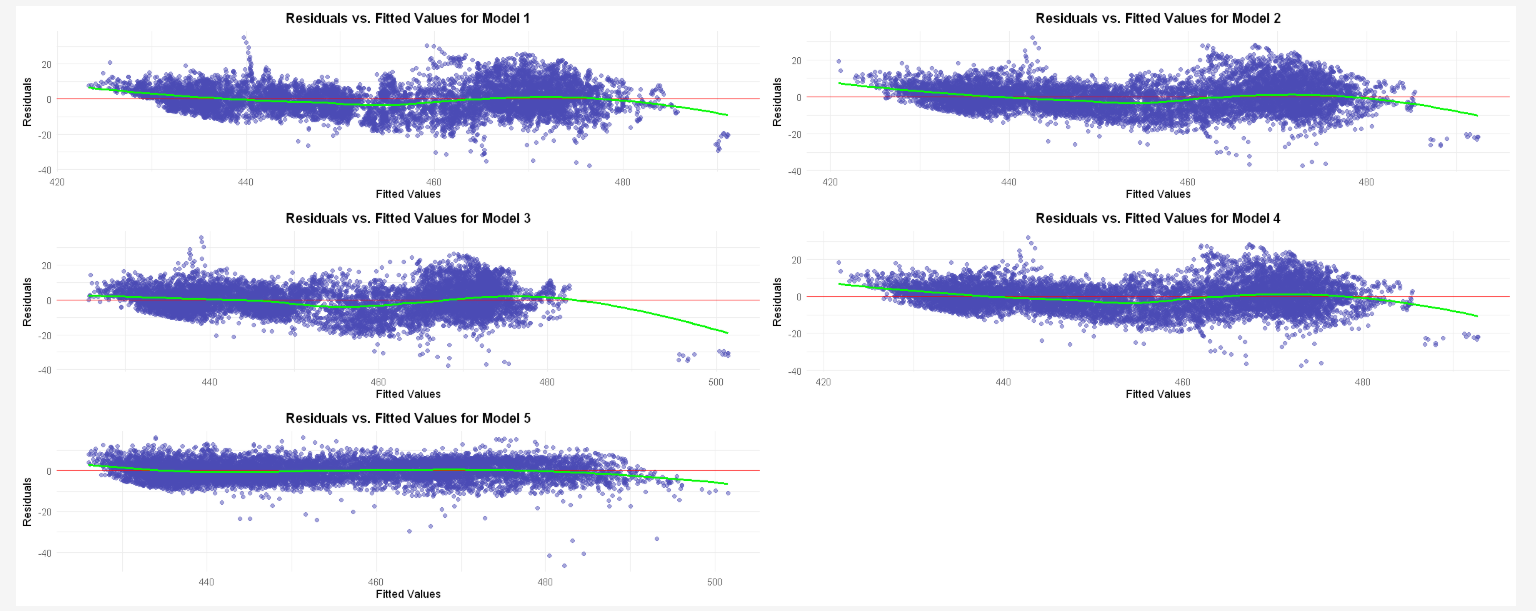
\includegraphics[width=\textwidth]{y10.png}
  \caption{(Comparision: (Residuals vs. Fitted Values))}
  \label{fig:Residuals vs. Fitted Values}
\end{figure}

%The x-axis shows the predicted (fitted) values, and 
%the y-axis shows the residuals 
%(the difference between the actual and predicted values) for each model.

%Residuals are mostly centered 
%around zero, which is good— this means predictions are generally unbiased. 
%Spread of residuals is fairly constant across fitted 
%values (no strong funnel shape), so there’s no major 
%issue with heteroscedasticity (unequal error variance). 
%Slight downward trend in residuals at higher 
%fitted values hints that the models may slightly 
%underpredict at the high end.

For model 5, except some outliers, majority of 
points are grouped arround the reference line 
(red line) with constant variance, no curve or 
funnel shape is seen around the reference line. 
The LOESS (green line) is almost parallel and 
overlapping with the reference (red line); 
indicating model 5 is performing well compared to other models.

By analyzing the residual vs. fitted values curves; 
model 5 emerges out as the better performing model among the given models. 

%----------------Task 2.7-----------------------

\subsection*{Task 2.7: Selecting Better Performing Model}

The following table provides comparison for all 
candidate models. It includes key performance metrics such as $RSS$, $AIC$, 
$BIC$, log-likelihood values ($LL$), residual statistics along with $MSE$, $R-squared$:

\begin{figure}[H]
  \centering
  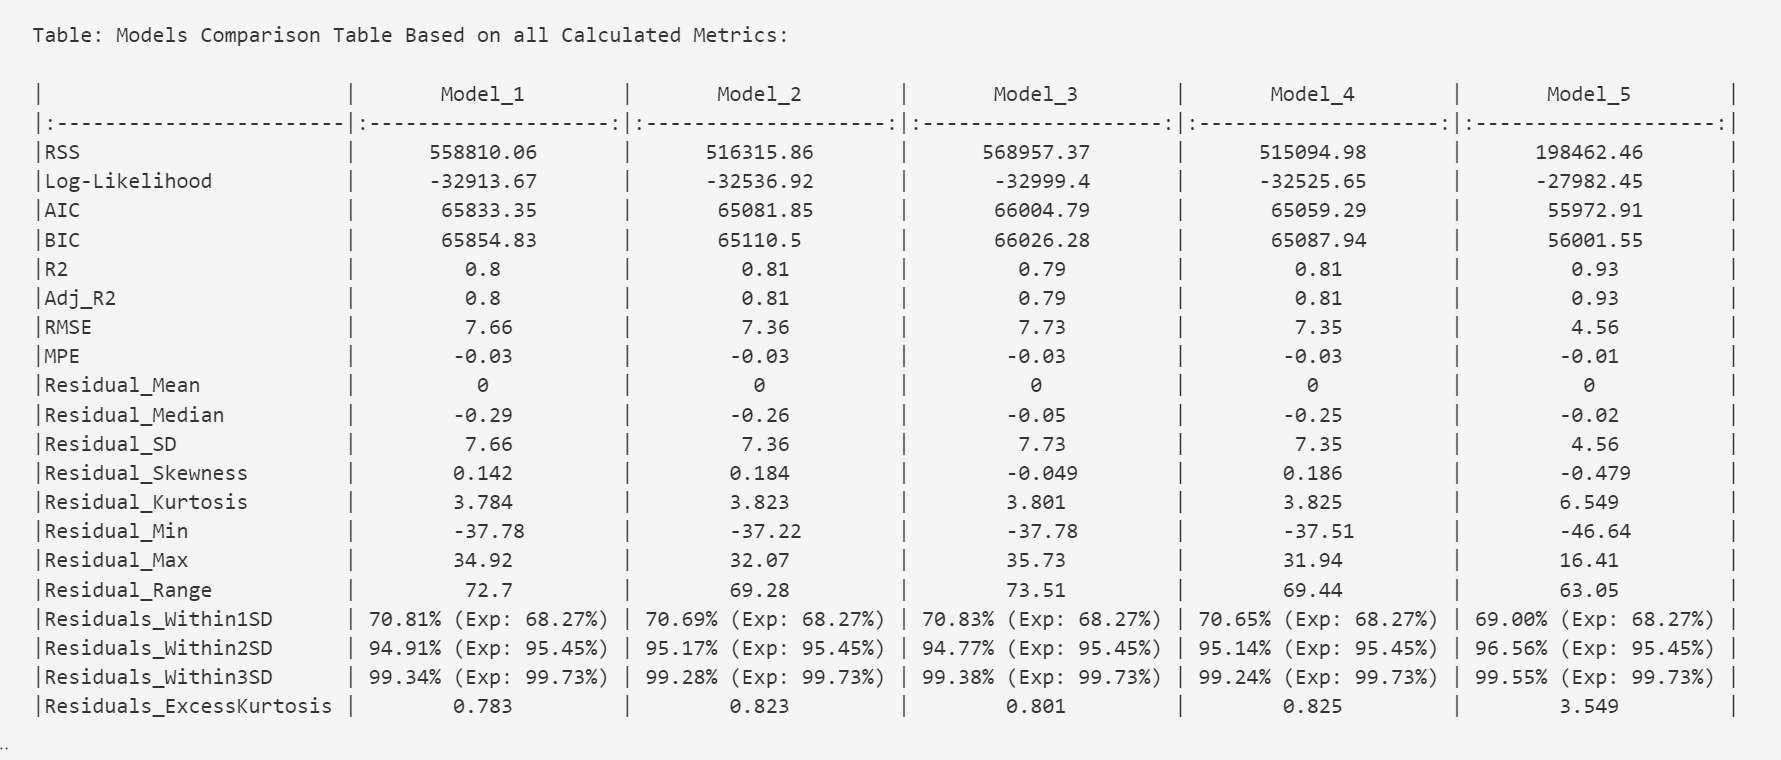
\includegraphics[width=\textwidth]{y12.png}
  \caption{(Comparision of Models based on their performance Statistics)}
  \label{fig:Model Selection}
\end{figure}

%Model 5 is choosen as the better performing model based on 
%the metrics and statistics from the comparision table above.

For model 5, we have the higest AIC ($=55,972.91$) and BIC ($=56,001.55$) values, 
have lowest RSS ($=198,462.46$) value and higest LL value ($=-27,982.45$) among 
all the contestent models. These values indicates a strong 
balance between model fit and simplicity. Model 
5 also have higest adjusted R-squared ($=0.93$) R-squared ($=0.93$) values. 
Model 5 is also best in prediction which have lowest 
RMSE ($=4.56$) and RSD ($=4.56$) which indicates  
very small average errors. MPE is ($= -0.01$) 
which is very close to zero so the model 
has very little bias in predictions. 

QQ-plot for model 5 is also acceptable but is not best among other models, model-1 and model-2 have 
more normal-like curves. Model 5 show deviations from normal look particularly at the lower left tail
but still it is good overall. Plotted histograms and density curves are also acceptably normal which 
otherwise shows mild skewness. 

From residuals vs. fitted values curve; for model 5, except some outliers, 
majority of points are clustered around the reference line (red line) 
with constant variance, no curve or funnel shape of the points around 
the line. 

Based on these evidence - metrics, plots and assumptions; 
model 5 is better performing model among all. It fits the 
data well and, is statistically sound and practically 
useful. 

%----------------Task 2.8-----------------------

\subsection*{Task 2.8: Train-Test Validation}
The data was divided into train and test splits where 70\% of data was used to estimate
the model parameters (for the selected model-2) and remaining 30\% was used to evaluate the model. 

\subsubsection*{Task 2.8.1: Evaluation on Training Data}
The selected model 5 was then trained on training dataset (obtained from the splitting) using OLS method and 
then predictions were made using the estimated parameters. %Then residuals 
%were calculated by taking the difference between predicted and actual values. 
A analysis on the residuals was conducted by plotting histograms with density and rug plots: 
%A histogram, along with a kernel density estimate and 
%rug plot was used to visually assess the distributional 
%characteristics of the residuals: 

\begin{figure}[H]
  \centering
  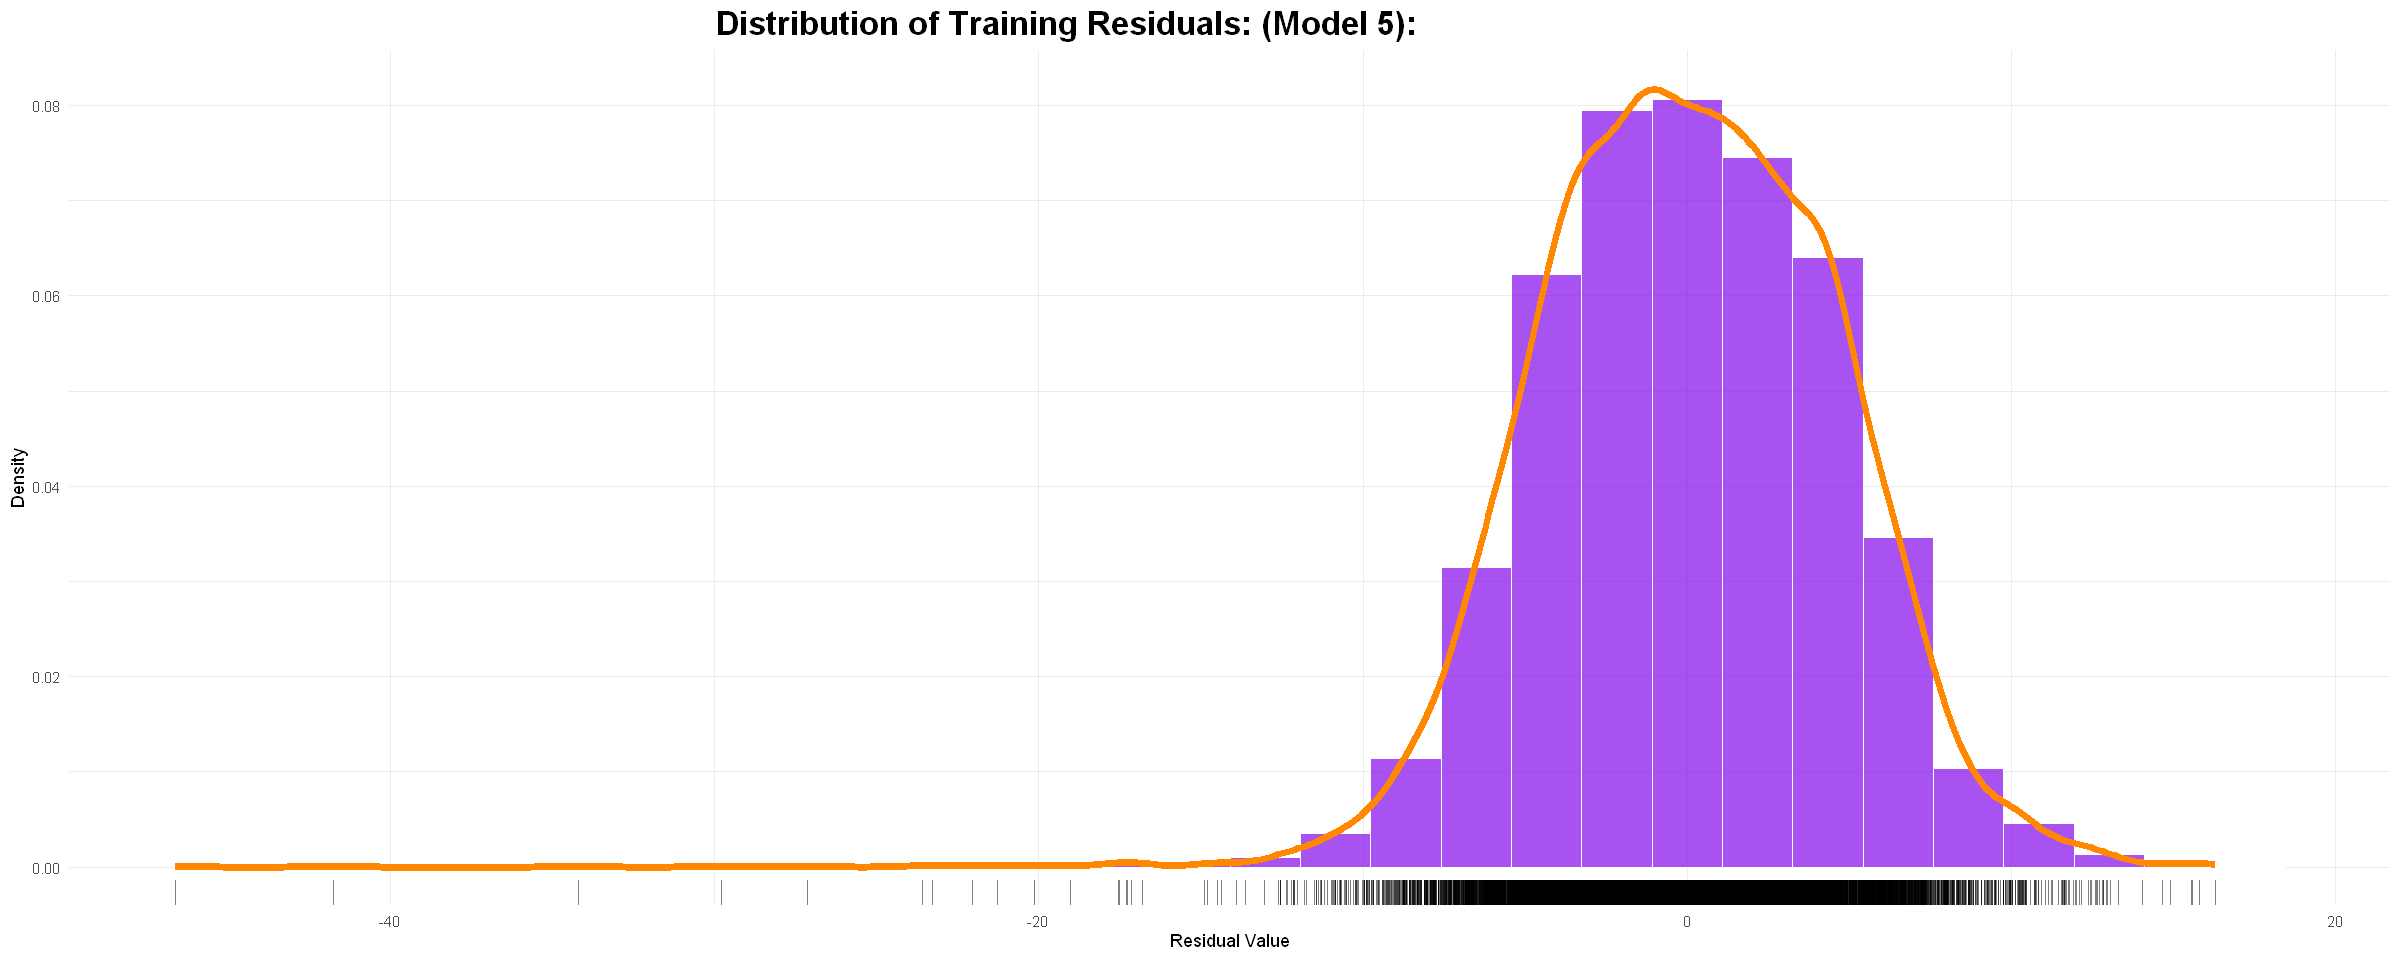
\includegraphics[width=\textwidth]{y16.png}
  \caption{(Distribution of training residuals)}
  \label{fig:Model Selection}
\end{figure}

Due to a few outliers, the distribution appears left-skewed 
but if we omit about 5-6 residuals 
then it is very close to normal distribution.
The residuals form roughly symmetrical (balenced on both sides of zero) curve (omitting few extreme residuals on left side of the curve). 
It has only one peak ( which means it is unimodal), and the plot is almost centered around 
zero ($mean= 0$). The distribution is comparable to the normal distribution. 

%The shape almost resembles the normal 
%distribution. If we remove outliers from the dataset then this will probably become more normal-like.

Scatter plot was created which compares the actual and 
predicted values for the training dataset. 
This get an idea of how well model is performing on the training data. 

%If model is performing well then the predictions and the actual 
%values should be close to each other as possible.

\begin{figure}[H]
  \centering
  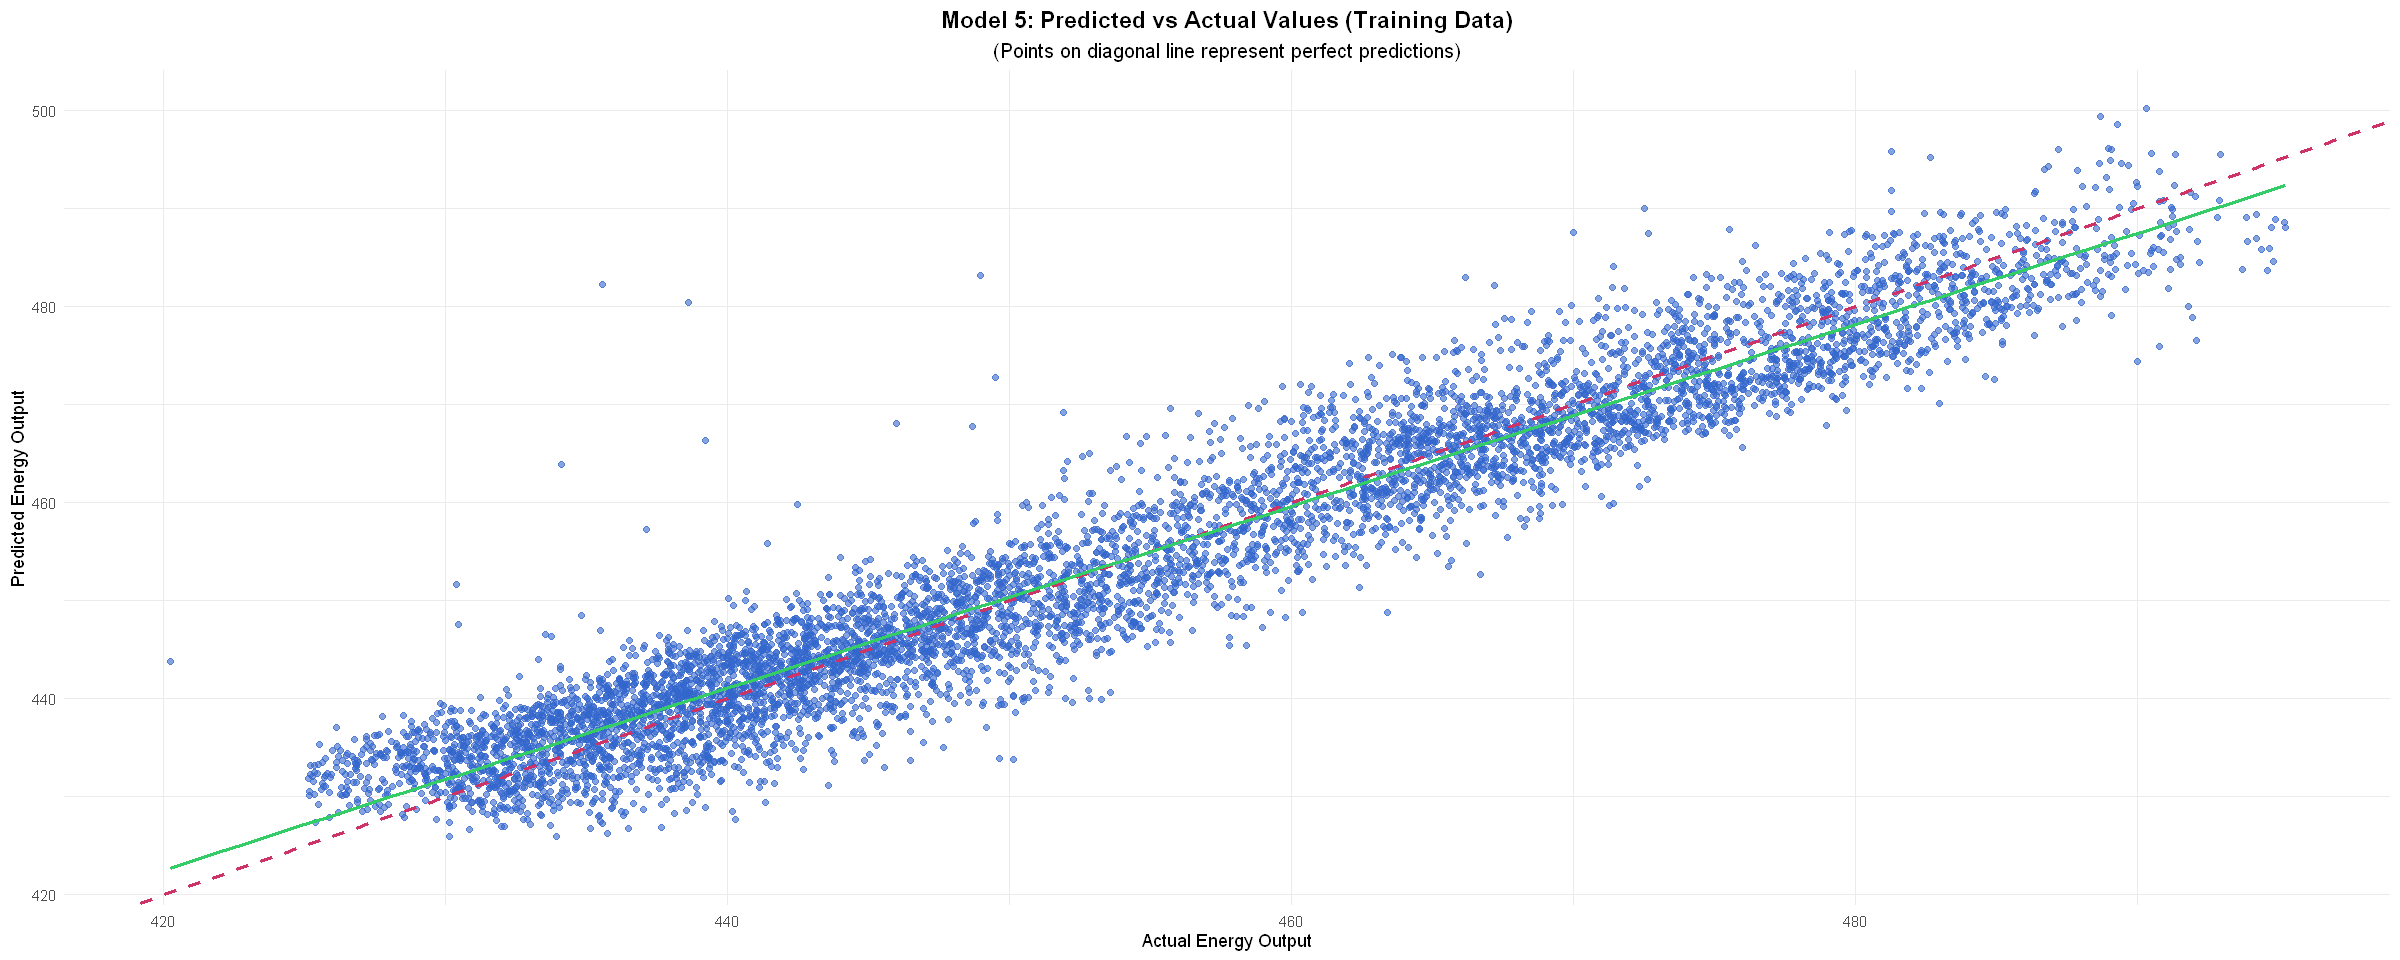
\includegraphics[width=\textwidth]{y17.png}
  \caption{(Scatter Plot: Actual vs. Predicted values)}
  \label{fig:actual vs. predicted values for train dataset}
\end{figure}

%This scatter plot compares model performance by plotting actual values 
%along x-axis and predicted values along y-axis. The red dashed 
%diagonal line ($y = x$) represents perfect predictions, where 
%predicted values match actual values exactly. Points near this 
%line indicate accurate predictions, while those above or below 
%reflect overestimation or underestimation, respectively. 
%A blue trend line is also included to show the general 
%alignment between actual and predicted values, helping to 
%identify any bias or systematic error in the model's output.

Almost all points are clustered around the diagonal line with constant 
variance, which means model’s predictions 
are highly accurate. Very few points are scattered randomly which is normal because it is imposible to
have perfect prediction on each and every observation. The reference line (red) and the overall trend line
are parallel and almost overlap further indicating high prediction accuracy. 

%The points are arranged around the diagonal reference line (red line) 


Next, the 95\% confidence intervals for the predictions were 
computed and plotted alongside actual and predicted values. 
Also, to enhance visualization, a zoomed-in view was generated by 
displaying the first 100 observations: 

\begin{figure}[H]
  \centering
  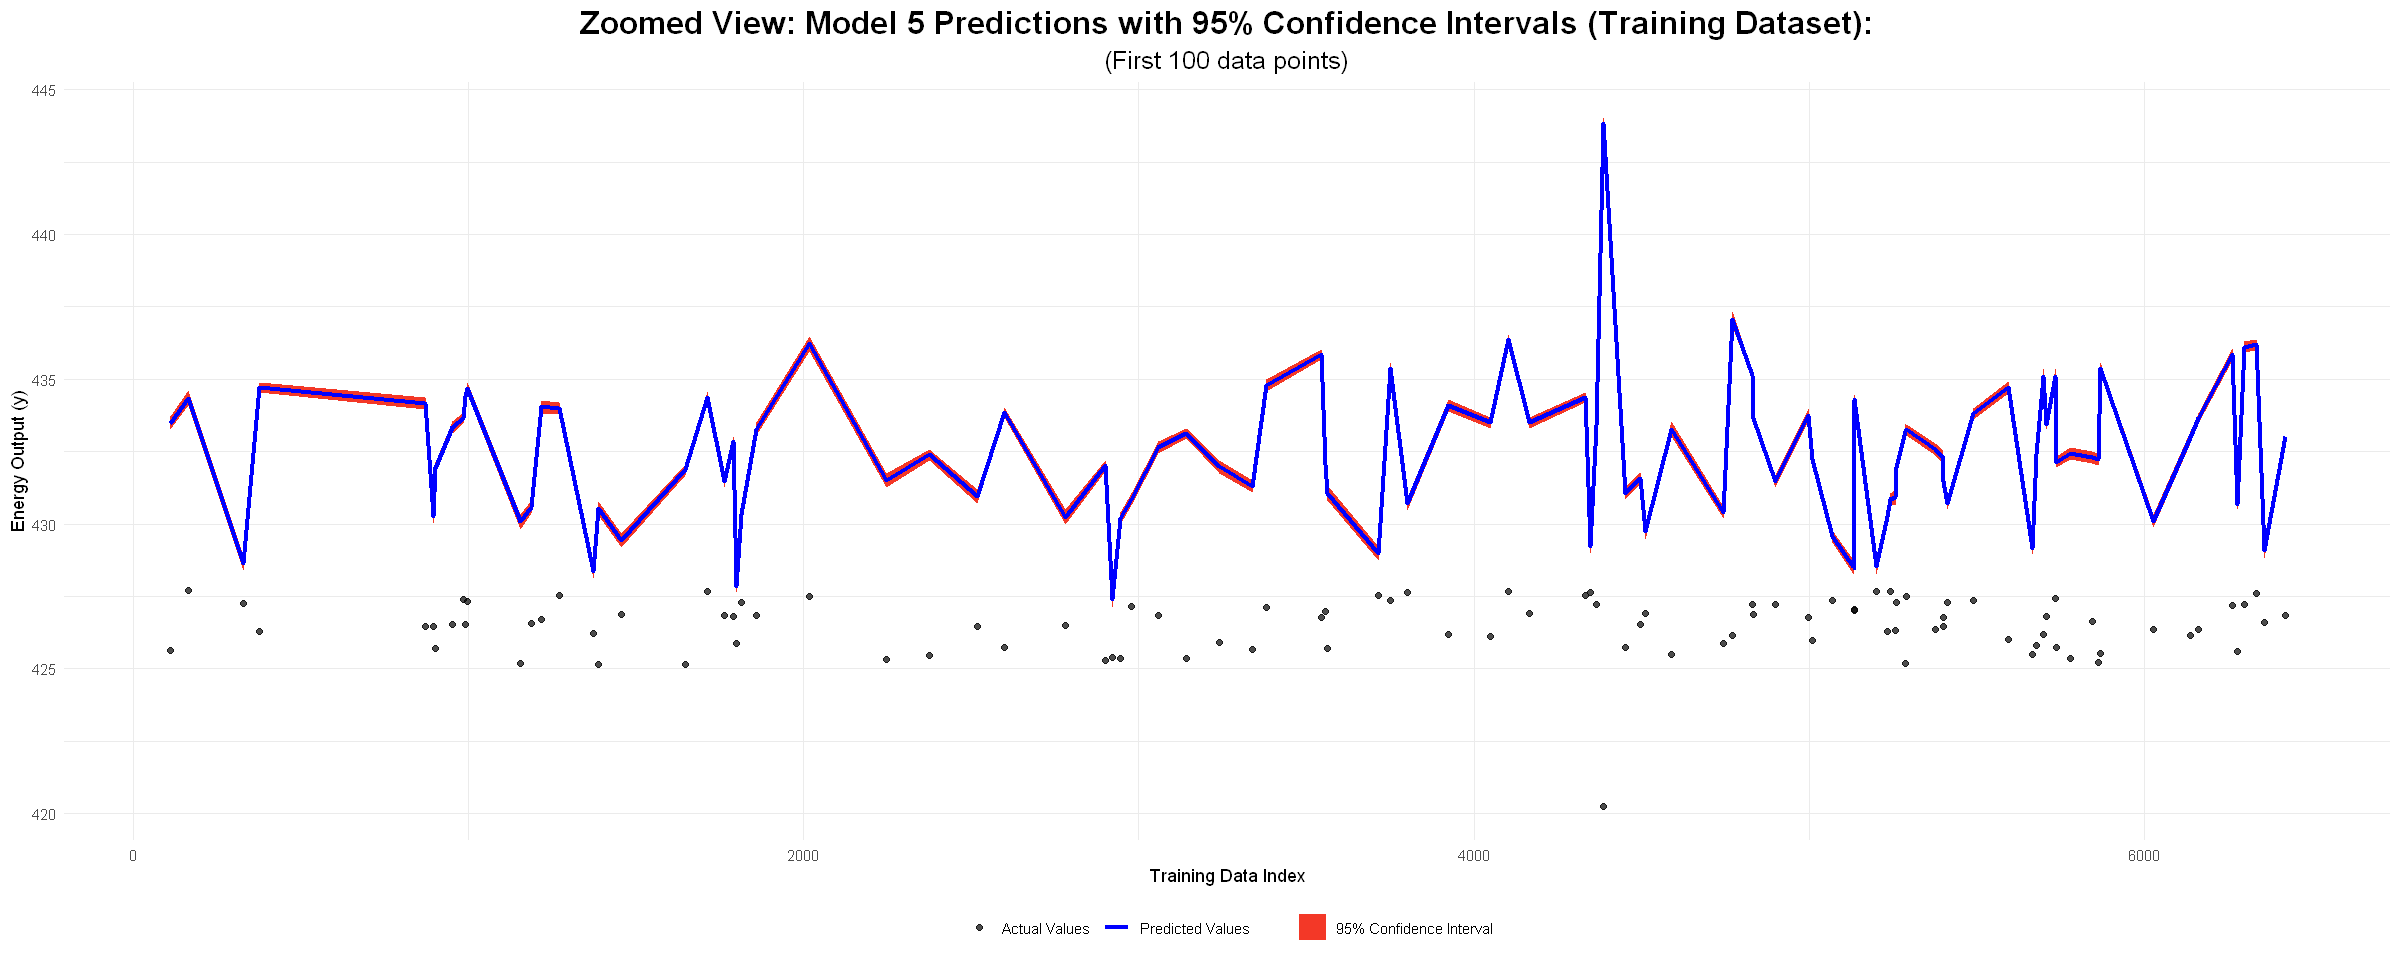
\includegraphics[width=\textwidth]{y18.png}
  \caption{(Model-5 predictions with 95\% Confidence Intervals)}
  \label{fig:Confidence Intervals}
\end{figure}

%This figure presents a zoomed-in view of Model ’s predictions 
%on the first 100 training observations, along with their 95\% confidence 
%intervals. 
The blue line shows the predicted energy output, the red 
ribbon indicates the 95\% confidence interval, and the black 
dots represent the observed values. Most of the black 
dots fall below the blue line, so the model 
slightly over predicts the energy outputs. 
But, since this segment is a small portion of the larger  
training dataset, such over-predictions can be ignored.

Even when zoomed in, the confidence intervals remain very narrow, 
indicating low uncertainty in the predictions. This
suggests the model performs well on the training data.

For the 95\% confidence intervals, error bars were plotted 
and expanded by a factor of 10 to make them visible on the plot. 
These enlarged intervals were intended solely for better visualization 
and do not represent the true statistical width.

\begin{figure}[H]
  \centering
  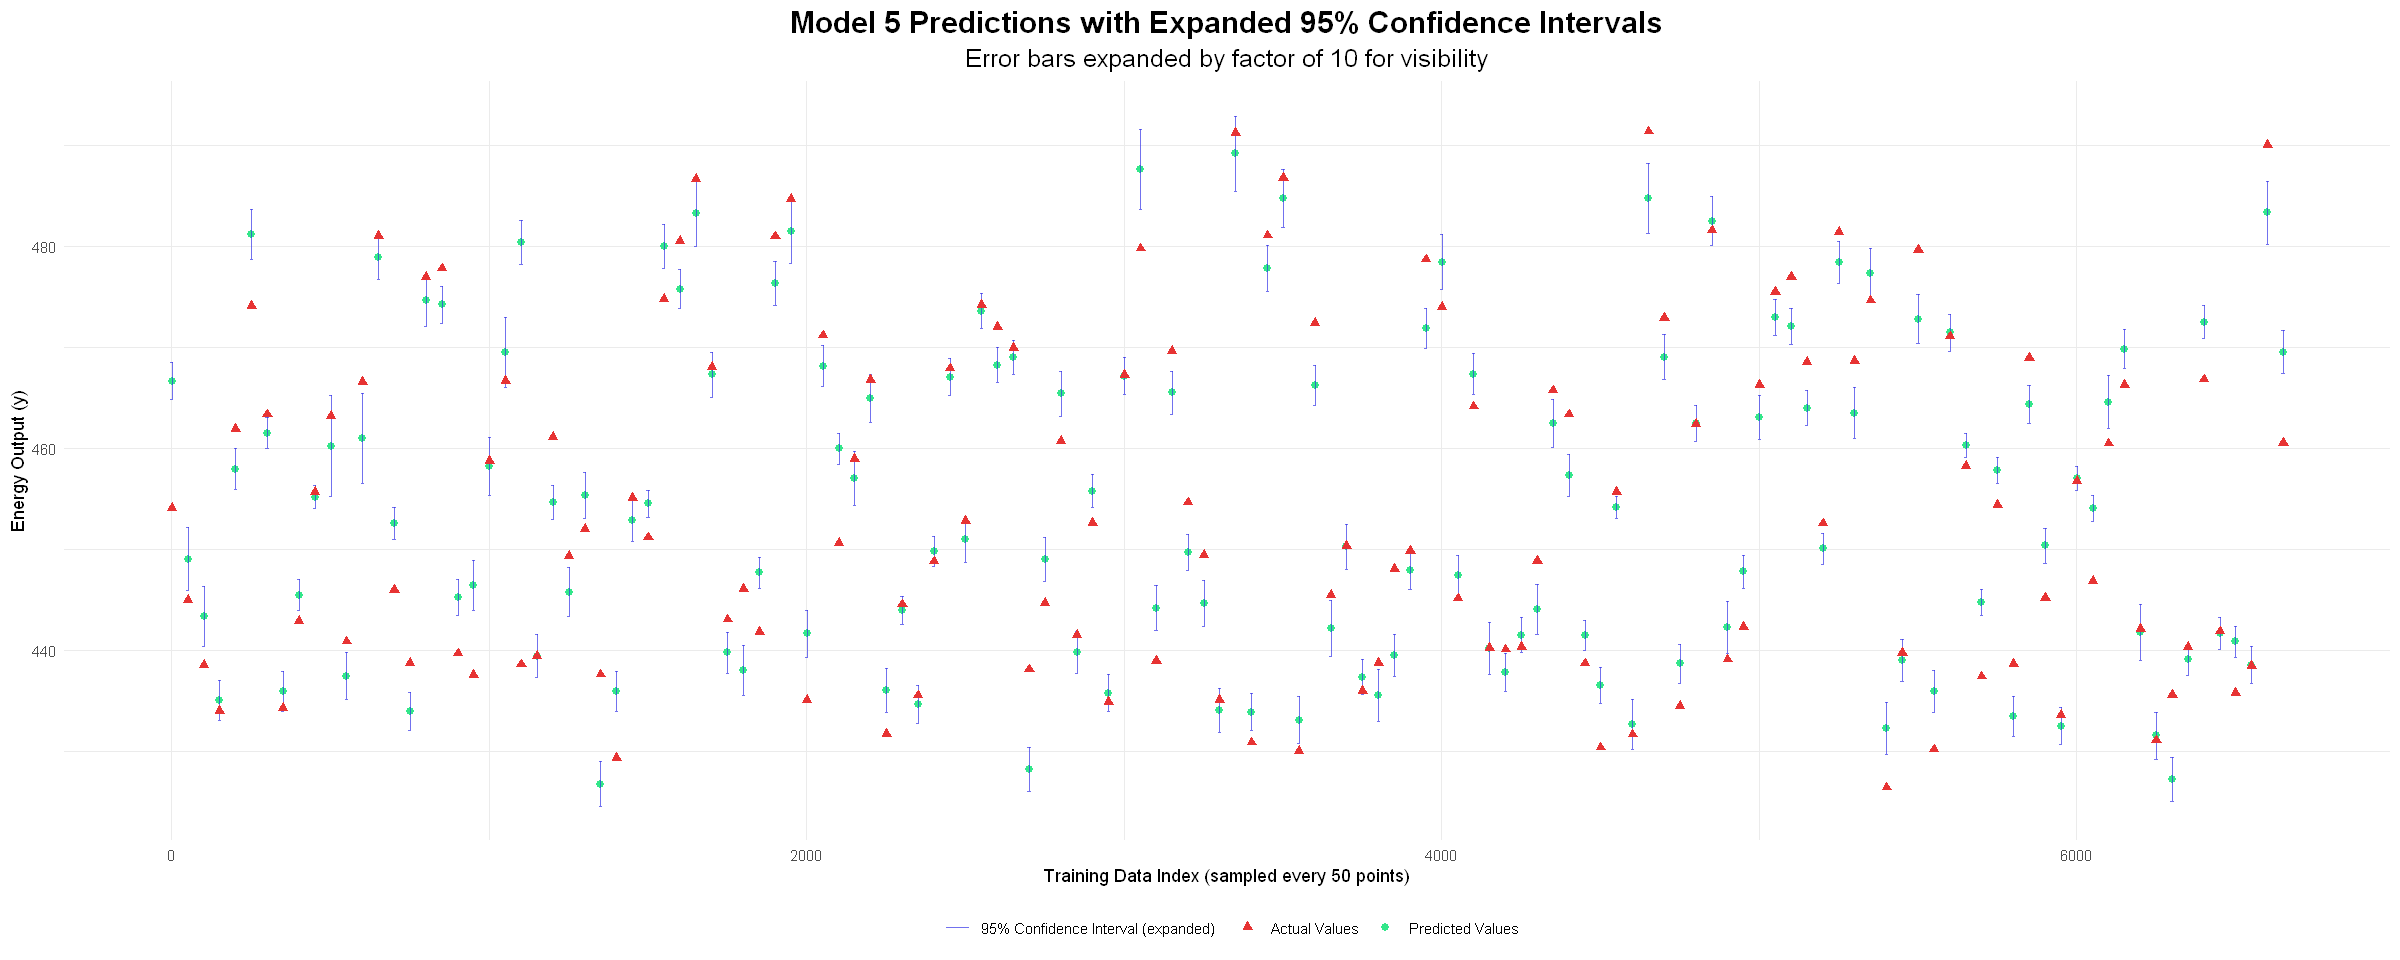
\includegraphics[width=\textwidth]{y19.png}
  %\caption{(Model-5 predictions with 95\% Confidence Intervals)}
  %\label{fig:Confidence Intervals}
\end{figure}

%This plot displays Model 5's predictions on the training data, 
%with the 95\% confidence intervals visually expanded for clarity. 
Green dots represent predicted values and the red triangles show 
the actual observed energy output. The blue error bars, scaled up 
ten times, highlights 95\% confidence intervals for predictions. 
Most actual values are close to the predictions, suggesting 
good model accuracy. Few red triangles lie outside the blue bars, 
indicating potential outliers or regions where the model's performance 
is less reliable.

\subsubsection*{Task 2.8.2: Evaluation on Testing Data}

The optimum model parameters from Task 2.7.1 were used to make predictions on the testing data. 
Distribution plots for actual and predicted values were then studied to analyze whether the model 
captures the overall structure of the data. 

\begin{figure}[H]
  \centering
  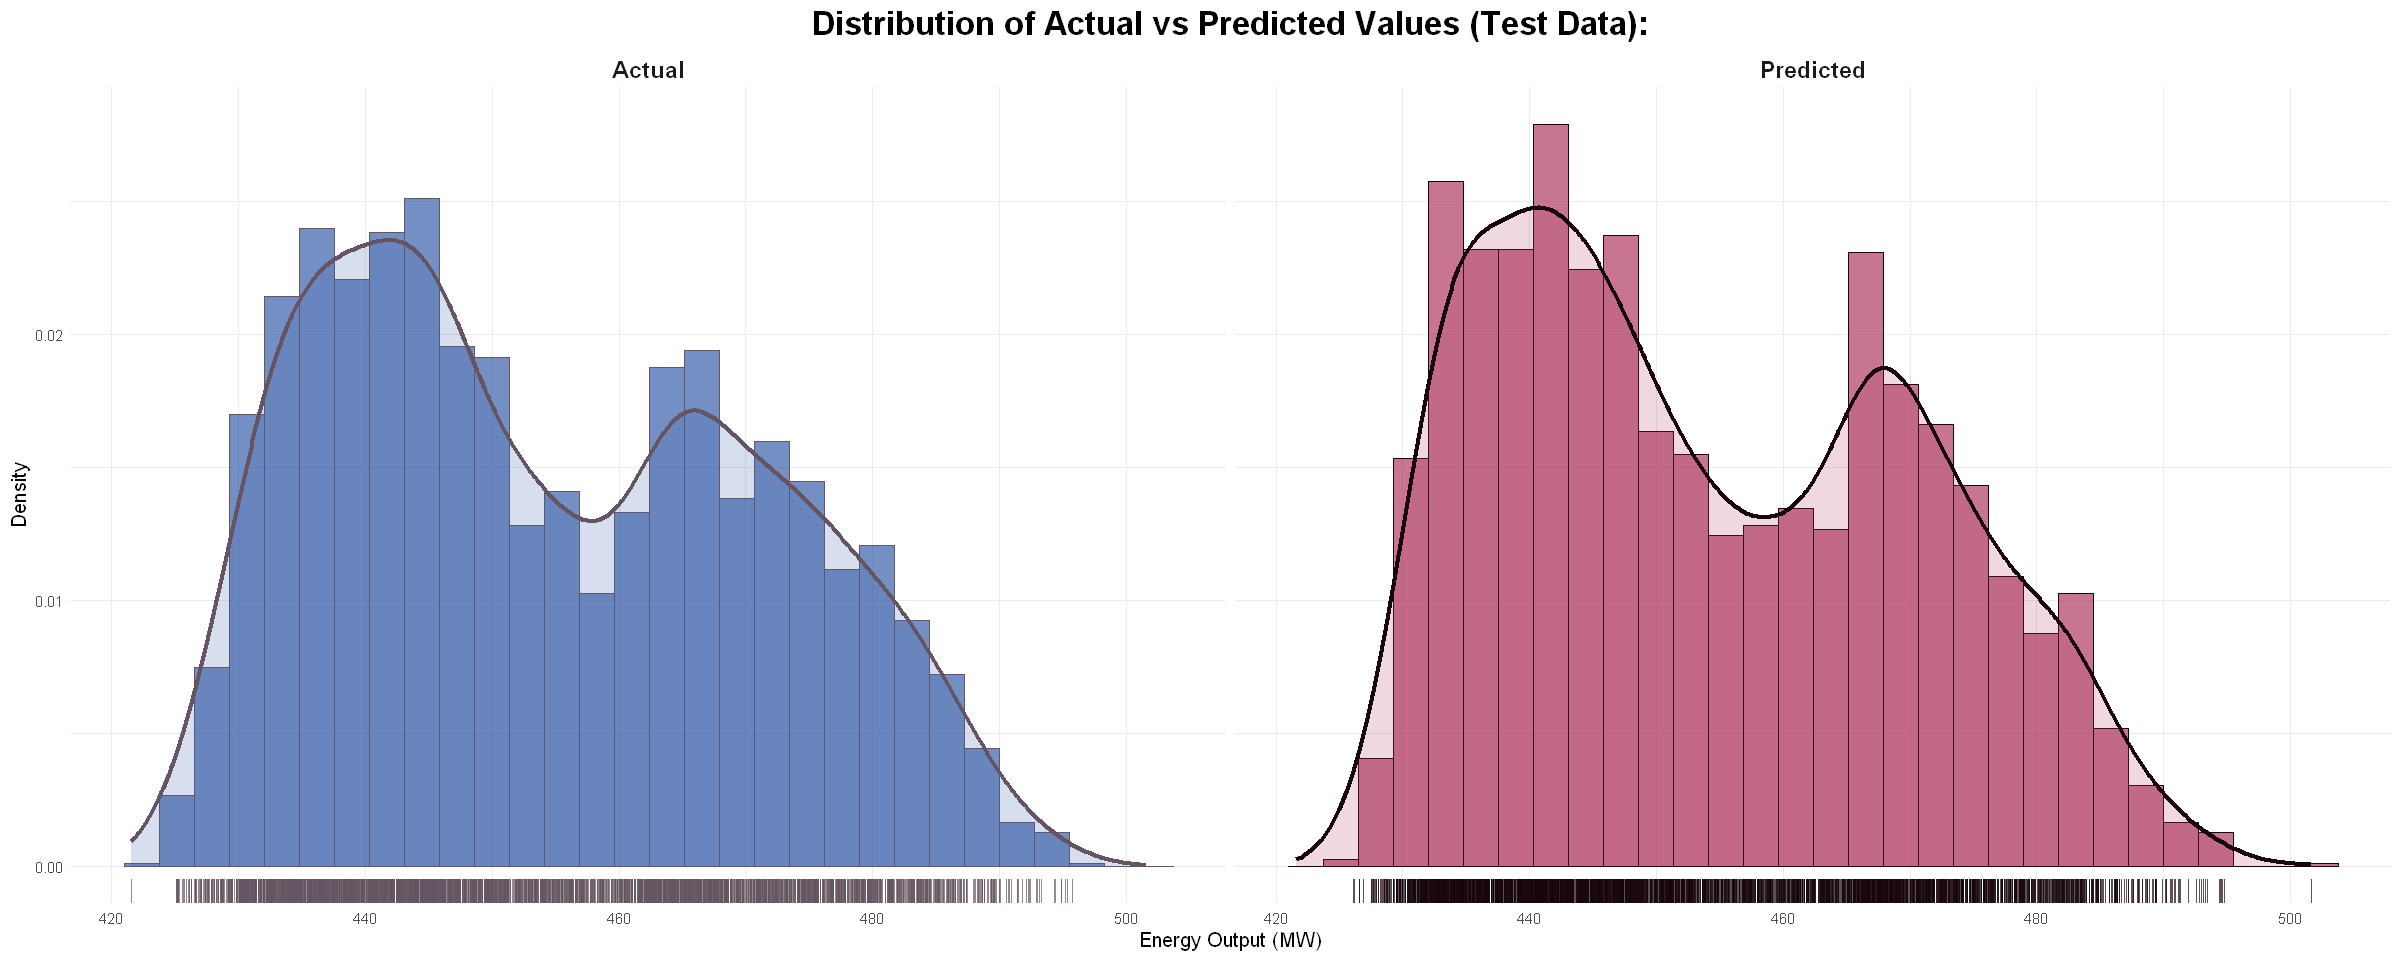
\includegraphics[width=\textwidth]{y20.png}
  \caption{(Distribution of Actual vs. Predicted Values for test data)}
  \label{fig:Actual vs. Predicted for testing data}
\end{figure}

Left curve shows the histogram (with density curve overlayed over it) for the actual values. 
The distribution is not symmetrical, it possess characterstics of
bimodal distribution. The rugplot at the buttom indicates the values are somehow distributed widely 
(between $430$ to $490$) along x-axis.

The distribution of predicted values for the testing dataset almost resembles with left curve (curve of actual values). 
The shape is not normal, this curve also possess the properties of bimodal distribution. 
Rug plot at bottom shows, the predictions are more centered around $430-490$
range. Both the curves are similar in shape and appearance indicating model is making
highly accurate predictions and because of high accuracy 
curves are almost identical. 

Also, the residual were calculated and their distribution was plotted to check for
their normality (a key assumption in Regression):

\begin{figure}[H]
  \centering
  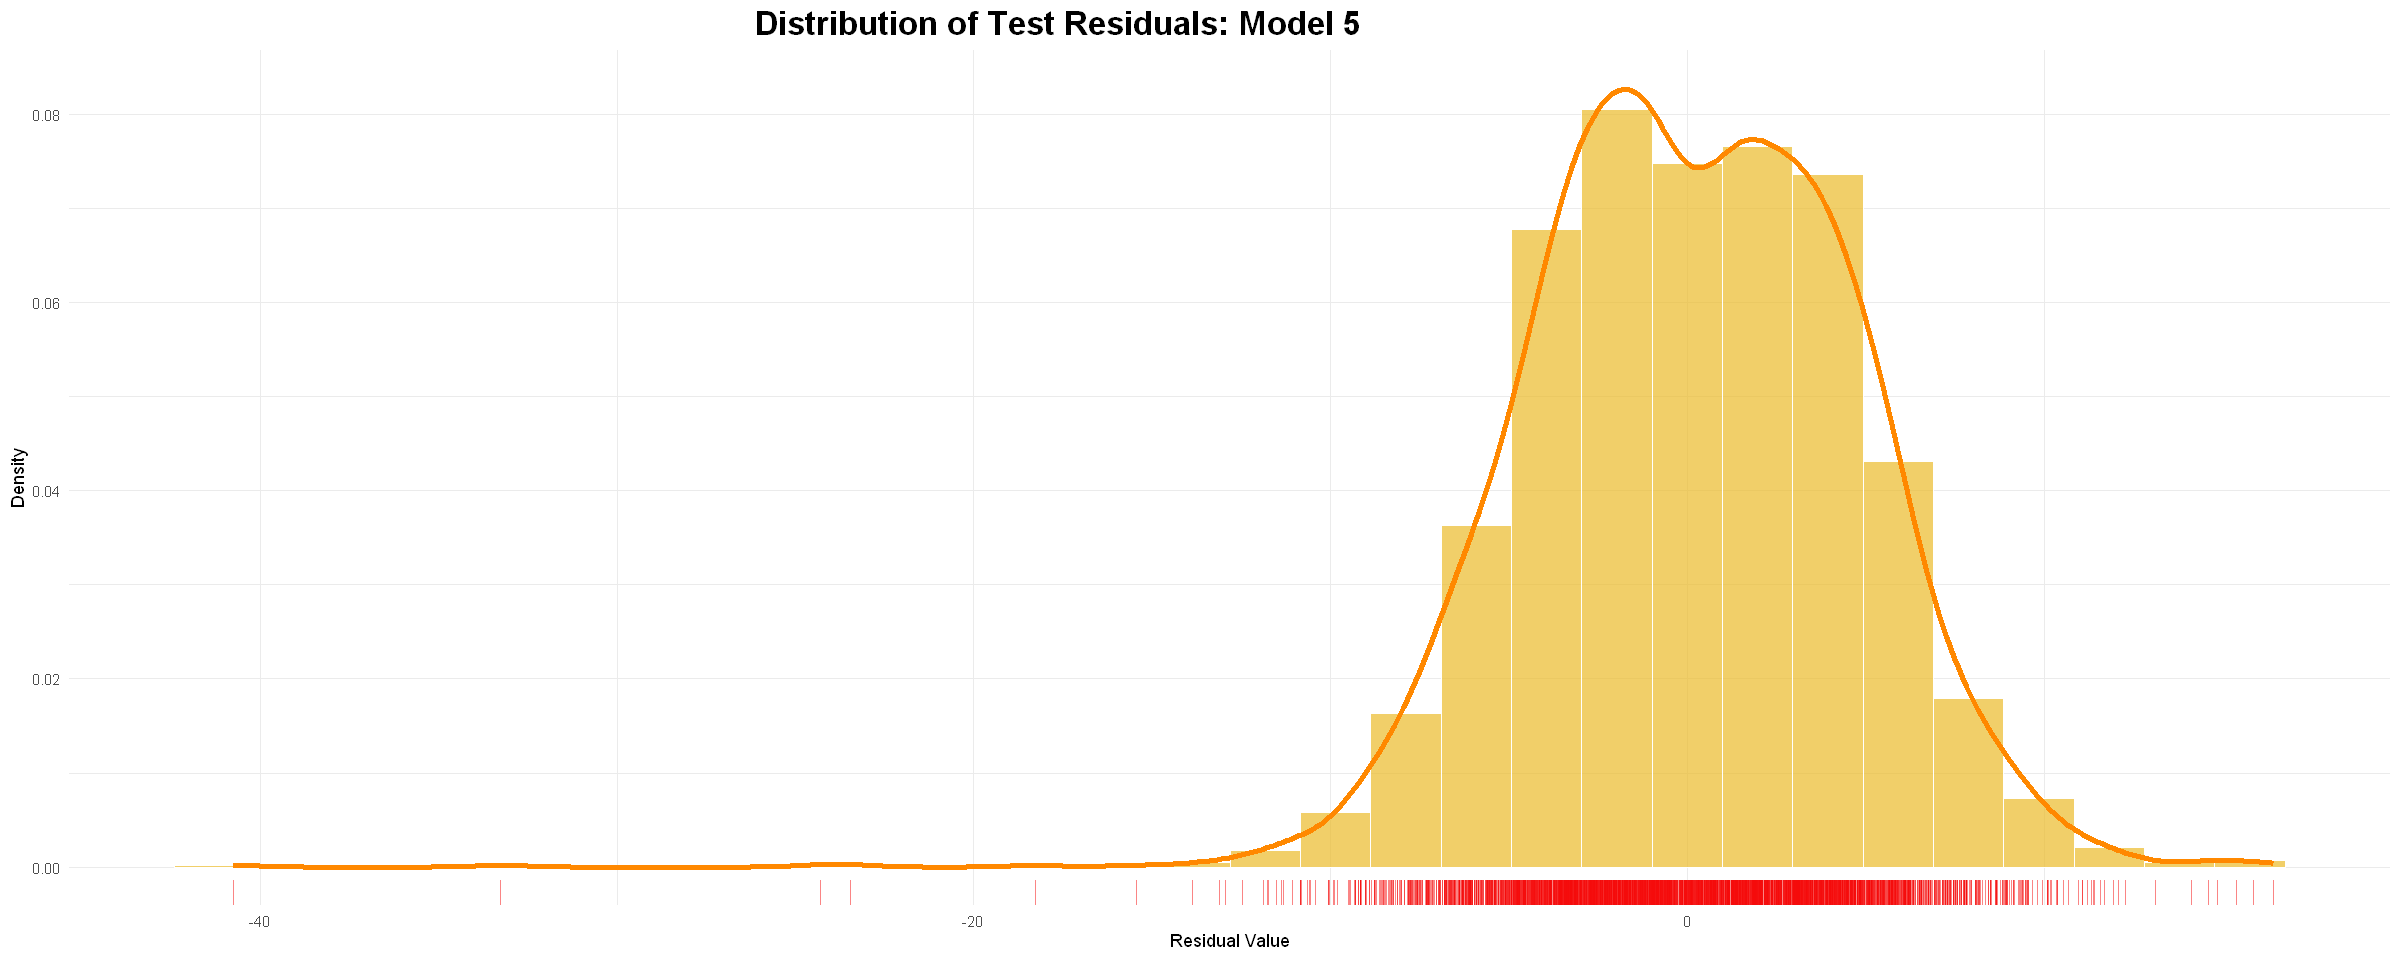
\includegraphics[width=\textwidth]{r21.png}
  \caption{(Normality of residuals for test data)}
  \label{fig:Distribution of residuals for testing data}
\end{figure}

%The plot shows the distribution of residuals calculated by taking difference between actual and 
%predicted values for test dataset. 
%Yellow bars represents the histogram of the residuals whereas the 
%orange line over the histogram is the density plot for the residuals. The red ticks at the 
%bottom are rug plots which shows the individual residuals.

Residuals are distributed around center zero ($mean= 0$) which indicates the model is unbiased. 
The distribution is almost symmetrical around zero with approximate bell-shape; excluding those five 
extreme residual values at the left tail. 
The distribution is acceptably normal which is the assumption in regression analysis. 
Model is performing well in the training dataset.

A comparison between predicted and actual values for test dataset was conducted
using scatter plot to check if they are close enough: 

\begin{figure}[H]
  \centering
  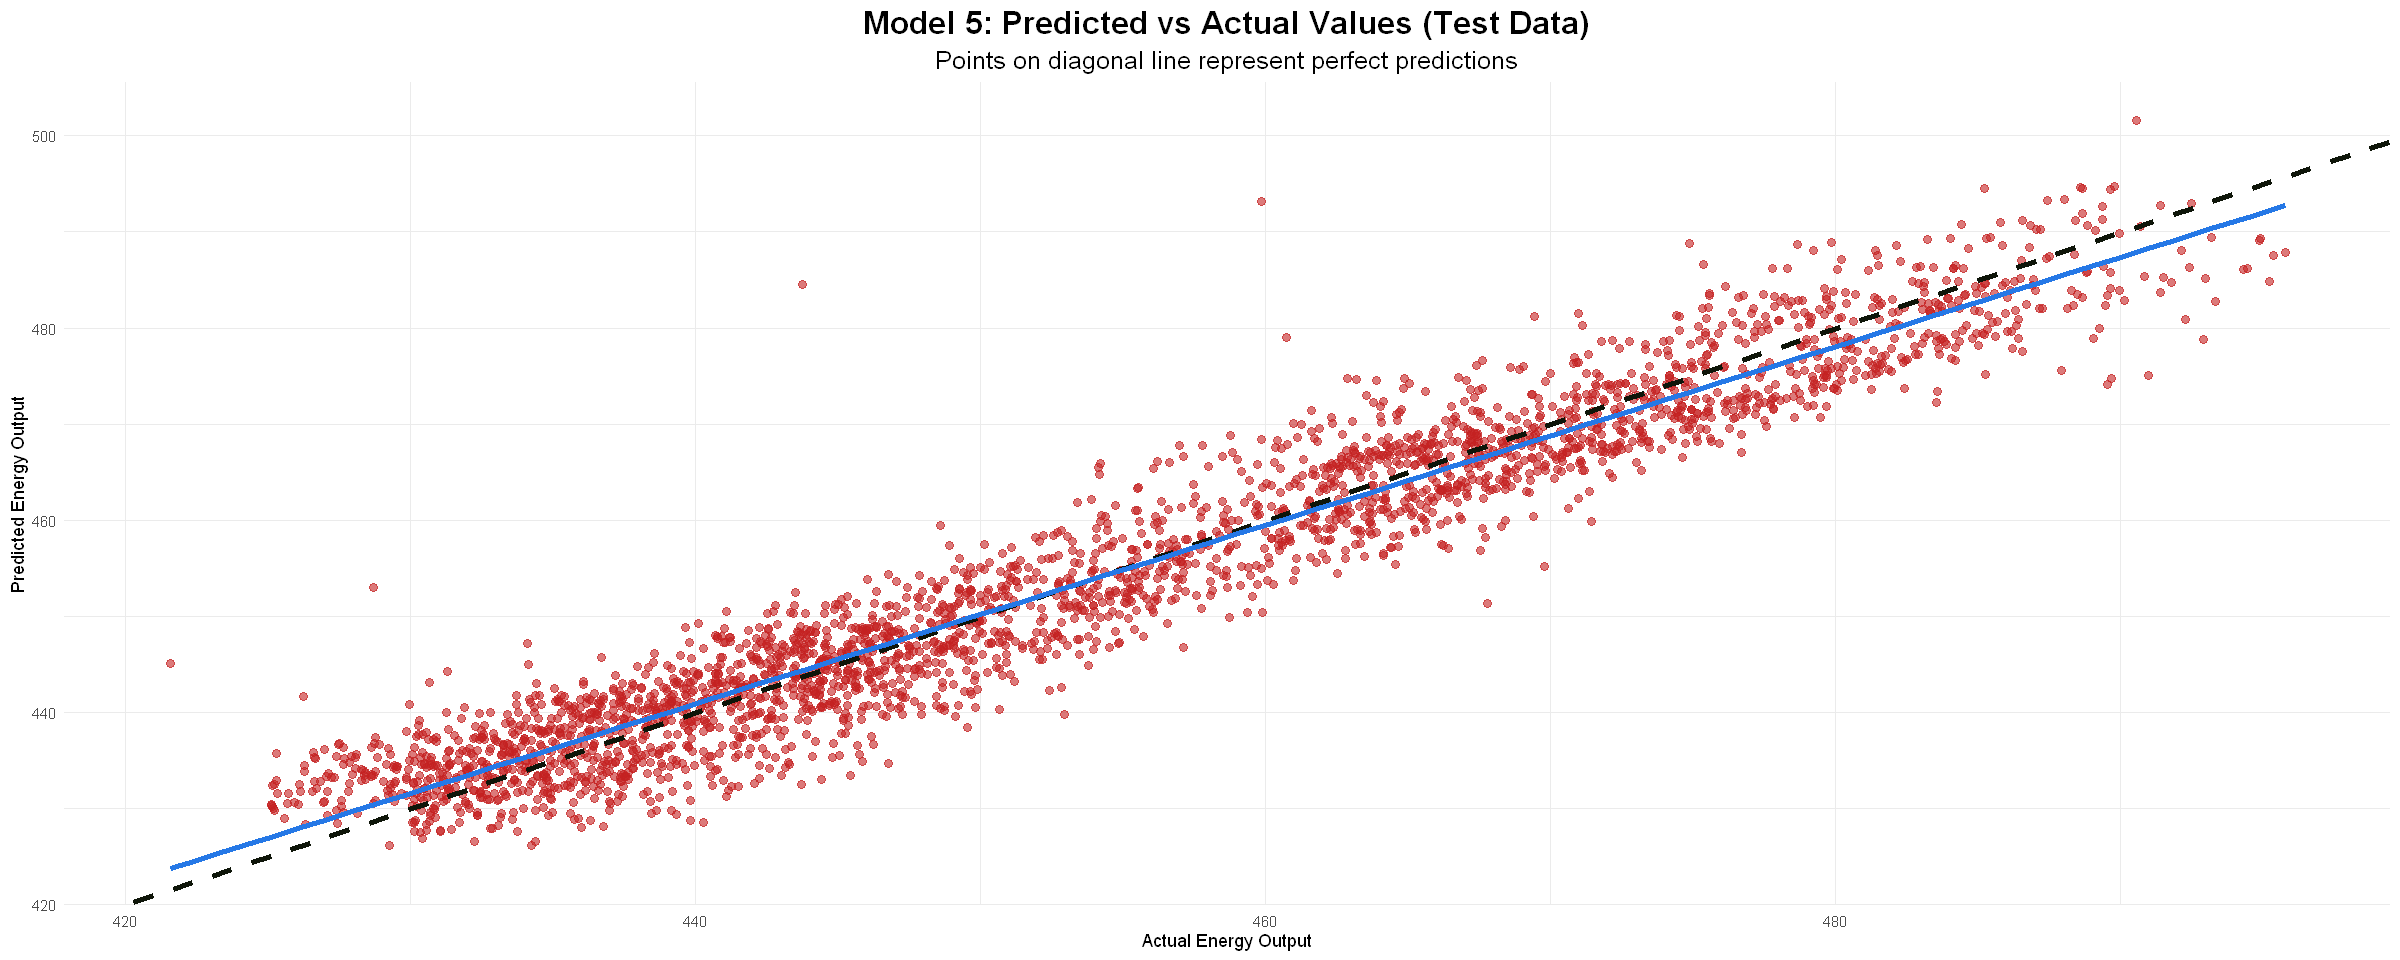
\includegraphics[width=\textwidth]{y21.png}
  \caption{(Predicted vs. Actual values for test data)}
  \label{fig:Comparision between predicted and actual values}
\end{figure}

%On x-axis, plot shows the actual enorgy output values and on the y-axis 
%it shows the predicted values for the testing dataset.
%A black dashed diagonal line is plotted which is a hypothetical perfect prediction line.
%The red dots on the plot are the actual values and more closer these 
%values to the diagnol line are, the more accuracy the predictions will be. A blue line is also plotted
%which shows an overall relation between predictions and the actual values. 

The general trend line (blue line) and the reference line (black dashed line) are parallel and almost
overlap on each other. Also, the actual values (red dots) are linearly clustered around the reference
line with constant variance. There are very few points on the curve which are randomly scattered. This 
is very accurate model with high percision. 

A through study on 95\% confidence interval were performed and found that the intervals are
quite narrow with mean width of about ($0.4207347$) , maximum width of about ($1.301707$) , and 
minimum width of ($0.2222644$). Narrow confidence intervals means model is making predictions with 
high level of ceretainty. To make error bars and CI visible, I zoomed-in the y-axis by a certain factor. Zooming y-axis 
may results into cutting-off the values from the screen frame but this is only for visualization purpose: 

\begin{figure}[H]
  \centering
  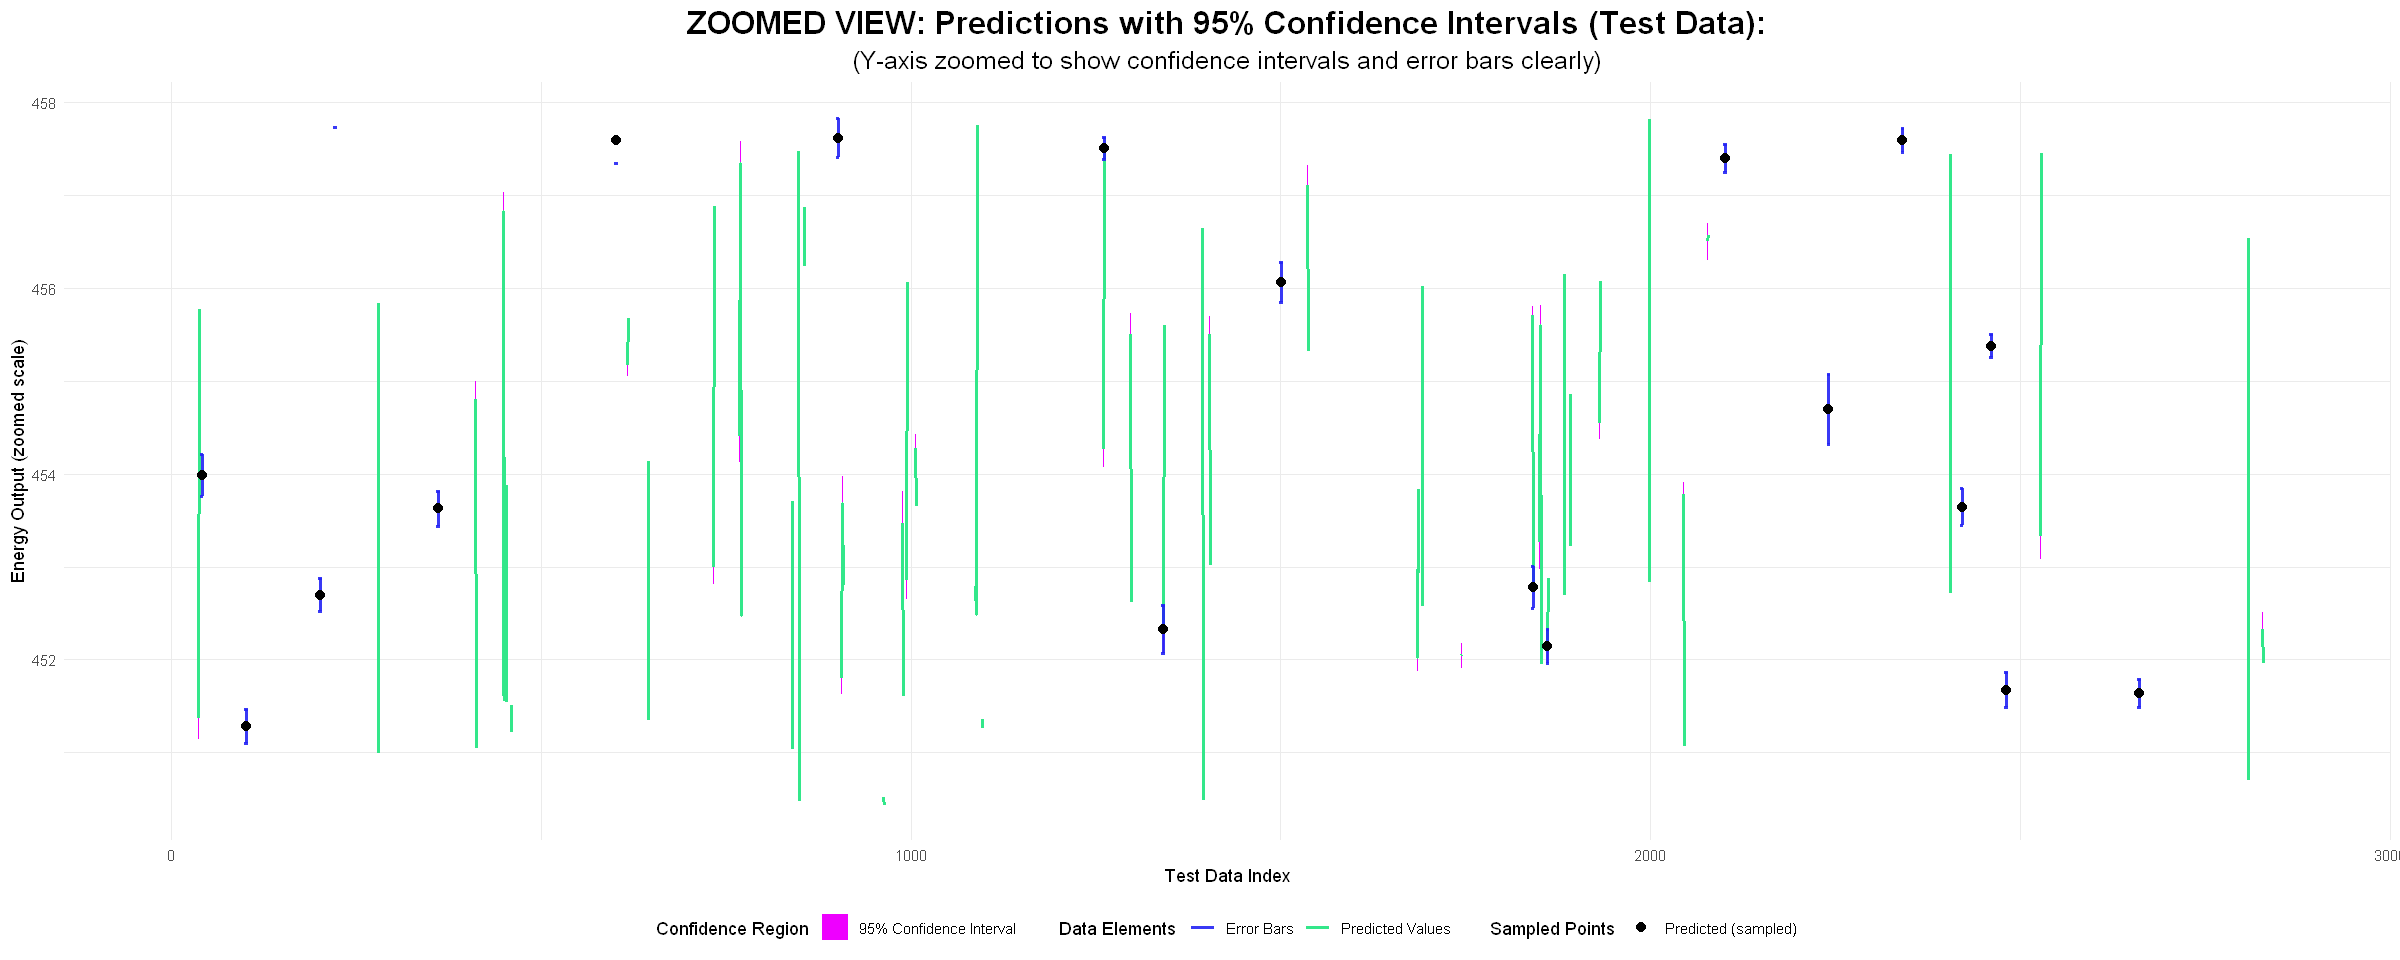
\includegraphics[width=\textwidth]{y22.png}
  \caption{(95\% Confidence Interval with Error Bars (Zoomed y-axis))}
  \label{fig:CI for testing data with Error Bars}
\end{figure}

%Model's predictions on the test dataset are displayed in this graphic 
%together with error bars and 95\% CIs. The black dots are 
%sampled anticipated spots, and the green line shows the expected energy output.  
%The range that the genuine energy output is predicted to fall inside with 95% 
%certainty is shown by the pink confidence interval ribbons and the blue error bars 
%(for every 20th point). 
Even after zooming the y-axis, the confidence intervals and
error bars are still very narrow and requirs through investigation to see them properly.

A small sample of 16 data points ($100-115$) was choosen and plotted to visualize how
narrow our Confidence Intervals for the predictions were:

\begin{figure}[H]
  \centering
  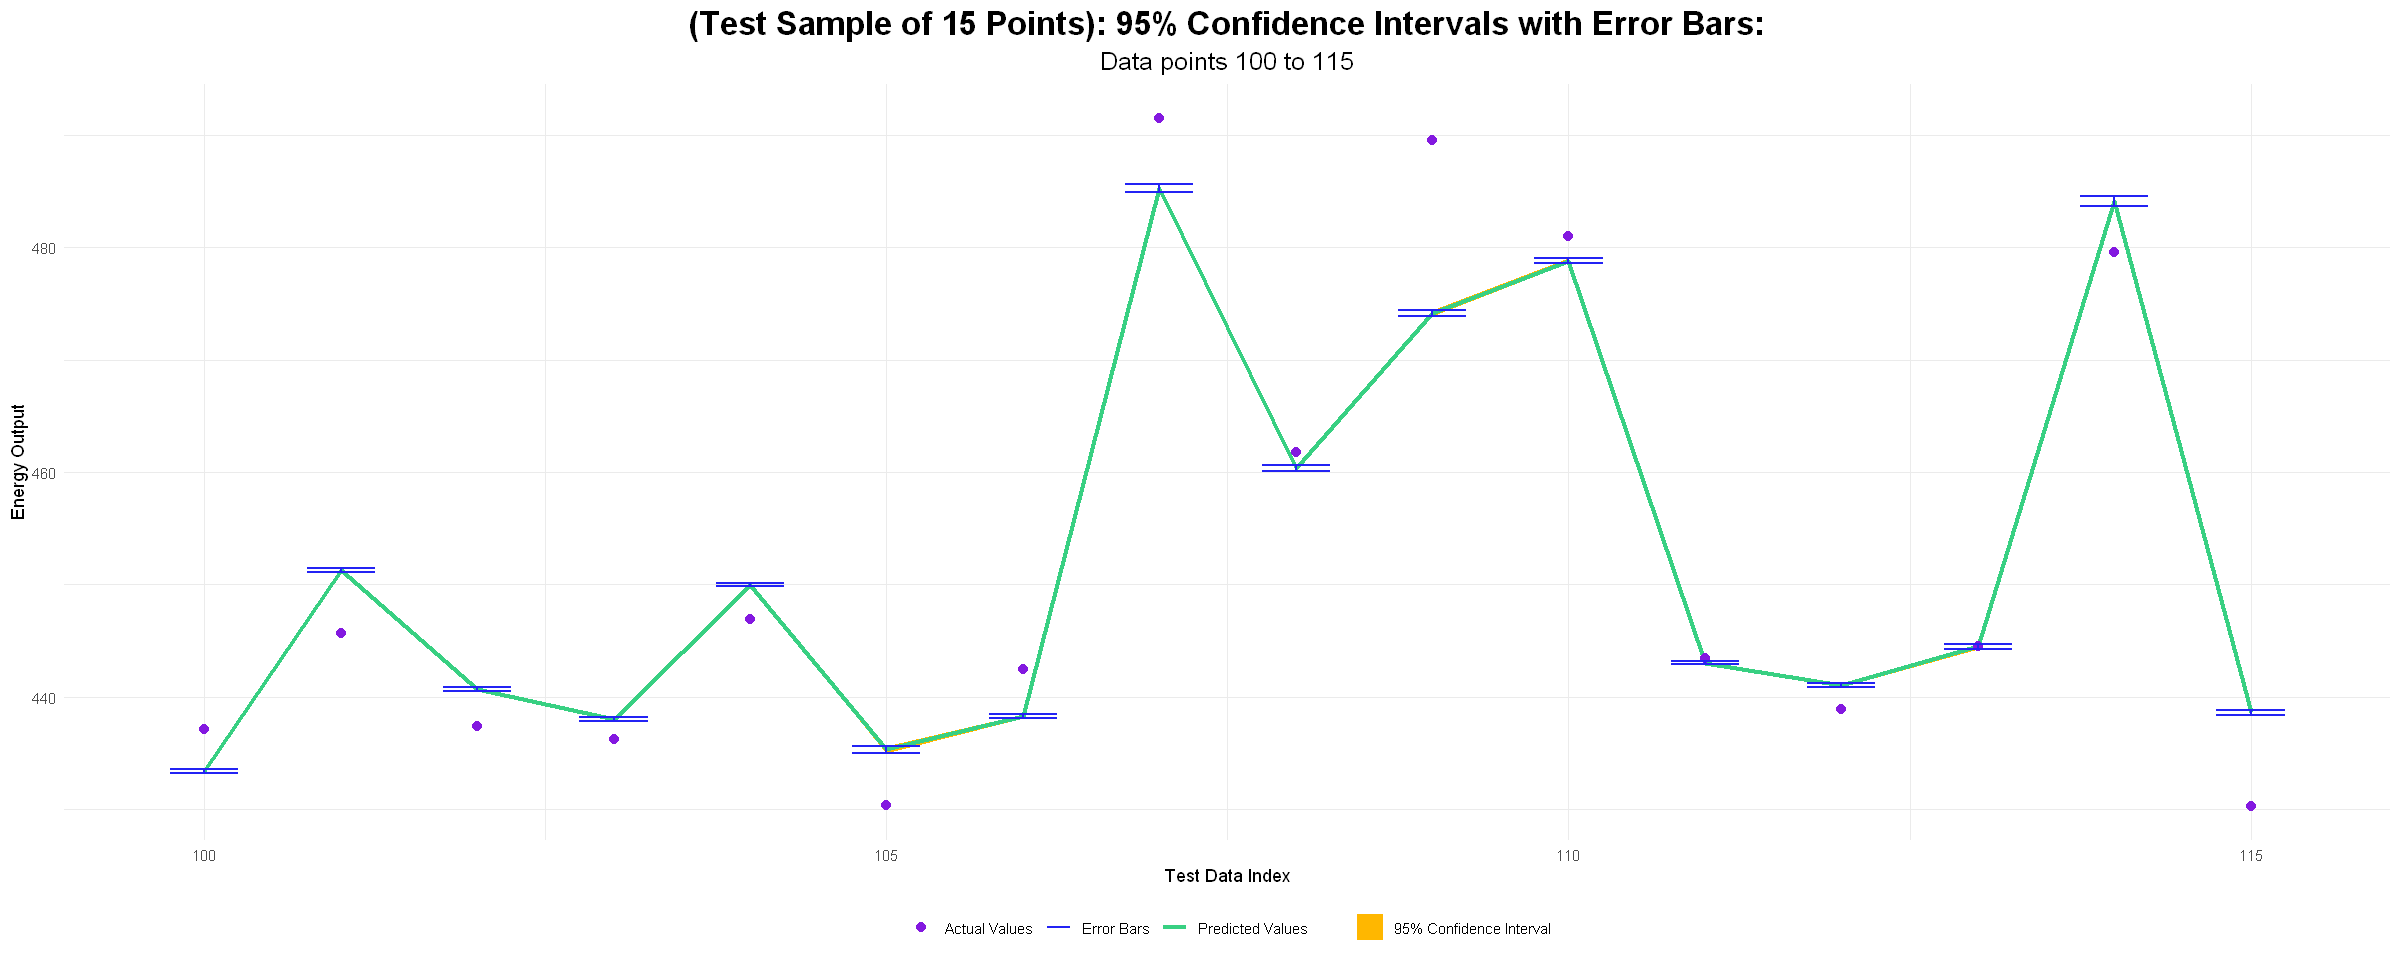
\includegraphics[width=\textwidth]{y23.png}
  \caption{(95\% Confidence Interval with Error Bars for 16 data points)}
  \label{fig:CI for testing data with Error Bars for 16 data points}
\end{figure}

%In this plot, purple dots scattered around the curve are the actual values, blue ribbon represents the
%width of confidence interval and the green line represents the line that joins the predicted values.
Error bars are denoted by blue marks which shows how narrow they are compare to the 
full range of energy output values. The intervals appear very thin and only cover less then 1\% 
of the total range. 

So, our model 5 is performing well on both training data as well as on the testing datasets. Predictions are 
very accurate with very narrow confidence intervals where predictions almost resembles the true values. 

%----------------Task 3-----------------------

\section*{Task- 3: Approximate Bayesian Computation}
ABC is used when we want to do basian inference; 
instead of calculating the likelihood, we simulate data
from our model and compare with the real data. In ABC, 
we first guess a value for the parameter, 
then, we use that value to simulate the data. Then, we compare 
the simulated data with real data. If the simulated data 
is close enough, we accept the parameter. We repeate this 
process many times to build the posterior distribtion. 
%"Close Enough" is generally used as distance function 
%and a tolerance thresold. ABC helps us when models are complex 
%or want to support the traditional OLS results by 
%simulating the data.

Our chosen model was Model-5: 
\[y = \theta_1 \cdot x_4 + \theta_2 \cdot x_1^2 + \theta_3 \cdot x_3^2 + \theta_{\text{bias}}\]
%where the optimized model parameters we obtained from Task 2.1 are: 
%\[
%\theta_{\text{bias}} = -754.486865,\quad 
%\theta_1\ (x_4) = 186.436251,\quad 
%\theta_2\ (x_1^2) = -4.728874,\quad 
%\theta_3\ (x_3^2) = -2.599210
%\]

\begin{figure}[H]
  \centering
  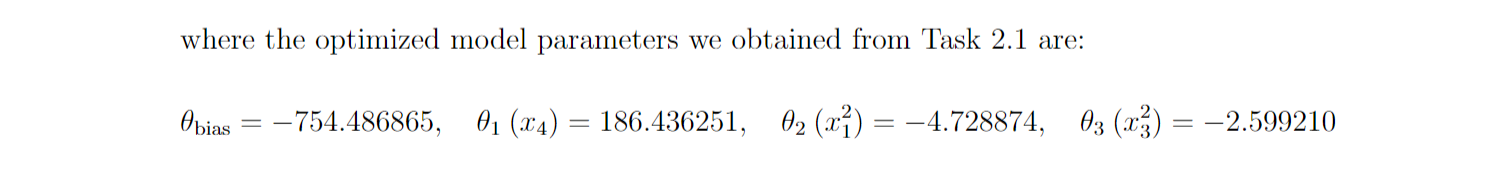
\includegraphics[width=\textwidth]{t1.png}
  %\caption{}
  %\label{fig:}
\end{figure}

\subsection*{Varying $\theta_1$ and $\theta_2$}

Two parameters having higest absolute values were selected for constructing the
posterior distribution where, other parameters were kept fixed. 
Uniform distribution was used to construct the prior distribution for the selected parameters 
$\theta_1$ and $\theta_2$ within $20\%$ around those values. Appropriate sample size and acceptance thresold were choosen to perform ABC rejection sampling  
to simulate the real data for $\theta_1$ and $\theta_2$. 

Posterior distribtion for parameter $\theta_1$ was
plotted and graph obtained is shown in the 
following figure:

\begin{figure}[H]
  \centering
  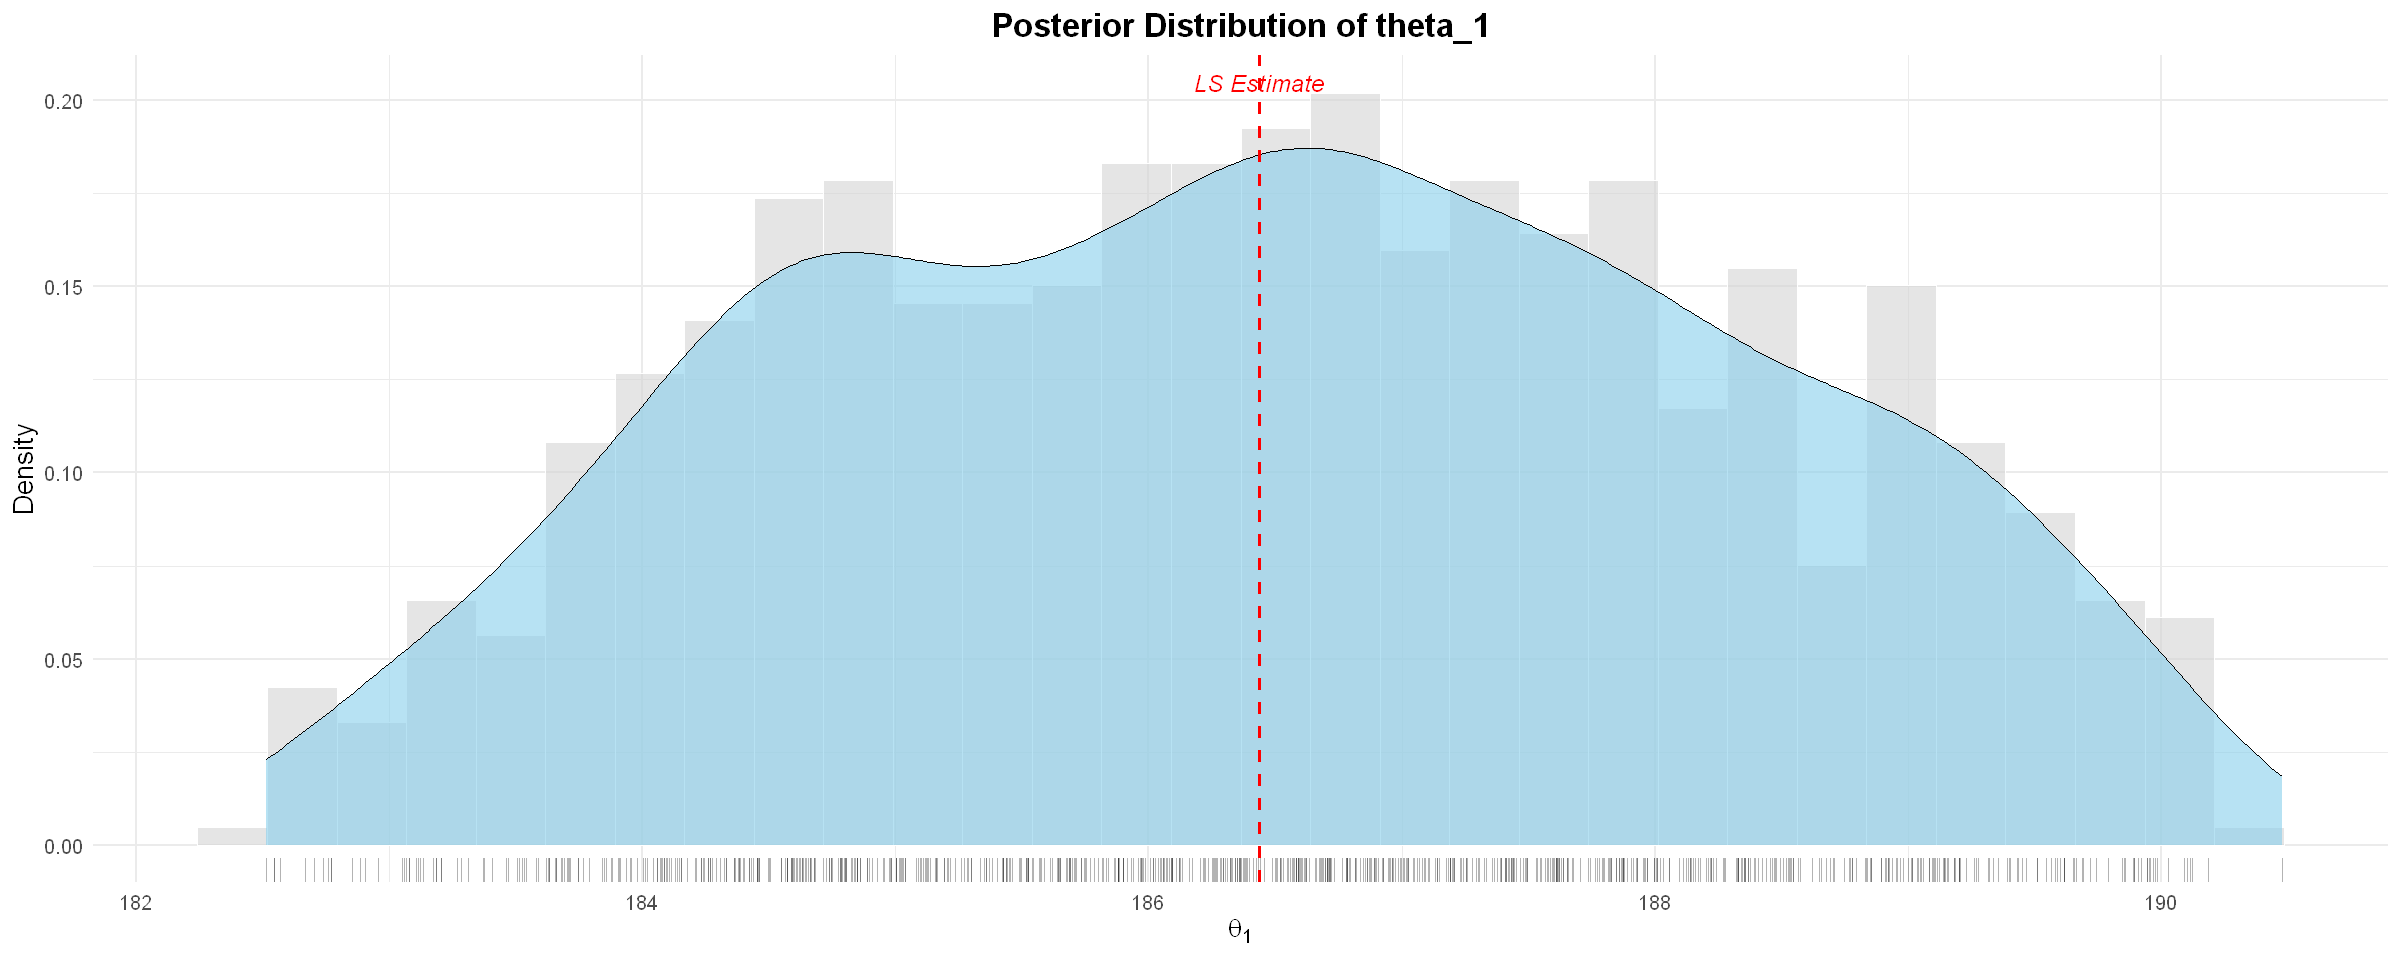
\includegraphics[width=\textwidth]{m7.png}
  \caption{(Posterior Distribution of $\theta_1$)}
  \label{fig:Posterior Distribution of theta_1}
\end{figure}

The distribution is almost bell-shaped and symmetrical, 
having the Least Squares ($LS= 186.43$) estimate value near its center.
The majority of the backbone's mass is located in a small range, 
indicating a high level of parameter estimation confidence. The ABC posterior supports the 
LS estimate, with little evidence for values 
far from the LS solution. 

Plotting of the posterior distribution 
for parameter $\theta_2$ produced the graph that is displayed in the following figure:


\begin{figure}[H]
  \centering
  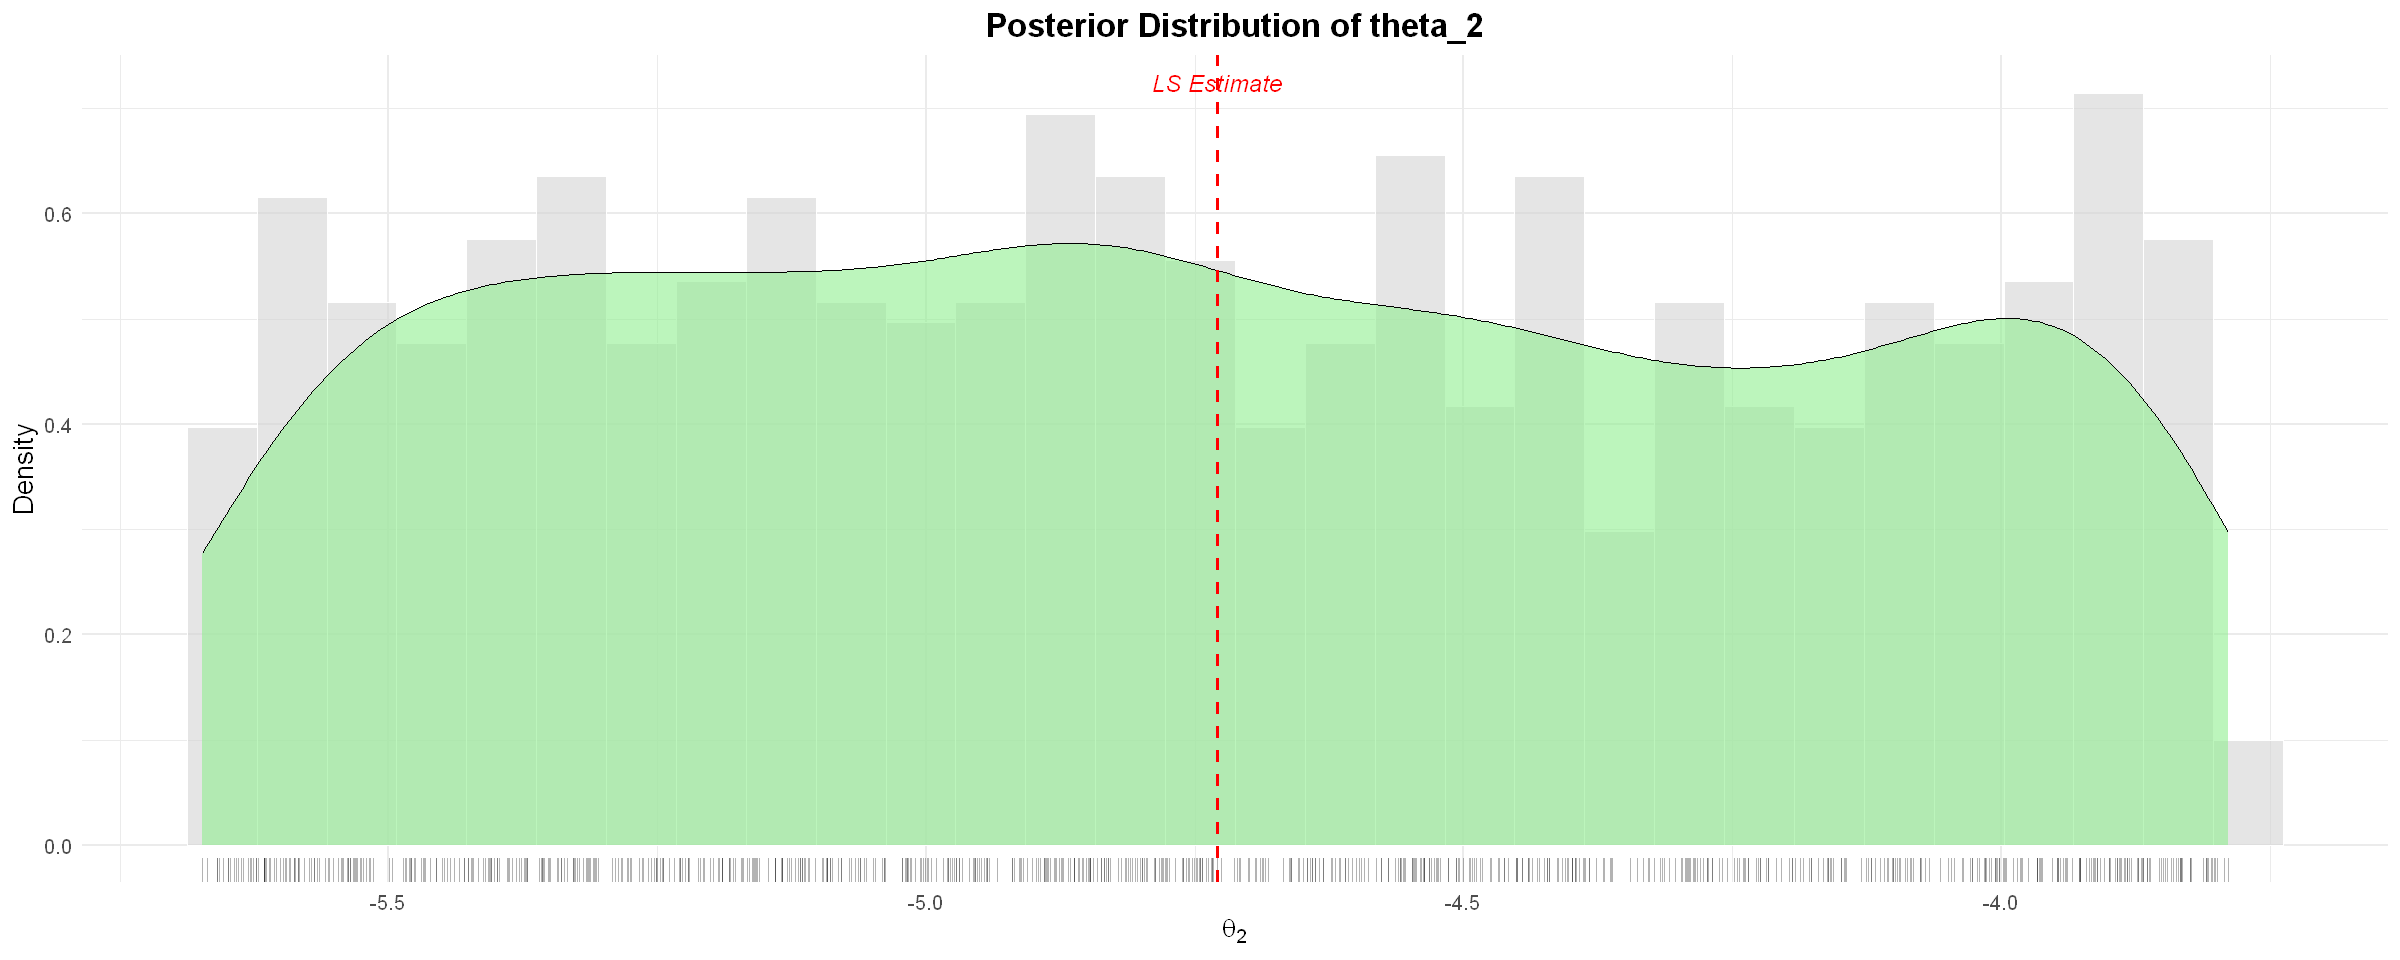
\includegraphics[width=\textwidth]{m8.png}
  \caption{(Posterior Distribution of $\theta_2$)}
  \label{fig:Posterior Distribution of theta_2}
\end{figure}

This distribution is neary flat almost like a uniform type of curve as ($\theta_2$ values ranges for a wide range of values), 
an indication of high uncertainty for $\theta_2$. The posterior is spread 
widely around the least square estimate value for $\theta_2$. 
The distribution suggests many values for $\theta_2$ 
are acceptable. The data provides very little information to 
preciously estimate $\theta_2$. 

A joint posterior distribution for $\theta_1$ and 
$\theta_2$ is plotted for both accepted and rejected 
posterior samples:

\begin{figure}[H]
  \centering
  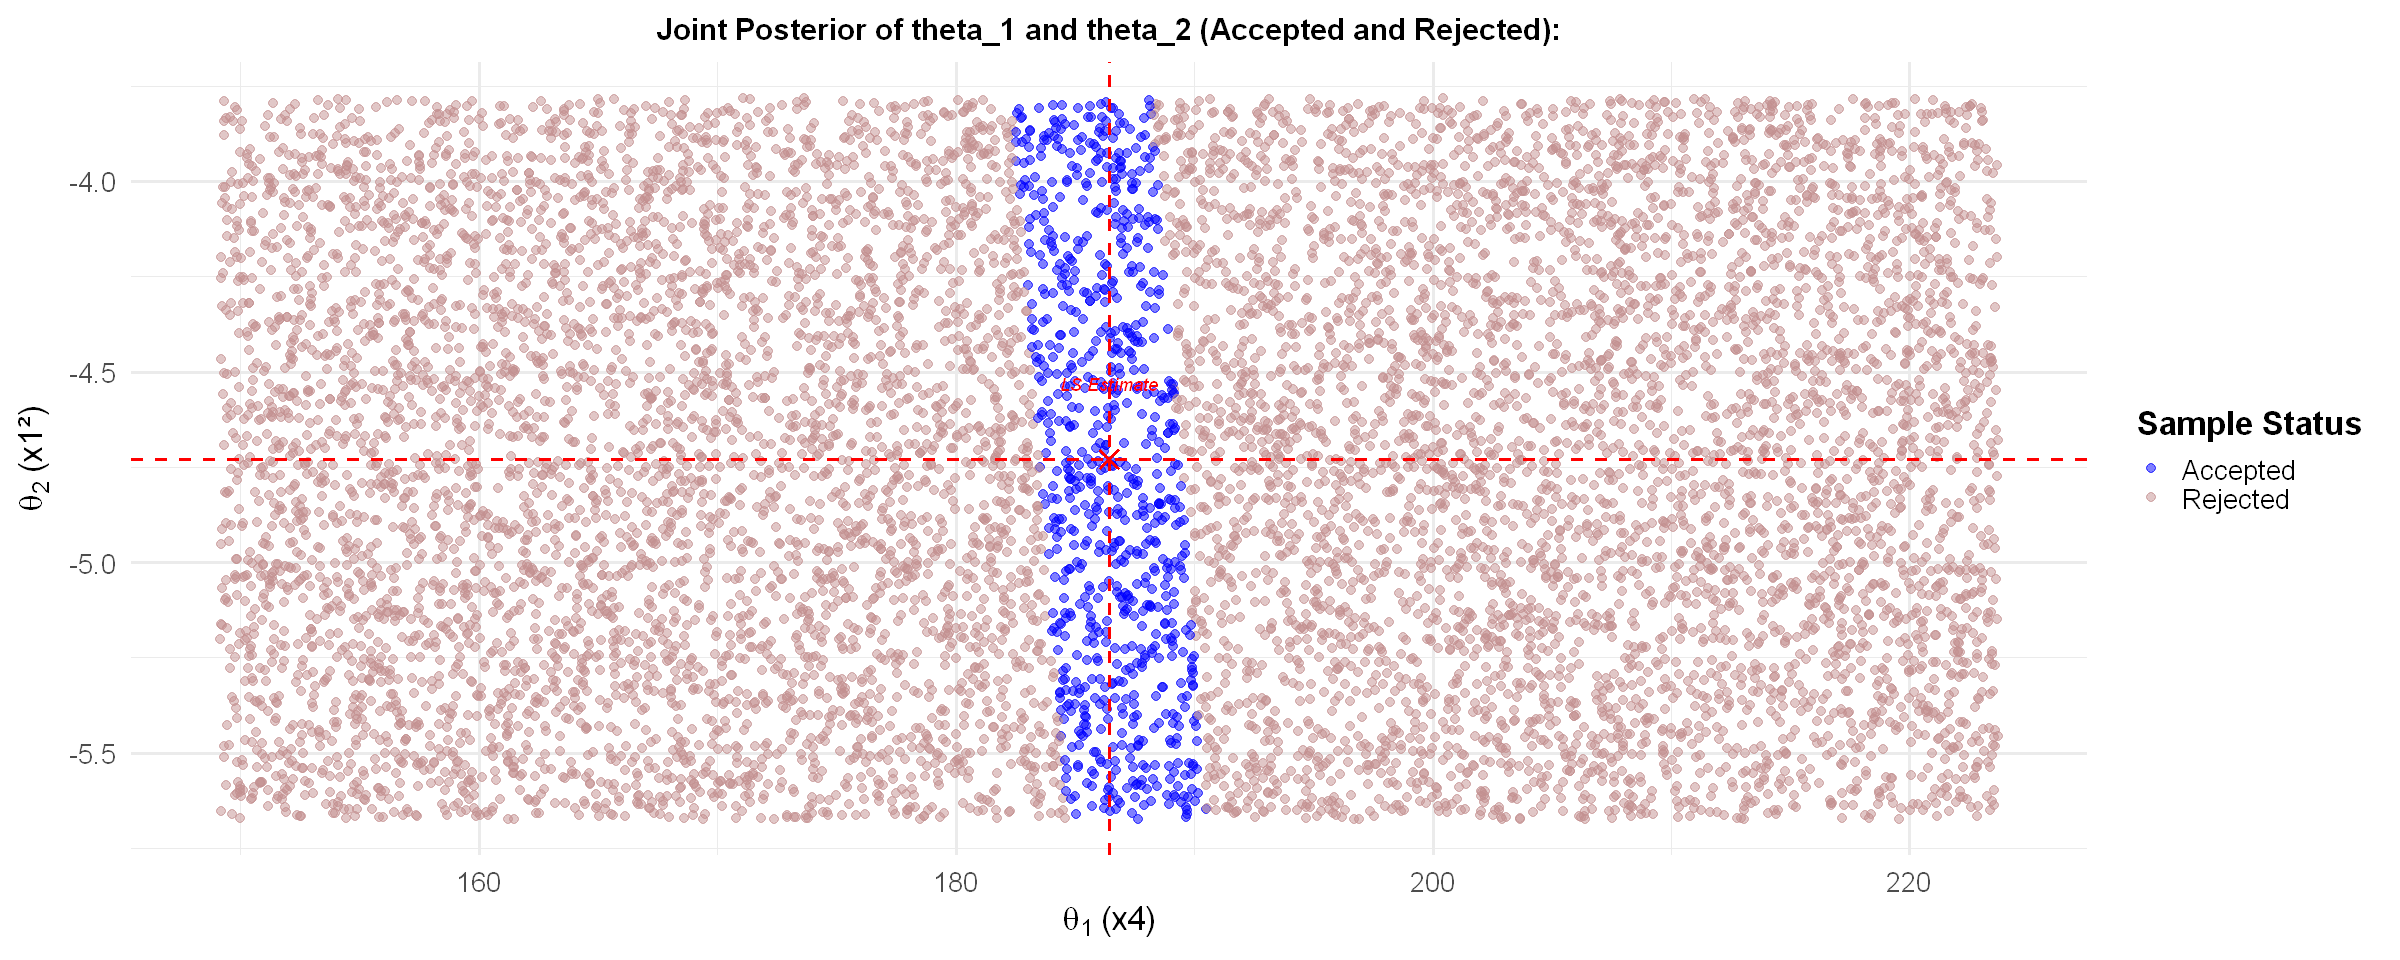
\includegraphics[width=\textwidth]{y27.png}
  \caption{(Joint Posterior of $\theta_1$ and $\theta_2$ (accepted + rejected))}
  \label{fig:Joint Posterior of $\theta_1$ and $\theta_2$}
\end{figure}

The accepted samples form a narrow vertical band ($\theta_1 = (183 - 190)$)
arond the Least Squares line indicating only a 
limited range of $\theta_1$ values produce good model 
fit. The effect of $\theta_2$ is much less certain and many 
vales (the limit for $\theta_2$ values is open as seen from the joint 
distribution indicating an uncertain range of values) of $\theta_2$ can 
fit the observed data. 

\subsection*{Fixed $\theta_1$ and $\theta_2$}

Now, ABC estimation is performed by varying $bias$ and $\theta_3$, 
keeping $\theta_1$ and $\theta_2$ fixed. Joint posterior distribution obtained 
for accepted samples is shown below: 

\begin{figure}[H]
  \centering
  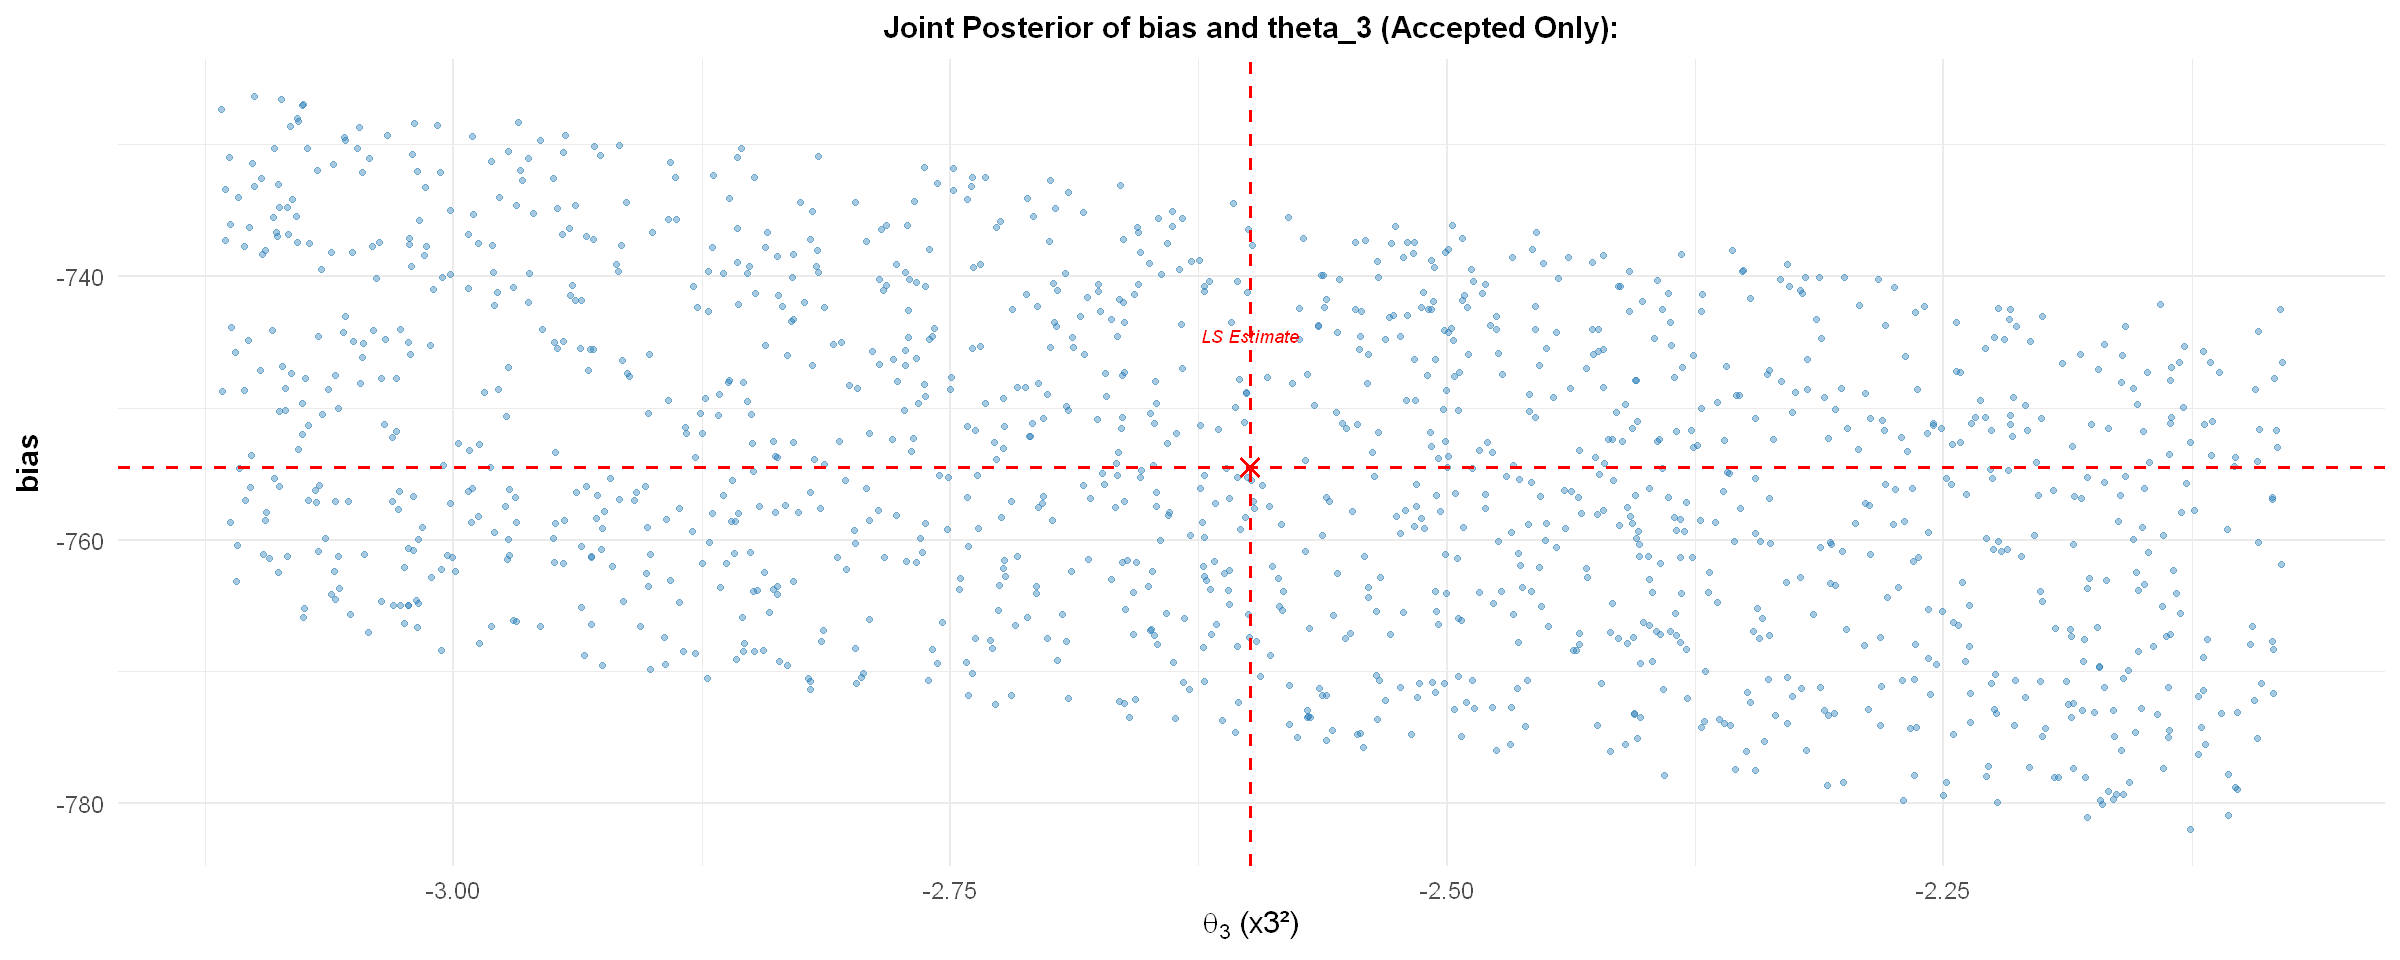
\includegraphics[width=\textwidth]{m10.png}
  \caption{(Joint Posterior of $bias$ and $\theta_3$ (accepted only))}
  \label{fig:Joint Posterior of $bias$ and $\theta_3$}
\end{figure}

There is no clear relationship or pattern between $bias$ 
and $\theta_3$; accepted values are scattered in a rectangle.  
The LS ($bias$ = -754.49, $\theta_3$ =-2.60) estimates 
(red lines) are in the center of the accepted region, 
showing that the LS solution is supported by the Bayesian approach.  

Many combinations of $bias$ and $\theta_3$ fit the 
data well, and the model is not very sensitive to 
small changes in these parameters within the accepted range.

\begin{figure}[H]
  \centering
  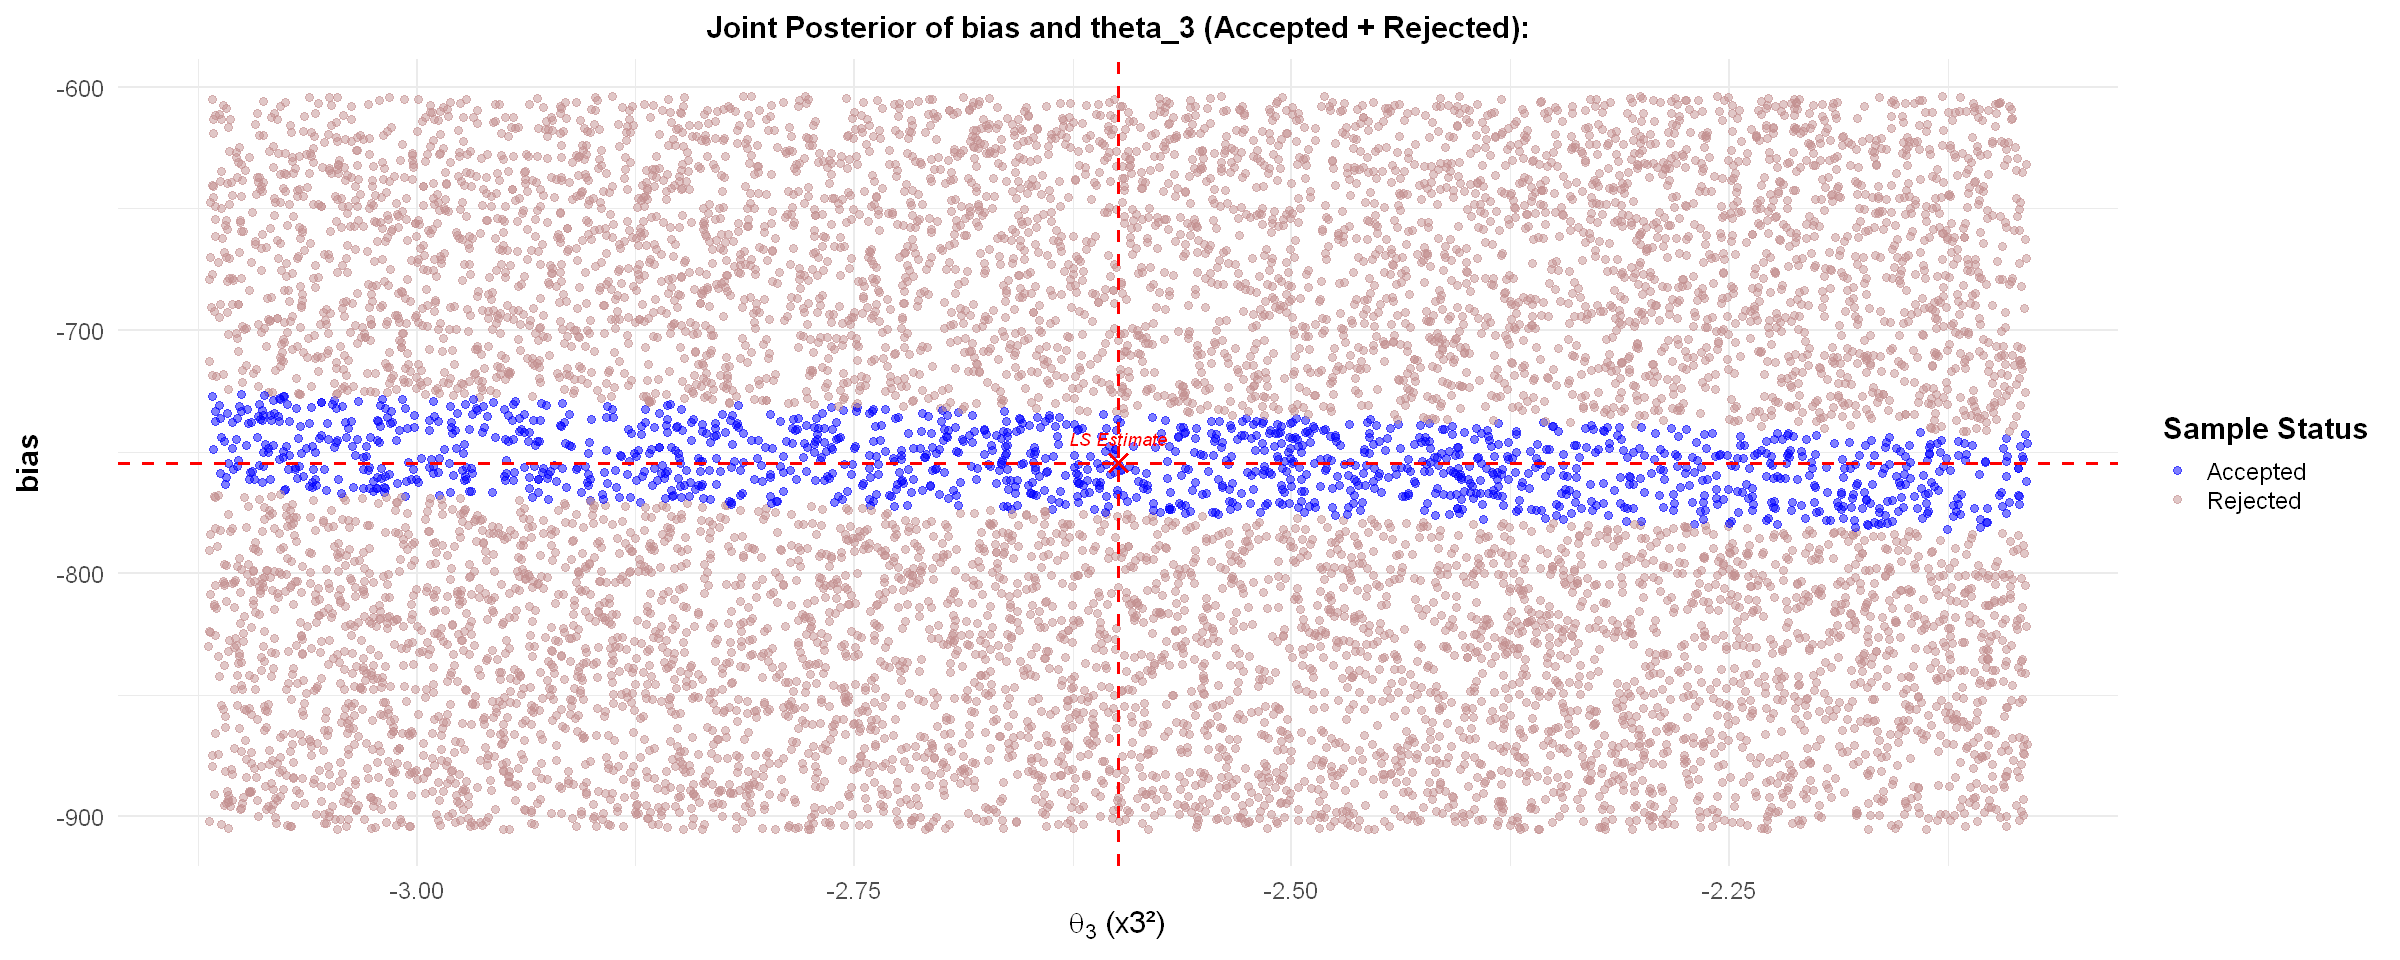
\includegraphics[width=\textwidth]{m11.png}
  \caption{(Joint Posterior of $bias$ and $\theta_3$ (accepted + rejected))}
  \label{fig:Joint Posterior of $bias$ and $\theta_3$}
\end{figure}

Accepted samples (blues) are tightly clustered horizontally 
from about $\theta_3$ = $-3.12$ to $-2.08$ and vertically from 
about $bias$ = $-905$ to $-603$. Rejected samples (brown) fill the 
rest of the rectangle, showing that most combinations do not fit 
the data well.  

There is no visible relationship between $bias$ and $\theta_3$; 
accepted values form a horizontal band. The LS estimates are in 
the center of the accepted region, confirming the LS solution is 
supported by the Bayesian approach. 

Only a narrow range of $bias$ values (around $-754.49$) with a 
wide range of $\theta_3$ values fit the data well, and the model 
is not sensitive to $theta_3$ within this accepted range.

%--------------------------------------Limitations------------------------------------

\section*{Limitations}

While this study provides a  well performing regression model 
for predicting power plant energy output, some limitations of the study 
should not be ignored. First, this analysis is based on historical data 
generated from a powerplant, which certainly limits generalizability to other 
plants or regions. Second, the model assumes that relationships 
between variables remain stable over time; any structural changes or 
unmeasured factors could affect predictive accuracy. Third, 
although the model performs well on available data, it may not 
capture rare or extreme operational conditions not present in the 
dataset. Finally, the uncertainty present in some parameter estimates 
(e.g., squared temperature effect) suggests that further data or 
alternative modeling approaches could improve reliability.

\subsection*{Conclusion}

Model 5 emerges out as the better regression model because it consistently 
outperformed all other candidate models across multiple evaluation metrics. 
It achieved the lowest Residual Sum of Squares ($RSS = 198,462$), the highest 
$R-squared$ and $Adjusted-R-squared$ (both $= 0.93$), and the lowest AIC and BIC values 
($AIC = 55,973$, $BIC = 56,002$). It explains about $93\%$ of the 
variance in energy output, with minimal prediction error and optimal 
balance between fit and complexity.

Confidence intervals for predictions were very narrow, reflecting high 
certainty in model estimates. The model also shows excellent 
generalization, performing equally well on both training and 
testing datasets. The predicted vs. actual plots showed points 
tightly clustered around the diagonal, confirming high predictive 
accuracy and no signs of overfitting. 

Approximate Bayesian Computation (ABC) analysis confirmed the 
reliability of the least squares (LS) parameter estimates. 
The posterior distributions for the main parameters were 
centered around the LS solutions, and the LS point always lay 
within the high-density region of the posterior. This agreement 
between Bayesian and LS approaches increases confidence in 
the model’s parameter estimates. 

When varying $\theta_1$ (exhaust vacuum) and $\theta_2$ (squared temperature), 
ABC showed $\theta_1$ is tightly constrained by the data (narrow posterior), 
while $\theta_2$ is weakly identified (wide, flat posterior), 
indicating high uncertainty. When $\theta_1$ and $\theta_2$ were fixed and $bias$ 
and $\theta_3$ were varied, the accepted region was a horizontal band: $bias$ 
was tightly constrained, but $\theta_3$ could vary widely. There was no strong 
dependency between parameter pairs in either case, and many 
combinations fit the data well within the accepted region.

The model’s predictive power is driven mainly by exhaust 
vacuum ($x_4$), while the effect of squared temperature ($x_1-squared$) 
is less certain and should be interpreted with caution.

%---------------------Appendix: Code and Everything--------------------

\section*{Appendix:}

All R scripts and supplimentary materials required for data processing, modeling, 
plotting and pictures used in the LaTex file were provided in the following github repository: 

\href{https://github.com/rajesh-coventry/STW7089CME-Modeling-Power-Plant-Energy-Output-Using-Nonlinear-Regression}{https://github.com/rajesh-coventry/STW7089CME-Modeling-Power-Plant-Energy-Output-Using-Nonlinear-Regression}


%-----------------------Reference------------------

\section*{References}

\begin{enumerate}
    \item Tufekci, S. (2014). \textit{Prediction of full load electrical power output of a base load operated combined cycle power plant using machine learning methods}. \textit{International Journal of Electrical Power \& Energy Systems}, \textbf{60}, 126–140. \url{https://doi.org/10.1016/j.ijepes.2014.02.027}
    
    \item Kaya, A., \& Tüfekci, S. (2015). \textit{Performance evaluation of regression models for prediction of power output of combined cycle power plants}. \textit{Energy}, \textbf{88}, 417–425. \url{https://doi.org/10.1016/j.energy.2015.05.098}
    
    \item Draper, N. R., \& Smith, H. (1998). \textit{Applied Regression Analysis} (3rd ed.). Wiley.
    
    \item Kutner, M. H., Nachtsheim, C. J., Neter, J., \& Li, W. (2005). \textit{Applied Linear Statistical Models} (5th ed.). McGraw-Hill.
    
    \item James, G., Witten, D., Hastie, T., \& Tibshirani, R. (2021). \textit{An Introduction to Statistical Learning} (2nd ed.). Springer. \url{https://www.statlearning.com/}
    
    \item Montgomery, D. C., Peck, E. A., \& Vining, G. G. (2012). \textit{Introduction to Linear Regression Analysis} (5th ed.). Wiley.
    
    \item Gelman, A., Carlin, J. B., Stern, H. S., Dunson, D. B., Vehtari, A., \& Rubin, D. B. (2013). \textit{Bayesian Data Analysis} (3rd ed.). CRC Press.
    
    \item Burnham, K. P., \& Anderson, D. R. (2002). \textit{Model Selection and Multimodel Inference: A Practical Information-Theoretic Approach} (2nd ed.). Springer.
    
    \item R Core Team (2024). \textit{R: A Language and Environment for Statistical Computing}. R Foundation for Statistical Computing, Vienna, Austria. \url{https://www.R-project.org/}
    
    \item Pedregosa, F., Varoquaux, G., Gramfort, A., et al. (2011). \textit{Scikit-learn: Machine Learning in Python}. \textit{Journal of Machine Learning Research}, \textbf{12}, 2825–2830. \url{https://jmlr.org/papers/v12/pedregosa11a.html}
\end{enumerate}

\end{document}